\typeout{EZT ITT MOST KIIROM KONZOLBA!!!!!}
%\usepackage[utf8]{inputenc}
\usepackage[T1]{fontenc}
\usepackage[english]{babel}
\usepackage{amsfonts}
\usepackage{ifthen}
\usepackage{mdframed}
%\usepackage{amssymb}
%\usepackage[margin=0.5cm, paper width=100cm, paper height=100cm]{geometry}
\usepackage{amsmath}
\usepackage{amsthm}
\usepackage{verbatim}
\usepackage{array}
\usepackage{booktabs}
%\usepackage[sc]{mathpazo}
\usepackage{multirow}
\usepackage[table]{xcolor}
\usepackage{datetime}

\renewcommand{\familydefault}{\sfdefault}

\setlength{\heavyrulewidth}{1.5pt}
\setlength{\abovetopsep}{4pt}
\renewcommand{\qedsymbol}{$\blacksquare$}
\newcommand\numberthis{\addtocounter{equation}{1}\tag{\theequation}}
\setlength{\marginparwidth}{3.5cm}
\usepackage{graphicx}
\usepackage[square%round
, colon]{natbib}
\setcitestyle{aysep={},yysep={;}}
\usepackage{capt-of}
\usepackage{tikz}
\usepgflibrary{arrows}
\usetikzlibrary{shapes}
\usetikzlibrary{calc}
\usetikzlibrary{decorations}
\usetikzlibrary{decorations.pathmorphing}
\usetikzlibrary{decorations.shapes}
\usetikzlibrary{decorations.pathreplacing}
\usetikzlibrary{intersections}
\frenchspacing
\title{Órarend}
\author{Attila Molnár}

\newcommand{\oda}[5][]{\begin{tikzpicture}[remember picture,overlay]
\node[#1] at ([xshift=#3 cm, yshift=#4 cm]current page.#2){#5};
\end{tikzpicture}}

% szerintem ez nem fog kelleni
\newcommand{\tanarlista}{%
1/S{\' a}rk{\' a}ny,
2/Juh{\' a}sz T.,
3/Szendrei,
4/Both,
5/V. Bartha,
6/B{\" u}kk{\" o}si,
7/S{\" u}le,
8/Oravecz,
9/Teremy,
10/P.-P{\' a}sztor,
11/Pat{\' o},
12/Adamis,
13/Kerling,
14/Lovas,
15/Tomor,
16/Gismondi,
17/Eletto,
18/Heged{\" u}s,
19/Fajcs{\' a}k,
20/B{\' e}kefi T.,
21/Csuka,
22/Bellesi,
23/Nagy K. C.,
24/Krasznay,
25/Somk{\" o}vi,
26/M{\" u}ller,
27/Gyetvai,
28/Csap{\' o} P.,
29/Tandory,
30/Luk{\' a}csi,
31/T{\' o}th,
32/Kassai,
33/T{\' o}th B.,
34/Csan{\' a}di,
35/Dickerson,
36/B{\" o}g{\" o}s E,
37/Juh{\' a}sz A.,
38/Sz{\' e}kely,
39/Liss{\' a}k,
40/Hajba,
41/Husz{\' a}r,
42/Nagy Kata,
43/Galamb Z.,
44/G{\' a}rdonyi,
45/M{\' e}sz{\' a}ros,
46/S{\' o}tin{\' e},
47/Hal{\' a}sz,
48/J.-Varga Z.,
49/Fazekas B.,
50/Kudella,
51/Szabolcsi,
52/Pap,
53/Sum,
54/Szab{\' o} A.,
55/Barth{\' a}n{\' e},
56/Balanyi,
57/P{\' o}k,
58/Szabados,
59/Papp L.,
60/Cserv{\' a}k,
61/Moln{\' a}r,
62/Krajny{\' a}k,
63/F{\" o}ldesi,
64/Feigl,
65/{\' A}goston,
66/Dezs{\H o},
67/Sebesty{\' e}n,
68/Fekete G.,
69/Schlachter,
70/Mester,
71/Jantner,
72/P{\' a}lmay,
73/Fed{\' a}k,
74/Simonffy {\' A}.,
75/Simonffy Zs.,
76/Varga B.,
77/P{\' e}teri,
78/Sch{\H o}n,
79/Borb{\' a}th,
80/T{\' o}th-Nagy D.,
81/Fekete R.,
82/Krasny{\' a}nszki,
83/Hanga,
84/Horv{\' a}th G.,
85/Malatinszky,
86/Menyh{\' a}rt,
87/S{\' o}skuthyn{\' e},
88/Nagy Sz.,
89/Vas E.,
90/Cseng{\H o}di,
91/Lad{\' a}nyi,
92/De{\' a}k,
93/Furi{\' a}k,
94/Heged{\H u}s,
95/Vas {\' E}.,
96/Viktorin
}

\newcommand{\monogramlista}{%
1/SP,
2/SZP,
3/LB,
4/BA,
5/VBZS,
6/BH,
7/SB,
8/OB,
9/TK,
10/PPD,
11/PZ,
12/LL,
13/AB,
14/KE,
15/LE,
16/TJ,
17/GG,
18/GE,
19/HA,
20/F{\' E},
21/CSB,
22/BG,
23/KK,
24/SB,
25/GB,
26/M{\' A},
27/TG,
28/LN,
29/TV,
30/KZS,
31/VBo,
32/CS{\' A},
33/WD,
34/BE,
35/JA,
36/SZR,
37/HL,
38/HE,
39/NK,
40/SV,
41/BF,
42/ME,
43/SIK,
44/HJ,
45/JVZ,
46/GA,
47/KM,
48/SZL,
49/PG,
50/SV,
51/SZA,
52/BK,
53/BR,
54/PT,
55/SZP,
56/PL,
57/CSA,
58/MA,
59/KA,
60/FD,
61/{\' A}E,
62/D{\' A},
63/S{\' A},
64/FG,
65/SCHG,
66/ML,
67/JA,
68/PP,
69/DE,
70/VBe,
71/JT,
72/PZS,
73/SCHT,
74/HA,
75/FR,
76/KD,
77/HI,
78/HG,
79/MG,
80/MK,
81/SKE,
82/NSZ,
83/VE,
84/LE,
85/DF,
86/FG,
87/HA,
88/BA
}

\definecolor{te}{HTML}{FACEBC}  % Pompadour(r�zsasz�n)
\definecolor{gyte}{HTML}{FACEBC}  % Pompadour(r�zsasz�n)
\definecolor{mt}{HTML}{B09CD9}  % ringlo(lila)
\definecolor{msz}{HTML}{CCAEF1}  %  ak�c(lila)
\definecolor{mts}{HTML}{E3A6F8}  % orgona(lila)
\definecolor{of}{HTML}{C70081}  % BAZSAR�ZSAV�R�S (b�bor)
\definecolor{r}{HTML}{FF1900}  % skarl�t(V�R�S)
\definecolor{mte}{HTML}{E80606}  % ribizli(V�R�S)
\definecolor{{\' e}n}{HTML}{FBCB13}  % kukorica(s�rga)
\definecolor{{\' e}k}{HTML}{F5E748}  % kan�ri(s�rga) 
\definecolor{zt}{HTML}{F4CE69}  % barokk(s�rga)
\definecolor{et}{HTML}{EEEAE2}  % Ekr�
\definecolor{i}{HTML}{F0C76A} % MUSKOT�LY(s�rga)
\definecolor{ny}{HTML}{F5C533} % Monarchia(s�rga)
\definecolor{a}{HTML}{FDF74F} % HANZA(s�rga)
\definecolor{asz}{HTML}{FFF566} % k�n(s�rga)
\definecolor{ol}{HTML}{7EC476} % eozin(z�ld)
\definecolor{inf}{HTML}{31BDFF}  % l�zer(k�k)
\definecolor{ao}{HTML}{FFEC80}  % Mim�za
\definecolor{t{\" o}}{HTML}{CC483F}  % S�rk�nyv�r(v�r�s)
\definecolor{{\' e}v}{HTML}{B04A4A}  % Velencei(v�r�s)
\definecolor{civ}{HTML}{73A500}  % KLOROFIL(z�ld)
\definecolor{n{\' e}}{HTML}{FA493C}  % korall(piros)
\definecolor{mt{\" o}}{HTML}{719A0E}    % kadmium(z�ld)
\definecolor{f{\" o}}{HTML}{5FFF30}  % papg�j(z�ld)
\definecolor{k{\' e}}{HTML}{EA71EA}  % cikl�men(lila)
\definecolor{or}{HTML}{EEEAE2}  % selyem(feh�r)
\definecolor{fi}{HTML}{C68A6A}  % v�rhenyes(barna)
\definecolor{fr}{HTML}{99BCCC}  % ac�l(k�k)
\definecolor{bi}{HTML}{F96960}  % eper(piros)
\definecolor{tm}{HTML}{EEC532}  % �szarany
\definecolor{sp}{HTML}{FFA20C}  % s�fr�ny(s�rga)
\definecolor{m{\' e}}{HTML}{A5B5F7}  % kat�ngk�r�(k�k)
\definecolor{{\' a}g}{HTML}{C37ED2}  % perkin(lila)
\definecolor{fil}{HTML}{EDE2CA}  % GYAPJ�(feh�r)
\newcommand{\summag}{140} % ezt már a matlabból, vagy szemre beállítható. Kumulatív összeg, azért.

%\newcommand{\ora}[9]{
	%\ifthenelse{\equal{#1}{#2}}{%csak akkor álljon neki rajzolni, ha az első két argumentum megegyezik. Az első majd egy futó változó lesz egy forciklusban, így tanáronként fog csak plottolni, és nem lesz tex-capacity exceeded.
	%\pgfmathtruncatemacro{\tanarsucc}{#2+1}
	%\pgfmathtruncatemacro{\orasucc}{#6+1}
	%\fill[\tantargyszin{#3}](BFS#2-#5-#6) rectangle (BFS\tanarsucc-#5-\orasucc);
	%\path(BFS#2-#5-#6)--(BFS#2-#5-\orasucc) node[midway, below, scale=1.3] {\textsf{#4}};
	%\path(BFS#2-#5-#6)--(BFS\tanarsucc-#5-\orasucc) node[midway, scale=1.3] {\ifthenelse{\equal{#8}{-}}{}{\textsf{(#8)}}};
	%\node[scale=1.3, anchor=south west] at (BFS\tanarsucc-#5-#6){\textsf{#3}};
	%\node[scale=1.3, anchor=south east\ifthenelse{\equal{#9}{0}}{}{, draw=black, thick, fill=gray!50}] at (BFS\tanarsucc-#5-\orasucc){\textsf{#7}};
	%}{}% end of \ifthenelse{\equal{#1}{#2}}
%} % end of \newcommand{ora}


\newcommand{\tanarnev}[1]{#1}
\newcommand{\teremnev}[1]{#1}
\newcommand{\csoportnev}[1]{\ifthenelse{\equal{#1}{-}}{}{(#1)}}
\newcommand{\tantargynev}[1]{\textbf{#1}}
\newenvironment{blokk}{\tabcolsep=.02cm \begin{tabular}{lccl}}{\end{tabular}}

\newcommand{\keretdraw}[1]{\ifthenelse{\equal{#1}{0}}{none}{black}}
\newcommand{\keretfill}[1]{\ifthenelse{\equal{#1}{0}}{none}{gray!50}}
\newcommand{\keretline}[1]{\ifthenelse{\equal{#1}{0}}{}{thick}}

\newcommand{\ora}[9]{
%1 rajzolja-e le
%2 a tanár száma
%3 
%4
%5 Nap
%6 Óra
%7
%8
%9
	\ifthenelse{\equal{#1}{#2}}{%csak akkor álljon neki rajzolni, ha az első két argumentum megegyezik. Az első majd egy futó változó lesz egy forciklusban, így tanáronként fog csak plottolni, és nem lesz tex-capacity exceeded.
	\pgfmathtruncatemacro{\tanarsucc}{#2+1}
	\filldraw[draw=black, ultra thick, fill = #3](BFS#2-#5-#6) rectangle (JFS\tanarsucc-#5-#6);
	\node[inner sep=1mm, anchor=north west, scale=1] at (BFS#2-#5-#6) {\textbf{#4}};
	\path(JFS#2-#5-#6)--(JFS\tanarsucc-#5-#6) 
	 node[inner sep=1mm, anchor=base, midway, left, scale=1] {\ifthenelse{\equal{#8}{-}}{}{\textbf{(#8)}}};
	\node[inner sep=1mm,scale=1, anchor=south west] at (BFS\tanarsucc-#5-#6){\textbf{#3}};
	\node[inner sep=1mm, scale=1, anchor=south east, #9] at (JFS\tanarsucc-#5-#6){\textbf{#7}};
	}{}% end of \ifthenelse{\equal{#1}{#2}}
} % end of \newcommand{ora}


\newcommand{\skeleton}{\begin{tikzpicture}[remember picture,overlay]
		\pgfmathsetmacro\opn{10}
		\pgfmathsetmacro\szelesseg{1.4} 
		\pgfmathsetmacro\evfolyamszelesseg{2}
		\pgfmathsetmacro\magassag{1.4}
		\pgfmathsetmacro{\tanarletszam}{88}

		\pgfmathsetmacro{\osztalycimkeszelesseg}{2.4*\szelesseg}% Malatinszky a kényes pont
		\pgfmathsetmacro{\tablaszelesseg}{(\opn+1)*5*\szelesseg}
		\pgfmathsetmacro\hezag{.1} 



% Az egész úgy működik, hogy állítható az elején az egyes osztályok sávjainak vastagsága.
% ez úgy fog megvalósulni, hogy minden vonal "az előző vonalhoz képest" lesz elhelyezve.
% tehát koordinátákat pakolunk le mindig, és a vonalakat ezek közé húzzuk, a koordináták elhelyezésekor pedig egymásra hivatkozunk. 
% a koordinátákat pedig ciklussal pakoljuk le.

%Ez a settings.

% Ez pakolja le a VÍZSZINTES VONALAKat és az osztályok neveit. 
% Mivel relatív megy minden, a nulladik pozíciójával lehet állítani a többit is.
% asszem azért evc, mert elválasztó vonal. A c-t nem tudom.
% Csigolyáknak nevezem a hétfői nulladik órák bal felső sarkait. Minden osztályra jut egy csigolya.
\coordinate (Csigolya0) at (0,0);
%\node[scale=3] at (Csigolya0){X};
\coordinate[xshift=-\osztalycimkeszelesseg cm] (evcStart0) at (Csigolya0);
\pgfmathsetmacro{\teljesszelesseg}{\tablaszelesseg +\osztalycimkeszelesseg-\szelesseg +5*\hezag*\szelesseg }
\coordinate[xshift= \teljesszelesseg cm] (evcEnd0) at (Csigolya0);
\draw[ultra thick] (evcStart0)--(evcEnd0);
	
\foreach \i/\tanar in \tanarlista
{\pgfmathtruncatemacro{\preci}{\i-1}
 \coordinate (Csigolya\i) at ([yshift=-\magassag cm]Csigolya\preci);
 \coordinate (evcStart\i) at ([yshift=-\magassag cm]evcStart\preci);
 \coordinate (evcEnd\i)   at ([yshift=-\magassag cm]evcEnd\preci);
 \path (Csigolya\i)--(Csigolya\preci) 
  node[anchor=base, inner sep=2mm, midway, left]{\scalebox{1.4}{\textsc{\tanar}}};
 \path (evcEnd\i)--(evcEnd\preci) 
	node[anchor=base, inner sep=2mm, midway, right, xshift=-\osztalycimkeszelesseg cm]{\scalebox{1.4}{\textsc{\tanar}}};
}%end of \foreach \i/\tanar in \tanarlista


\foreach \i/\j/\cimke/\meret/\kijovetel/\isep in {
 0/3/igazgat{\' o}s{\' a}g/.56/1/-1 mm,
 3/12/magyar/1/1/1 mm,
 8/16/t{\" o}rt{\' e}nelem/1/2/0 mm,
 14/26/olasz/1/1/0 mm,
 25/27/\begin{tabular}{c}földrajz\end{tabular}/.5/2/-3 mm,
 26/41/angol/1/1/0 mm,
 40/46/n{\' e}met/1/1/0 mm,
 46/48/francia/.56/1/-3 mm,
 48/50/spanyol/.56/1/-3 mm,
 50/51/orosz/.4/1/-3 mm,
 51/52/{\' e}nek/.4/1/0 mm,
 52/54/rajz/.9/1/-.4 mm,
 53/56/m{\' e}dia/1/2/-.4 mm,
 55/60/informatika/.56/2/-3 mm,
 57/74/matematika/1/1/1 mm,
 70/74/fizika/1/2/1 mm,
 74/81/k{\' e}mia-biol{\' o}gia/1/1/1 mm,
 81/88/testnevel{\' e}s/1/1/1 mm
 }
{%balra
\coordinate[xshift=-\kijovetel*\evfolyamszelesseg cm ] (SHIFTevcStart\j) at (evcStart\j);
 \pgfmathsetmacro{\kijovetelcimke}{\kijovetel-1}
 \coordinate[xshift=-\kijovetelcimke*\evfolyamszelesseg cm ] (SHIFT2evcStart\i) at (evcStart\i);
 \draw[ultra thick, rounded corners=7mm]  (evcStart\j) -- (SHIFTevcStart\j) |- (evcStart\i) ;
 \path(SHIFT2evcStart\i) -- (SHIFTevcStart\j) node[midway, rotate=90, scale=3, anchor=center, fill=white, ellipse, inner sep =\isep]{\textsc{\scalebox{\meret}{\cimke}}};
% jobbra
\coordinate[xshift=\kijovetel*\evfolyamszelesseg cm ] (SHIFTevcEnd\j) at (evcEnd\j);
 \coordinate[xshift=\kijovetelcimke*\evfolyamszelesseg cm ] (SHIFT2evcEnd\i) at (evcEnd\i);
 \draw[ultra thick, rounded corners=10mm]  (evcEnd\j) -- (SHIFTevcEnd\j) |- (evcEnd\i);
 \path(SHIFT2evcEnd\i) -- (SHIFTevcEnd\j) node[midway, rotate=90, scale=3, anchor=center, fill=white, ellipse, inner sep =\isep]{\textsc{\scalebox{\meret}{\cimke}}};
}

%Bal felső sarkok elnevezése
\pgfmathtruncatemacro\tanarletszamsucc{\tanarletszam+1}
\foreach \tanar in {1,...,\tanarletszamsucc}
{	\pgfmathtruncatemacro{\predtanar}{\tanar-1}
			\foreach\nap in {1,...,5}
	{
	 \foreach\ora in {0,...,6}
		{	\pgfmathsetmacro{\eltolas}{((\nap-1)*(\opn+1+\hezag)+\ora)*\szelesseg}
			\coordinate[xshift=\eltolas cm] (BFS\tanar-\nap-\ora) at (Csigolya\predtanar);
			\coordinate[xshift=\szelesseg cm] (JFS\tanar-\nap-\ora) at (BFS\tanar-\nap-\ora);
		}%end of \foreach \orak
	 \pgfmathtruncatemacro{\meddig}{\opn}
	 \foreach\ora in {7,...,\meddig}
		{	\pgfmathsetmacro{\eltolashezaggal}{((\nap-1)*(\opn+1+\hezag)+\ora+\hezag)*\szelesseg}
			\coordinate[xshift=\eltolashezaggal cm] (BFS\tanar-\nap-\ora) at (Csigolya\predtanar);
			\coordinate[xshift=\szelesseg cm] (JFS\tanar-\nap-\ora) at (BFS\tanar-\nap-\ora);
		}%end of \foreach \orak
	}%end of \foreach \napok 
}



%\ora{Szendrei}{tö}{11.cde}{1}{5}{II.48}{F}{0}
%\ora{3}{tö}{11.cde}{1}{5}{II.48}{F}{0}
%\ora{90}{tö}{11.cde}{5}{9}{II.48}{F}{0}{red!10}

% FÜGGŐLEGES VONALAK. Két ciklus egymásban. Az egyik a napokat pakolja, a másik azon belül az órákat.
% plusz utána a lezárása.
\pgfmathtruncatemacro{\oszlopszam}{(\opn+1)*6*\szelesseg}
\foreach \napszam/\napnev in {1/h{\' e}tf{\H o}, 2/kedd, 3/szerda, 4/cs{\" u}t{\" o}rt{\" o}k, 5/p{\' e}ntek}
	{\pgfmathsetmacro{\honnan}{(\napszam-1)*((\opn+1+\hezag)*\szelesseg)}
	 \node[anchor=center, yshift=2*\szelesseg] at (\honnan + 0.5*\opn*\szelesseg,1.5*\magassag){\scalebox{2.8}{\textsc{\napnev}}};
	 \draw[ultra thick] (\honnan, 2*\magassag) 
									 -- (\honnan, -\summag);
	 \pgfmathsetmacro{\utolsoora}{\honnan+\opn*\szelesseg+\hezag*\szelesseg}
	 \draw[ultra thick] (\honnan, 2*\magassag) 
									 -- (\utolsoora, 2*\magassag);
	 \draw[ultra thick]  (\utolsoora, 2*\magassag) 
										-- (\utolsoora, -\summag);
	 \filldraw[fill opacity=.1, draw opacity=1, ultra thick] (\honnan+\szelesseg, 1*\magassag) rectangle (\honnan, -\summag);
	 \pgfmathtruncatemacro{\eddig}{\opn-4}
	 \foreach \oraszam in {1, ..., \eddig}{
			\draw[ultra thick] (\honnan+\oraszam*\szelesseg, \magassag) 
											-- (\honnan+\oraszam*\szelesseg, -\summag);}
	 \foreach \oraszam in {0, ..., \eddig}{\node[anchor=center] at (\honnan+\oraszam*\szelesseg+.5*\szelesseg, 0.5*\magassag){\scalebox{2.8}{\oraszam}};}
	 \draw[ultra thick]  (\honnan+\eddig*\szelesseg+\szelesseg, \magassag) 
										-- (\honnan+\eddig*\szelesseg+\szelesseg, -\summag);	
	 \pgfmathtruncatemacro{\ettol}{\opn-3}
	 \pgfmathtruncatemacro{\eddig}{\opn-1}
	 \foreach \oraszam in {\ettol, ..., \eddig}{
	\draw[ultra thick] (\honnan+\oraszam*\szelesseg+\hezag*\szelesseg, \magassag) 
									-- (\honnan+\oraszam*\szelesseg+\hezag*\szelesseg, -\summag);
		}
	 \foreach \oraszam in {\ettol, ..., \eddig}{\node[anchor=center] at (\honnan+\oraszam*\szelesseg+.5*\szelesseg+\hezag*\szelesseg, 0.5*\magassag){\scalebox{2.8}{\oraszam}};}
}
	

\foreach \i/\tanar in \tanarlista {\draw[ultra thick] (evcStart\i)--(evcEnd\i);}

\foreach \i/\mg in \monogramlista 
{\foreach \j in {1,2,3,4}
{\pgfmathtruncatemacro{\isucc}{\i+1}
\pgfmathtruncatemacro{\jsucc}{\j+1}
\path (BFS\i-\j-10)--(BFS\isucc-\jsucc-0) 
 node[inner sep=1mm, anchor=center, midway]{\scalebox{1.1}{\textsc{\mg}}};
}}



\end{tikzpicture}
}%end of skeleton

\newcommand{\orarend}[1]{% ott tartottam, hogy remember overlaybe ki kell rakni a skeletont, és a dorflesht egy 1...25-ös ciklusban kell rem-overlayekkel lepakolni. Vannak kétségeim afelől, hogy működni fog.
% #1: mettől meddig nyomtasson

	\foreach \mitrakjonle in {#1} % Egyedül a TORFLESH.tex-ben van használva ez a változó.
	{
	\begin{tikzpicture}[remember picture, overlay]
		\ora{\mitrakjonle}{62}{mt}{\tabcolsep=0mm\begin{tabular}{l}10a\end{tabular}}{1}{0}{T.2}{1}{}
\ora{\mitrakjonle}{69}{mt}{\tabcolsep=0mm\begin{tabular}{l}nyf\end{tabular}}{1}{0}{I.30}{szt}{}
\ora{\mitrakjonle}{44}{n{\' e}}{\tabcolsep=0mm\begin{tabular}{l}11e\end{tabular}}{1}{0}{F.18}{né}{}
\ora{\mitrakjonle}{63}{mt}{\tabcolsep=0mm\begin{tabular}{l}11b\end{tabular}}{1}{0}{II.43}{mt}{}
\ora{\mitrakjonle}{46}{n{\' e}}{\tabcolsep=0mm\begin{tabular}{l}9d\end{tabular}}{1}{0}{N.}{né1}{}
\ora{\mitrakjonle}{82}{te}{\tabcolsep=0mm\begin{tabular}{l}11a\\12d\end{tabular}}{1}{0}{Tt.}{L}{}
\ora{\mitrakjonle}{86}{te}{\tabcolsep=0mm\begin{tabular}{l}11a\\12d\end{tabular}}{1}{0}{Tt.}{F}{}
\ora{\mitrakjonle}{85}{te}{\tabcolsep=0mm\begin{tabular}{l}11a\end{tabular}}{1}{0}{Tt.}{L}{}
\ora{\mitrakjonle}{14}{t{\" o}}{\tabcolsep=0mm\begin{tabular}{l}11f\end{tabular}}{1}{0}{II.50}{F}{}
\ora{\mitrakjonle}{54}{r}{\tabcolsep=0mm\begin{tabular}{l}10d\end{tabular}}{1}{0}{R.}{r}{}
\ora{\mitrakjonle}{12}{i}{\tabcolsep=0mm\begin{tabular}{l}9d\end{tabular}}{1}{0}{F.16}{r}{}
\ora{\mitrakjonle}{5}{i}{\tabcolsep=0mm\begin{tabular}{l}9a\end{tabular}}{1}{0}{F.11}{-}{}
\ora{\mitrakjonle}{52}{{\' e}n}{\tabcolsep=0mm\begin{tabular}{l}10e\end{tabular}}{1}{1}{{\' E}.}{-}{}
\ora{\mitrakjonle}{27}{f{\" o}}{\tabcolsep=0mm\begin{tabular}{l}9b\end{tabular}}{1}{1}{F.12}{-}{}
\ora{\mitrakjonle}{55}{inf}{\tabcolsep=0mm\begin{tabular}{l}nyf\end{tabular}}{1}{1}{Tk.}{tk}{}
\ora{\mitrakjonle}{59}{inf}{\tabcolsep=0mm\begin{tabular}{l}nyf\end{tabular}}{1}{1}{Szt.2}{szt}{}
\ora{\mitrakjonle}{78}{k{\' e}}{\tabcolsep=0mm\begin{tabular}{l}9a\end{tabular}}{1}{1}{K.ea}{1}{}
\ora{\mitrakjonle}{2}{t{\" o}}{\tabcolsep=0mm\begin{tabular}{l}9c\end{tabular}}{1}{1}{F.8}{hu}{}
\ora{\mitrakjonle}{17}{civ}{\tabcolsep=0mm\begin{tabular}{l}10a\end{tabular}}{1}{1}{I.39}{1}{}
\ora{\mitrakjonle}{22}{ol}{\tabcolsep=0mm\begin{tabular}{l}10ef\end{tabular}}{1}{3}{Ol.1}{ol4}{}
\ora{\mitrakjonle}{74}{fi}{\tabcolsep=0mm\begin{tabular}{l}10f\end{tabular}}{1}{1}{II.51}{-}{}
\ora{\mitrakjonle}{73}{fi}{\tabcolsep=0mm\begin{tabular}{l}11f\end{tabular}}{1}{1}{Fiz.}{-}{}
\ora{\mitrakjonle}{63}{mt}{\tabcolsep=0mm\begin{tabular}{l}11b\end{tabular}}{1}{1}{II.43}{mt}{}
\ora{\mitrakjonle}{46}{n{\' e}}{\tabcolsep=0mm\begin{tabular}{l}9d\end{tabular}}{1}{1}{N.}{né1}{}
\ora{\mitrakjonle}{62}{mt}{\tabcolsep=0mm\begin{tabular}{l}9c\end{tabular}}{1}{1}{T.2}{mt}{}
\ora{\mitrakjonle}{26}{f{\" o}}{\tabcolsep=0mm\begin{tabular}{l}9a\end{tabular}}{1}{1}{L.}{2}{}
\ora{\mitrakjonle}{29}{a}{\tabcolsep=0mm\begin{tabular}{l}nye\end{tabular}}{1}{1}{II.41}{2}{}
\ora{\mitrakjonle}{47}{fr}{\tabcolsep=0mm\begin{tabular}{l}9ef\end{tabular}}{1}{1}{Fr.}{fr}{}
\ora{\mitrakjonle}{49}{sp}{\tabcolsep=0mm\begin{tabular}{l}9ef\end{tabular}}{1}{1}{Sp.}{sp1}{}
\ora{\mitrakjonle}{23}{ol}{\tabcolsep=0mm\begin{tabular}{l}9ef\end{tabular}}{1}{1}{Ol.1}{ol4}{}
\ora{\mitrakjonle}{36}{a}{\tabcolsep=0mm\begin{tabular}{l}10bd\end{tabular}}{1}{1}{A.3}{an1}{}
\ora{\mitrakjonle}{34}{a}{\tabcolsep=0mm\begin{tabular}{l}10b\end{tabular}}{1}{1}{A.1}{an1}{}
\ora{\mitrakjonle}{37}{a}{\tabcolsep=0mm\begin{tabular}{l}10bd\end{tabular}}{1}{1}{A.2}{an2}{}
\ora{\mitrakjonle}{82}{te}{\tabcolsep=0mm\begin{tabular}{l}11a\\12d\end{tabular}}{1}{1}{Tt.}{L}{}
\ora{\mitrakjonle}{86}{te}{\tabcolsep=0mm\begin{tabular}{l}11a\\12d\end{tabular}}{1}{1}{Tt.}{F}{}
\ora{\mitrakjonle}{85}{te}{\tabcolsep=0mm\begin{tabular}{l}11a\end{tabular}}{1}{1}{Tt.}{L}{}
\ora{\mitrakjonle}{9}{t{\" o}}{\tabcolsep=0mm\begin{tabular}{l}11de\end{tabular}}{1}{1}{I.34}{F}{}
\ora{\mitrakjonle}{10}{t{\" o}}{\tabcolsep=0mm\begin{tabular}{l}11d\end{tabular}}{1}{1}{II.50}{A}{}
\ora{\mitrakjonle}{14}{t{\" o}}{\tabcolsep=0mm\begin{tabular}{l}11e\end{tabular}}{1}{1}{II.44}{A}{}
\ora{\mitrakjonle}{54}{r}{\tabcolsep=0mm\begin{tabular}{l}9d\end{tabular}}{1}{1}{R.}{r}{}
\ora{\mitrakjonle}{53}{r}{\tabcolsep=0mm\begin{tabular}{l}9d\end{tabular}}{1}{1}{R.}{r}{}
\ora{\mitrakjonle}{35}{a}{\tabcolsep=0mm\begin{tabular}{l}10bd\end{tabular}}{1}{1}{I.31}{an3}{}
\ora{\mitrakjonle}{45}{n{\' e}}{\tabcolsep=0mm\begin{tabular}{l}10d\end{tabular}}{1}{1}{I.30}{né1}{}
\ora{\mitrakjonle}{42}{n{\' e}}{\tabcolsep=0mm\begin{tabular}{l}9ef\end{tabular}}{1}{1}{F.16}{né1}{}
\ora{\mitrakjonle}{43}{n{\' e}}{\tabcolsep=0mm\begin{tabular}{l}9ef\end{tabular}}{1}{1}{F.9}{né2}{}
\ora{\mitrakjonle}{44}{n{\' e}}{\tabcolsep=0mm\begin{tabular}{l}9ef\end{tabular}}{1}{1}{F.18}{né3}{}
\ora{\mitrakjonle}{4}{i}{\tabcolsep=0mm\begin{tabular}{l}kny\end{tabular}}{1}{1}{I.33}{2}{}
\ora{\mitrakjonle}{5}{ny}{\tabcolsep=0mm\begin{tabular}{l}11b\end{tabular}}{1}{1}{II.42}{an}{}
\ora{\mitrakjonle}{70}{mt}{\tabcolsep=0mm\begin{tabular}{l}10f\end{tabular}}{1}{2}{II.51}{tk}{}
\ora{\mitrakjonle}{14}{t{\" o}}{\tabcolsep=0mm\begin{tabular}{l}10e\end{tabular}}{1}{2}{II.50}{2}{}
\ora{\mitrakjonle}{52}{{\' e}n}{\tabcolsep=0mm\begin{tabular}{l}9b\end{tabular}}{1}{2}{{\' E}.}{-}{}
\ora{\mitrakjonle}{53}{r}{\tabcolsep=0mm\begin{tabular}{l}9e\end{tabular}}{1}{2}{R.}{-}{}
\ora{\mitrakjonle}{59}{inf}{\tabcolsep=0mm\begin{tabular}{l}nyf\end{tabular}}{1}{2}{Szt.2}{szt}{}
\ora{\mitrakjonle}{20}{ol}{\tabcolsep=0mm\begin{tabular}{l}9a\end{tabular}}{1}{2}{F.11}{ol1}{}
\ora{\mitrakjonle}{22}{ol}{\tabcolsep=0mm\begin{tabular}{l}10ef\end{tabular}}{4}{1}{Ol.1}{ol4}{}
\ora{\mitrakjonle}{24}{ol}{\tabcolsep=0mm\begin{tabular}{l}9a\end{tabular}}{1}{2}{F.12}{ol3}{}
\ora{\mitrakjonle}{67}{k{\' e}}{\tabcolsep=0mm\begin{tabular}{l}9d\end{tabular}}{1}{2}{K.gy}{2}{}
\ora{\mitrakjonle}{79}{bi}{\tabcolsep=0mm\begin{tabular}{l}10e\end{tabular}}{1}{2}{B.ea}{1}{}
\ora{\mitrakjonle}{69}{mt}{\tabcolsep=0mm\begin{tabular}{l}10f\end{tabular}}{1}{2}{II.48}{szt}{}
\ora{\mitrakjonle}{73}{fi}{\tabcolsep=0mm\begin{tabular}{l}11a\end{tabular}}{1}{2}{Fiz.}{-}{}
\ora{\mitrakjonle}{51}{t{\" o}}{\tabcolsep=0mm\begin{tabular}{l}9d\end{tabular}}{1}{2}{F.16}{né}{}
\ora{\mitrakjonle}{27}{f{\" o}}{\tabcolsep=0mm\begin{tabular}{l}9f\end{tabular}}{1}{2}{I.34}{-}{}
\ora{\mitrakjonle}{16}{ol}{\tabcolsep=0mm\begin{tabular}{l}10a\end{tabular}}{1}{2}{F.10}{ol1}{}
\ora{\mitrakjonle}{23}{ol}{\tabcolsep=0mm\begin{tabular}{l}10a\end{tabular}}{1}{2}{Ol.1}{ol2}{}
\ora{\mitrakjonle}{18}{ol}{\tabcolsep=0mm\begin{tabular}{l}10a\end{tabular}}{1}{2}{Ol.2}{ol3}{}
\ora{\mitrakjonle}{78}{of}{\tabcolsep=0mm\begin{tabular}{l}nye\end{tabular}}{1}{2}{II.41}{-}{}
\ora{\mitrakjonle}{36}{a}{\tabcolsep=0mm\begin{tabular}{l}10bd\end{tabular}}{1}{2}{A.3}{an1}{}
\ora{\mitrakjonle}{34}{a}{\tabcolsep=0mm\begin{tabular}{l}10b\end{tabular}}{1}{2}{A.1}{an1}{}
\ora{\mitrakjonle}{37}{a}{\tabcolsep=0mm\begin{tabular}{l}10bd\end{tabular}}{1}{2}{A.2}{an2}{}
\ora{\mitrakjonle}{54}{inf}{\tabcolsep=0mm\begin{tabular}{l}nyf\end{tabular}}{1}{2}{Tk.}{tk}{}
\ora{\mitrakjonle}{85}{te}{\tabcolsep=0mm\begin{tabular}{l}9c\end{tabular}}{1}{2}{Tt.}{F}{}
\ora{\mitrakjonle}{88}{te}{\tabcolsep=0mm\begin{tabular}{l}9c\end{tabular}}{1}{2}{Tt.}{L}{}
\ora{\mitrakjonle}{72}{mt}{\tabcolsep=0mm\begin{tabular}{l}11bde\end{tabular}}{1}{2}{M.}{F}{}
\ora{\mitrakjonle}{63}{mt}{\tabcolsep=0mm\begin{tabular}{l}11b\end{tabular}}{1}{2}{II.43}{an}{}
\ora{\mitrakjonle}{64}{mt}{\tabcolsep=0mm\begin{tabular}{l}11d\end{tabular}}{1}{2}{F.9}{r}{}
\ora{\mitrakjonle}{68}{mt}{\tabcolsep=0mm\begin{tabular}{l}11d\end{tabular}}{1}{2}{I.39}{né}{}
\ora{\mitrakjonle}{47}{fr}{\tabcolsep=0mm\begin{tabular}{l}11ef\end{tabular}}{1}{2}{Fr.}{fr}{}
\ora{\mitrakjonle}{57}{inf}{\tabcolsep=0mm\begin{tabular}{l}kny\end{tabular}}{1}{2}{Szt.1}{1}{}
\ora{\mitrakjonle}{50}{sp}{\tabcolsep=0mm\begin{tabular}{l}11ef\end{tabular}}{1}{2}{Sp.}{sp1}{}
\ora{\mitrakjonle}{35}{a}{\tabcolsep=0mm\begin{tabular}{l}10bd\end{tabular}}{1}{2}{I.31}{an3}{}
\ora{\mitrakjonle}{45}{n{\' e}}{\tabcolsep=0mm\begin{tabular}{l}10d\end{tabular}}{1}{2}{I.30}{né1}{}
\ora{\mitrakjonle}{21}{ol}{\tabcolsep=0mm\begin{tabular}{l}11ef\end{tabular}}{1}{2}{II.40}{ol3}{}
\ora{\mitrakjonle}{46}{n{\' e}}{\tabcolsep=0mm\begin{tabular}{l}11ef\end{tabular}}{1}{2}{N.}{né2}{}
\ora{\mitrakjonle}{44}{n{\' e}}{\tabcolsep=0mm\begin{tabular}{l}11ef\end{tabular}}{1}{2}{Kt.}{né4}{}
\ora{\mitrakjonle}{43}{n{\' e}}{\tabcolsep=0mm\begin{tabular}{l}11ef\end{tabular}}{1}{2}{F.18}{né3}{}
\ora{\mitrakjonle}{4}{ny}{\tabcolsep=0mm\begin{tabular}{l}kny\end{tabular}}{1}{2}{I.33}{2}{}
\ora{\mitrakjonle}{5}{ny}{\tabcolsep=0mm\begin{tabular}{l}11b\end{tabular}}{1}{2}{II.42}{mt}{}
\ora{\mitrakjonle}{4}{i}{\tabcolsep=0mm\begin{tabular}{l}11f\end{tabular}}{1}{3}{I.33}{A}{}
\ora{\mitrakjonle}{11}{t{\" o}}{\tabcolsep=0mm\begin{tabular}{l}9f\end{tabular}}{1}{3}{II.51}{szt}{}
\ora{\mitrakjonle}{52}{{\' e}n}{\tabcolsep=0mm\begin{tabular}{l}kny\end{tabular}}{1}{3}{{\' E}.}{-}{}
\ora{\mitrakjonle}{65}{mt}{\tabcolsep=0mm\begin{tabular}{l}9a\end{tabular}}{1}{3}{F.11}{2}{}
\ora{\mitrakjonle}{60}{inf}{\tabcolsep=0mm\begin{tabular}{l}9b\end{tabular}}{1}{3}{Szt.2}{1}{}
\ora{\mitrakjonle}{64}{mt}{\tabcolsep=0mm\begin{tabular}{l}9d\end{tabular}}{1}{3}{F.16}{né}{}
\ora{\mitrakjonle}{59}{mt}{\tabcolsep=0mm\begin{tabular}{l}9e\end{tabular}}{1}{3}{II.42}{1}{}
\ora{\mitrakjonle}{77}{k{\' e}}{\tabcolsep=0mm\begin{tabular}{l}9e\end{tabular}}{1}{3}{K.gy}{2}{}
\ora{\mitrakjonle}{73}{mt}{\tabcolsep=0mm\begin{tabular}{l}9f\end{tabular}}{1}{3}{I.34}{tk}{}
\ora{\mitrakjonle}{62}{mt}{\tabcolsep=0mm\begin{tabular}{l}10a\end{tabular}}{1}{3}{T.2}{2}{}
\ora{\mitrakjonle}{69}{mt}{\tabcolsep=0mm\begin{tabular}{l}10d\end{tabular}}{1}{3}{M.}{né}{}
\ora{\mitrakjonle}{13}{t{\" o}}{\tabcolsep=0mm\begin{tabular}{l}10d\end{tabular}}{1}{3}{II.50}{r}{}
\ora{\mitrakjonle}{70}{mt}{\tabcolsep=0mm\begin{tabular}{l}10b\end{tabular}}{1}{3}{B.ea}{mt}{}
\ora{\mitrakjonle}{57}{inf}{\tabcolsep=0mm\begin{tabular}{l}9a\end{tabular}}{1}{3}{Szt.1}{1}{}
\ora{\mitrakjonle}{63}{mt}{\tabcolsep=0mm\begin{tabular}{l}9b\end{tabular}}{1}{3}{F.12}{2}{}
\ora{\mitrakjonle}{34}{a}{\tabcolsep=0mm\begin{tabular}{l}9cd\end{tabular}}{1}{3}{A.3}{an3}{}
\ora{\mitrakjonle}{38}{a}{\tabcolsep=0mm\begin{tabular}{l}9cd\end{tabular}}{1}{3}{I.30}{an1}{}
\ora{\mitrakjonle}{31}{a}{\tabcolsep=0mm\begin{tabular}{l}9cd\end{tabular}}{1}{3}{II.41}{an2}{}
\ora{\mitrakjonle}{22}{ol}{\tabcolsep=0mm\begin{tabular}{l}10ef\end{tabular}}{5}{3}{L.}{ol4}{}
\ora{\mitrakjonle}{14}{t{\" o}}{\tabcolsep=0mm\begin{tabular}{l}11b\end{tabular}}{1}{3}{II.43}{A}{}
\ora{\mitrakjonle}{2}{t{\" o}}{\tabcolsep=0mm\begin{tabular}{l}11b\end{tabular}}{1}{3}{II.48}{F}{}
\ora{\mitrakjonle}{23}{of}{\tabcolsep=0mm\begin{tabular}{l}11a\end{tabular}}{1}{3}{I.39}{-}{}
\ora{\mitrakjonle}{43}{n{\' e}}{\tabcolsep=0mm\begin{tabular}{l}nyef\end{tabular}}{1}{3}{N.}{né2}{}
\ora{\mitrakjonle}{44}{n{\' e}}{\tabcolsep=0mm\begin{tabular}{l}nyef\end{tabular}}{1}{3}{R.}{né1}{}
\ora{\mitrakjonle}{42}{n{\' e}}{\tabcolsep=0mm\begin{tabular}{l}10ef\end{tabular}}{1}{3}{Kt.}{né3}{}
\ora{\mitrakjonle}{47}{fr}{\tabcolsep=0mm\begin{tabular}{l}10ef\end{tabular}}{1}{3}{K.ea}{fr}{}
\ora{\mitrakjonle}{67}{mt}{\tabcolsep=0mm\begin{tabular}{l}10b\end{tabular}}{1}{3}{B.gy}{an}{}
\ora{\mitrakjonle}{49}{sp}{\tabcolsep=0mm\begin{tabular}{l}10ef\end{tabular}}{1}{3}{I.31}{sp1}{}
\ora{\mitrakjonle}{46}{n{\' e}}{\tabcolsep=0mm\begin{tabular}{l}10ef\end{tabular}}{1}{3}{F.10}{né2}{}
\ora{\mitrakjonle}{16}{t{\" o}}{\tabcolsep=0mm\begin{tabular}{l}10a\end{tabular}}{1}{3}{L.}{1}{}
\ora{\mitrakjonle}{48}{fr}{\tabcolsep=0mm\begin{tabular}{l}nyef\end{tabular}}{1}{3}{Fr.}{fr}{}
\ora{\mitrakjonle}{25}{ol}{\tabcolsep=0mm\begin{tabular}{l}nyef\end{tabular}}{1}{3}{Ol.2}{ol}{}
\ora{\mitrakjonle}{50}{sp}{\tabcolsep=0mm\begin{tabular}{l}nyef\end{tabular}}{1}{3}{Sp.}{sp}{}
\ora{\mitrakjonle}{7}{i}{\tabcolsep=0mm\begin{tabular}{l}11abdef\end{tabular}}{1}{3}{F.8}{F}{}
\ora{\mitrakjonle}{8}{i}{\tabcolsep=0mm\begin{tabular}{l}11e\end{tabular}}{1}{3}{II.44}{A}{}
\ora{\mitrakjonle}{10}{i}{\tabcolsep=0mm\begin{tabular}{l}11d\end{tabular}}{1}{3}{F.9}{A}{}
\ora{\mitrakjonle}{4}{ny}{\tabcolsep=0mm\begin{tabular}{l}11f\end{tabular}}{1}{4}{I.33}{A}{}
\ora{\mitrakjonle}{53}{r}{\tabcolsep=0mm\begin{tabular}{l}9b\end{tabular}}{1}{4}{R.}{-}{}
\ora{\mitrakjonle}{17}{ol}{\tabcolsep=0mm\begin{tabular}{l}kny\end{tabular}}{1}{4}{I.39}{ol1}{}
\ora{\mitrakjonle}{79}{k{\' e}}{\tabcolsep=0mm\begin{tabular}{l}10a\end{tabular}}{1}{4}{K.ea}{-}{}
\ora{\mitrakjonle}{63}{of}{\tabcolsep=0mm\begin{tabular}{l}11b\end{tabular}}{1}{4}{II.43}{-}{}
\ora{\mitrakjonle}{47}{fr}{\tabcolsep=0mm\begin{tabular}{l}9a\\10bd\end{tabular}}{1}{4}{Fr.}{fr}{}
\ora{\mitrakjonle}{25}{ol}{\tabcolsep=0mm\begin{tabular}{l}10bd\end{tabular}}{1}{4}{L.}{ol5}{}
\ora{\mitrakjonle}{49}{sp}{\tabcolsep=0mm\begin{tabular}{l}9a\\10bd\end{tabular}}{1}{4}{Sp.}{sp2}{}
\ora{\mitrakjonle}{84}{te}{\tabcolsep=0mm\begin{tabular}{l}nye\end{tabular}}{1}{4}{Tt.}{L}{}
\ora{\mitrakjonle}{85}{te}{\tabcolsep=0mm\begin{tabular}{l}nye\end{tabular}}{1}{4}{Tt.}{F}{}
\ora{\mitrakjonle}{34}{a}{\tabcolsep=0mm\begin{tabular}{l}9cd\end{tabular}}{1}{4}{A.3}{an3}{}
\ora{\mitrakjonle}{38}{a}{\tabcolsep=0mm\begin{tabular}{l}9cd\end{tabular}}{1}{4}{I.30}{an1}{}
\ora{\mitrakjonle}{31}{a}{\tabcolsep=0mm\begin{tabular}{l}9cd\end{tabular}}{1}{4}{II.41}{an2}{}
\ora{\mitrakjonle}{88}{te}{\tabcolsep=0mm\begin{tabular}{l}nyf\end{tabular}}{1}{4}{Tt.}{L}{}
\ora{\mitrakjonle}{86}{te}{\tabcolsep=0mm\begin{tabular}{l}nyf\end{tabular}}{1}{4}{Tt.}{F}{}
\ora{\mitrakjonle}{54}{r}{\tabcolsep=0mm\begin{tabular}{l}9f\end{tabular}}{1}{4}{II.51}{-}{}
\ora{\mitrakjonle}{37}{a}{\tabcolsep=0mm\begin{tabular}{l}10ef\end{tabular}}{1}{4}{Szt.3}{an3}{}
\ora{\mitrakjonle}{33}{a}{\tabcolsep=0mm\begin{tabular}{l}10ef\end{tabular}}{1}{4}{I.32}{an1}{}
\ora{\mitrakjonle}{18}{t{\" o}}{\tabcolsep=0mm\begin{tabular}{l}11a\end{tabular}}{1}{4}{F.10}{A}{}
\ora{\mitrakjonle}{15}{t{\" o}}{\tabcolsep=0mm\begin{tabular}{l}11a\end{tabular}}{1}{4}{II.40}{F}{}
\ora{\mitrakjonle}{23}{ol}{\tabcolsep=0mm\begin{tabular}{l}kny\end{tabular}}{1}{4}{Ol.1}{ol3}{}
\ora{\mitrakjonle}{27}{a}{\tabcolsep=0mm\begin{tabular}{l}9a\\10d\end{tabular}}{1}{4}{I.31}{an3}{}
\ora{\mitrakjonle}{29}{a}{\tabcolsep=0mm\begin{tabular}{l}9a\\10d\end{tabular}}{1}{4}{F.12}{an1}{}
\ora{\mitrakjonle}{55}{a}{\tabcolsep=0mm\begin{tabular}{l}9a\\10d\end{tabular}}{1}{4}{A.1}{an2}{}
\ora{\mitrakjonle}{45}{n{\' e}}{\tabcolsep=0mm\begin{tabular}{l}10bd\end{tabular}}{1}{4}{Szt.1}{né4}{}
\ora{\mitrakjonle}{51}{or}{\tabcolsep=0mm\begin{tabular}{l}9a\\10bd\end{tabular}}{1}{4}{Kt.}{or}{}
\ora{\mitrakjonle}{36}{a}{\tabcolsep=0mm\begin{tabular}{l}10ef\end{tabular}}{1}{4}{B.ea}{an2}{}
\ora{\mitrakjonle}{32}{a}{\tabcolsep=0mm\begin{tabular}{l}10ef\end{tabular}}{1}{4}{{\' E}.}{an4}{}
\ora{\mitrakjonle}{7}{ny}{\tabcolsep=0mm\begin{tabular}{l}11abdef\end{tabular}}{1}{4}{F.8}{F}{}
\ora{\mitrakjonle}{8}{ny}{\tabcolsep=0mm\begin{tabular}{l}11e\end{tabular}}{1}{4}{II.44}{A}{}
\ora{\mitrakjonle}{10}{i}{\tabcolsep=0mm\begin{tabular}{l}11d\end{tabular}}{1}{4}{F.9}{A}{}
\ora{\mitrakjonle}{9}{ny}{\tabcolsep=0mm\begin{tabular}{l}9d\end{tabular}}{1}{4}{F.16}{né}{}
\ora{\mitrakjonle}{5}{i}{\tabcolsep=0mm\begin{tabular}{l}9e\end{tabular}}{1}{4}{II.42}{-}{}
\ora{\mitrakjonle}{52}{{\' e}n}{\tabcolsep=0mm\begin{tabular}{l}9a\end{tabular}}{1}{5}{{\' E}.}{-}{}
\ora{\mitrakjonle}{17}{mt{\" o}}{\tabcolsep=0mm\begin{tabular}{l}10a\end{tabular}}{1}{5}{I.39}{1}{}
\ora{\mitrakjonle}{27}{f{\" o}}{\tabcolsep=0mm\begin{tabular}{l}11f\end{tabular}}{1}{5}{I.34}{-}{}
\ora{\mitrakjonle}{58}{inf}{\tabcolsep=0mm\begin{tabular}{l}10f\end{tabular}}{1}{5}{Szt.2}{szt}{}
\ora{\mitrakjonle}{81}{bi}{\tabcolsep=0mm\begin{tabular}{l}9c\end{tabular}}{1}{5}{K.ea}{-}{}
\ora{\mitrakjonle}{69}{mt}{\tabcolsep=0mm\begin{tabular}{l}9d\end{tabular}}{1}{5}{F.16}{r}{}
\ora{\mitrakjonle}{60}{inf}{\tabcolsep=0mm\begin{tabular}{l}9d\end{tabular}}{1}{5}{Szt.1}{né}{}
\ora{\mitrakjonle}{53}{r}{\tabcolsep=0mm\begin{tabular}{l}10d\end{tabular}}{1}{5}{R.}{né1}{}
\ora{\mitrakjonle}{78}{k{\' e}}{\tabcolsep=0mm\begin{tabular}{l}10e\end{tabular}}{1}{5}{K.gy}{1}{}
\ora{\mitrakjonle}{79}{bi}{\tabcolsep=0mm\begin{tabular}{l}10e\end{tabular}}{1}{5}{B.gy}{2}{}
\ora{\mitrakjonle}{11}{t{\" o}}{\tabcolsep=0mm\begin{tabular}{l}10f\end{tabular}}{1}{5}{II.51}{tk}{}
\ora{\mitrakjonle}{72}{fi}{\tabcolsep=0mm\begin{tabular}{l}11e\end{tabular}}{1}{5}{B.ea}{-}{}
\ora{\mitrakjonle}{65}{mt}{\tabcolsep=0mm\begin{tabular}{l}10d\end{tabular}}{1}{5}{F.18}{r}{}
\ora{\mitrakjonle}{21}{ol}{\tabcolsep=0mm\begin{tabular}{l}kny\end{tabular}}{1}{5}{Ol.2}{ol3}{}
\ora{\mitrakjonle}{24}{ol}{\tabcolsep=0mm\begin{tabular}{l}kny\end{tabular}}{1}{5}{F.10}{ol2}{}
\ora{\mitrakjonle}{20}{ol}{\tabcolsep=0mm\begin{tabular}{l}kny\end{tabular}}{1}{5}{Ol.1}{ol1}{}
\ora{\mitrakjonle}{26}{f{\" o}}{\tabcolsep=0mm\begin{tabular}{l}10a\end{tabular}}{1}{5}{L.}{1}{}
\ora{\mitrakjonle}{1}{fi}{\tabcolsep=0mm\begin{tabular}{l}10b\end{tabular}}{1}{5}{Fiz.}{-}{}
\ora{\mitrakjonle}{38}{a}{\tabcolsep=0mm\begin{tabular}{l}11b\end{tabular}}{1}{5}{A.1}{an1}{}
\ora{\mitrakjonle}{46}{n{\' e}}{\tabcolsep=0mm\begin{tabular}{l}11d\end{tabular}}{1}{5}{N.}{né1}{}
\ora{\mitrakjonle}{73}{mt}{\tabcolsep=0mm\begin{tabular}{l}11a\end{tabular}}{1}{5}{M.}{A2}{}
\ora{\mitrakjonle}{64}{mt}{\tabcolsep=0mm\begin{tabular}{l}11a\end{tabular}}{1}{5}{F.9}{A1}{}
\ora{\mitrakjonle}{62}{mt}{\tabcolsep=0mm\begin{tabular}{l}11a\end{tabular}}{1}{5}{T.2}{F}{}
\ora{\mitrakjonle}{36}{a}{\tabcolsep=0mm\begin{tabular}{l}9b\end{tabular}}{1}{5}{I.31}{an2}{}
\ora{\mitrakjonle}{30}{a}{\tabcolsep=0mm\begin{tabular}{l}9b\end{tabular}}{1}{5}{F.12}{an1}{}
\ora{\mitrakjonle}{29}{a}{\tabcolsep=0mm\begin{tabular}{l}nyef\end{tabular}}{1}{5}{A.3}{an4}{}
\ora{\mitrakjonle}{35}{a}{\tabcolsep=0mm\begin{tabular}{l}9ef\end{tabular}}{1}{5}{F.8}{an2}{}
\ora{\mitrakjonle}{39}{a}{\tabcolsep=0mm\begin{tabular}{l}11bd\end{tabular}}{1}{5}{F.11}{an3}{}
\ora{\mitrakjonle}{3}{a}{\tabcolsep=0mm\begin{tabular}{l}11bd\end{tabular}}{1}{5}{II.44}{an2}{}
\ora{\mitrakjonle}{33}{a}{\tabcolsep=0mm\begin{tabular}{l}11bd\end{tabular}}{1}{5}{II.40}{an1}{}
\ora{\mitrakjonle}{31}{a}{\tabcolsep=0mm\begin{tabular}{l}nyef\end{tabular}}{1}{5}{I.30}{an1}{}
\ora{\mitrakjonle}{40}{a}{\tabcolsep=0mm\begin{tabular}{l}nyef\end{tabular}}{1}{5}{II.41}{an3}{}
\ora{\mitrakjonle}{28}{a}{\tabcolsep=0mm\begin{tabular}{l}9ef\end{tabular}}{1}{5}{Fr.}{an1}{}
\ora{\mitrakjonle}{55}{a}{\tabcolsep=0mm\begin{tabular}{l}9ef\end{tabular}}{1}{5}{Sp.}{an4}{}
\ora{\mitrakjonle}{32}{a}{\tabcolsep=0mm\begin{tabular}{l}9ef\end{tabular}}{1}{5}{A.2}{an3}{}
\ora{\mitrakjonle}{37}{a}{\tabcolsep=0mm\begin{tabular}{l}nyef\end{tabular}}{1}{5}{Szt.3}{an2}{}
\ora{\mitrakjonle}{67}{mt}{\tabcolsep=0mm\begin{tabular}{l}9c\end{tabular}}{1}{6}{M.}{hu}{}
\ora{\mitrakjonle}{80}{bi}{\tabcolsep=0mm\begin{tabular}{l}9d\end{tabular}}{1}{6}{B.ea}{-}{}
\ora{\mitrakjonle}{1}{fi}{\tabcolsep=0mm\begin{tabular}{l}10a\end{tabular}}{1}{6}{Fiz.}{-}{}
\ora{\mitrakjonle}{72}{fi}{\tabcolsep=0mm\begin{tabular}{l}10d\end{tabular}}{1}{6}{F.18}{-}{}
\ora{\mitrakjonle}{78}{k{\' e}}{\tabcolsep=0mm\begin{tabular}{l}10e\end{tabular}}{1}{6}{K.gy}{1}{}
\ora{\mitrakjonle}{79}{bi}{\tabcolsep=0mm\begin{tabular}{l}10e\end{tabular}}{1}{6}{B.gy}{2}{}
\ora{\mitrakjonle}{23}{ol}{\tabcolsep=0mm\begin{tabular}{l}11a\end{tabular}}{1}{6}{F.9}{A1}{}
\ora{\mitrakjonle}{21}{ol}{\tabcolsep=0mm\begin{tabular}{l}kny\end{tabular}}{1}{6}{Ol.2}{ol3}{}
\ora{\mitrakjonle}{24}{ol}{\tabcolsep=0mm\begin{tabular}{l}kny\end{tabular}}{1}{6}{F.10}{ol2}{}
\ora{\mitrakjonle}{20}{ol}{\tabcolsep=0mm\begin{tabular}{l}kny\end{tabular}}{1}{6}{Ol.1}{ol1}{}
\ora{\mitrakjonle}{65}{mt}{\tabcolsep=0mm\begin{tabular}{l}9b\end{tabular}}{1}{6}{F.12}{1}{}
\ora{\mitrakjonle}{15}{t{\" o}}{\tabcolsep=0mm\begin{tabular}{l}9a\end{tabular}}{1}{6}{II.40}{2}{}
\ora{\mitrakjonle}{26}{f{\" o}}{\tabcolsep=0mm\begin{tabular}{l}9a\end{tabular}}{1}{6}{L.}{1}{}
\ora{\mitrakjonle}{27}{f{\" o}}{\tabcolsep=0mm\begin{tabular}{l}10b\end{tabular}}{1}{6}{I.31}{-}{}
\ora{\mitrakjonle}{38}{a}{\tabcolsep=0mm\begin{tabular}{l}11b\end{tabular}}{1}{6}{A.1}{an1}{}
\ora{\mitrakjonle}{42}{n{\' e}}{\tabcolsep=0mm\begin{tabular}{l}11d\end{tabular}}{1}{6}{N.}{né1}{}
\ora{\mitrakjonle}{86}{te}{\tabcolsep=0mm\begin{tabular}{l}11f\end{tabular}}{1}{6}{Tt.}{F}{}
\ora{\mitrakjonle}{83}{te}{\tabcolsep=0mm\begin{tabular}{l}11f\end{tabular}}{1}{6}{Tt.}{L}{}
\ora{\mitrakjonle}{29}{a}{\tabcolsep=0mm\begin{tabular}{l}nyef\end{tabular}}{1}{6}{A.3}{an4}{}
\ora{\mitrakjonle}{37}{a}{\tabcolsep=0mm\begin{tabular}{l}11e\end{tabular}}{1}{6}{{\' E}.}{an6}{}
\ora{\mitrakjonle}{33}{a}{\tabcolsep=0mm\begin{tabular}{l}11e\end{tabular}}{1}{6}{F.16}{an5}{}
\ora{\mitrakjonle}{35}{a}{\tabcolsep=0mm\begin{tabular}{l}9ef\end{tabular}}{1}{6}{F.8}{an2}{}
\ora{\mitrakjonle}{39}{a}{\tabcolsep=0mm\begin{tabular}{l}11bd\end{tabular}}{1}{6}{F.11}{an3}{}
\ora{\mitrakjonle}{3}{a}{\tabcolsep=0mm\begin{tabular}{l}11bd\end{tabular}}{1}{6}{II.44}{an2}{}
\ora{\mitrakjonle}{18}{civ}{\tabcolsep=0mm\begin{tabular}{l}11a\end{tabular}}{1}{6}{R.}{2}{}
\ora{\mitrakjonle}{30}{a}{\tabcolsep=0mm\begin{tabular}{l}11bd\end{tabular}}{1}{6}{Kt.}{an1}{}
\ora{\mitrakjonle}{31}{a}{\tabcolsep=0mm\begin{tabular}{l}nyef\end{tabular}}{1}{6}{I.30}{an1}{}
\ora{\mitrakjonle}{41}{a}{\tabcolsep=0mm\begin{tabular}{l}nyef\end{tabular}}{1}{6}{Szt.3}{an2}{}
\ora{\mitrakjonle}{40}{a}{\tabcolsep=0mm\begin{tabular}{l}nyef\end{tabular}}{1}{6}{II.41}{an3}{}
\ora{\mitrakjonle}{28}{a}{\tabcolsep=0mm\begin{tabular}{l}9ef\end{tabular}}{1}{6}{Fr.}{an1}{}
\ora{\mitrakjonle}{55}{a}{\tabcolsep=0mm\begin{tabular}{l}9ef\end{tabular}}{1}{6}{Sp.}{an4}{}
\ora{\mitrakjonle}{32}{a}{\tabcolsep=0mm\begin{tabular}{l}9ef\end{tabular}}{1}{6}{A.2}{an3}{}
\ora{\mitrakjonle}{47}{i}{\tabcolsep=0mm\begin{tabular}{l}9b\end{tabular}}{1}{6}{I.34}{2}{}
\ora{\mitrakjonle}{12}{i}{\tabcolsep=0mm\begin{tabular}{l}9c\end{tabular}}{1}{6}{I.39}{mt}{}
\ora{\mitrakjonle}{11}{i}{\tabcolsep=0mm\begin{tabular}{l}10f\end{tabular}}{1}{6}{II.51}{-}{}
\ora{\mitrakjonle}{4}{i}{\tabcolsep=0mm\begin{tabular}{l}kny\end{tabular}}{1}{7}{I.33}{1}{}
\ora{\mitrakjonle}{27}{f{\" o}}{\tabcolsep=0mm\begin{tabular}{l}10f\end{tabular}}{1}{7}{II.44}{-}{}
\ora{\mitrakjonle}{60}{inf}{\tabcolsep=0mm\begin{tabular}{l}kny\end{tabular}}{1}{7}{Szt.1}{2}{}
\ora{\mitrakjonle}{74}{fi}{\tabcolsep=0mm\begin{tabular}{l}9c\end{tabular}}{1}{7}{F.8}{-}{}
\ora{\mitrakjonle}{67}{k{\' e}}{\tabcolsep=0mm\begin{tabular}{l}9e\end{tabular}}{1}{0}{K.ea}{1}{}
\ora{\mitrakjonle}{73}{mt}{\tabcolsep=0mm\begin{tabular}{l}9f\end{tabular}}{1}{7}{M.}{szt}{}
\ora{\mitrakjonle}{81}{k{\' e}}{\tabcolsep=0mm\begin{tabular}{l}10d\end{tabular}}{1}{7}{F.16}{-}{}
\ora{\mitrakjonle}{62}{mt}{\tabcolsep=0mm\begin{tabular}{l}11a\end{tabular}}{1}{7}{T.2}{A2}{}
\ora{\mitrakjonle}{53}{r}{\tabcolsep=0mm\begin{tabular}{l}11d\end{tabular}}{1}{7}{II.51}{r}{}
\ora{\mitrakjonle}{23}{ol}{\tabcolsep=0mm\begin{tabular}{l}11a\end{tabular}}{1}{7}{F.9}{A1}{}
\ora{\mitrakjonle}{20}{ol}{\tabcolsep=0mm\begin{tabular}{l}9a\end{tabular}}{1}{7}{Ol.1}{ol2}{}
\ora{\mitrakjonle}{65}{mt}{\tabcolsep=0mm\begin{tabular}{l}9b\end{tabular}}{1}{7}{F.12}{1}{}
\ora{\mitrakjonle}{15}{t{\" o}}{\tabcolsep=0mm\begin{tabular}{l}9e\end{tabular}}{1}{7}{II.40}{2}{}
\ora{\mitrakjonle}{52}{zt}{\tabcolsep=0mm\begin{tabular}{l}11bdef\end{tabular}}{1}{7}{{\' E}.}{zt}{}
\ora{\mitrakjonle}{86}{te}{\tabcolsep=0mm\begin{tabular}{l}11f\end{tabular}}{1}{7}{Tt.}{F}{}
\ora{\mitrakjonle}{83}{te}{\tabcolsep=0mm\begin{tabular}{l}11f\end{tabular}}{1}{7}{Tt.}{L}{}
\ora{\mitrakjonle}{54}{zt}{\tabcolsep=0mm\begin{tabular}{l}11bdef\end{tabular}}{1}{7}{R.}{ág}{}
\ora{\mitrakjonle}{35}{a}{\tabcolsep=0mm\begin{tabular}{l}11abdef\\12abcdef\end{tabular}}{1}{7}{A.1}{oktv}{}
\ora{\mitrakjonle}{47}{ny}{\tabcolsep=0mm\begin{tabular}{l}9b\end{tabular}}{1}{7}{I.34}{2}{}
\ora{\mitrakjonle}{8}{ny}{\tabcolsep=0mm\begin{tabular}{l}10e\end{tabular}}{1}{7}{II.48}{-}{}
\ora{\mitrakjonle}{10}{i}{\tabcolsep=0mm\begin{tabular}{l}10a\end{tabular}}{1}{7}{II.50}{-}{}
\ora{\mitrakjonle}{58}{inf}{\tabcolsep=0mm\begin{tabular}{l}11f\end{tabular}}{1}{8}{Szt.2}{inf}{}
\ora{\mitrakjonle}{52}{zt}{\tabcolsep=0mm\begin{tabular}{l}11bdef\end{tabular}}{1}{8}{{\' E}.}{zt}{}
\ora{\mitrakjonle}{54}{zt}{\tabcolsep=0mm\begin{tabular}{l}11bdef\end{tabular}}{1}{8}{R.}{ág}{}
\ora{\mitrakjonle}{35}{a}{\tabcolsep=0mm\begin{tabular}{l}11abdef\\12abcdef\end{tabular}}{1}{8}{A.1}{oktv}{}
\ora{\mitrakjonle}{7}{i}{\tabcolsep=0mm\begin{tabular}{l}11abdef\end{tabular}}{2}{0}{F.12}{F}{}
\ora{\mitrakjonle}{58}{inf}{\tabcolsep=0mm\begin{tabular}{l}10f\end{tabular}}{2}{0}{Szt.2}{szt}{}
\ora{\mitrakjonle}{75}{k{\' e}}{\tabcolsep=0mm\begin{tabular}{l}9f\end{tabular}}{2}{0}{K.gy}{tk}{}
\ora{\mitrakjonle}{64}{mt}{\tabcolsep=0mm\begin{tabular}{l}nye\end{tabular}}{2}{0}{II.41}{2}{}
\ora{\mitrakjonle}{78}{bi}{\tabcolsep=0mm\begin{tabular}{l}nye\end{tabular}}{2}{0}{B.ea}{1}{}
\ora{\mitrakjonle}{20}{ol}{\tabcolsep=0mm\begin{tabular}{l}9a\end{tabular}}{2}{0}{Ol.1}{ol3}{}
\ora{\mitrakjonle}{13}{f{\" o}}{\tabcolsep=0mm\begin{tabular}{l}9c\end{tabular}}{2}{0}{F.8}{-}{}
\ora{\mitrakjonle}{69}{mt}{\tabcolsep=0mm\begin{tabular}{l}9e\end{tabular}}{2}{0}{II.42}{2}{}
\ora{\mitrakjonle}{70}{mt}{\tabcolsep=0mm\begin{tabular}{l}10b\end{tabular}}{2}{0}{I.31}{mt}{}
\ora{\mitrakjonle}{61}{mt}{\tabcolsep=0mm\begin{tabular}{l}kny\end{tabular}}{2}{0}{I.34}{1}{}
\ora{\mitrakjonle}{88}{te}{\tabcolsep=0mm\begin{tabular}{l}9b\end{tabular}}{2}{0}{Tt.}{L}{}
\ora{\mitrakjonle}{81}{k{\' e}}{\tabcolsep=0mm\begin{tabular}{l}11e\end{tabular}}{2}{0}{K.ea}{F}{}
\ora{\mitrakjonle}{66}{mt}{\tabcolsep=0mm\begin{tabular}{l}11f\end{tabular}}{2}{0}{I.39}{F}{}
\ora{\mitrakjonle}{15}{t{\" o}}{\tabcolsep=0mm\begin{tabular}{l}11a\end{tabular}}{2}{0}{II.40}{F}{}
\ora{\mitrakjonle}{2}{t{\" o}}{\tabcolsep=0mm\begin{tabular}{l}11b\end{tabular}}{2}{0}{II.50}{F}{}
\ora{\mitrakjonle}{72}{mt}{\tabcolsep=0mm\begin{tabular}{l}11bde\end{tabular}}{2}{0}{II.43}{F}{}
\ora{\mitrakjonle}{87}{te}{\tabcolsep=0mm\begin{tabular}{l}10e\end{tabular}}{2}{0}{Tt.}{F}{}
\ora{\mitrakjonle}{80}{bi}{\tabcolsep=0mm\begin{tabular}{l}11abd\end{tabular}}{2}{0}{B.gy}{F}{}
\ora{\mitrakjonle}{45}{n{\' e}}{\tabcolsep=0mm\begin{tabular}{l}10d\end{tabular}}{2}{0}{II.44}{né1}{}
\ora{\mitrakjonle}{7}{i}{\tabcolsep=0mm\begin{tabular}{l}11abdef\end{tabular}}{2}{1}{F.12}{F}{}
\ora{\mitrakjonle}{14}{t{\" o}}{\tabcolsep=0mm\begin{tabular}{l}10e\end{tabular}}{2}{1}{II.48}{2}{}
\ora{\mitrakjonle}{60}{mt}{\tabcolsep=0mm\begin{tabular}{l}kny\end{tabular}}{2}{1}{M.}{2}{}
\ora{\mitrakjonle}{74}{fi}{\tabcolsep=0mm\begin{tabular}{l}9a\end{tabular}}{2}{1}{Fiz.}{-}{}
\ora{\mitrakjonle}{67}{mt}{\tabcolsep=0mm\begin{tabular}{l}9c\end{tabular}}{2}{1}{F.8}{hu}{}
\ora{\mitrakjonle}{16}{t{\" o}}{\tabcolsep=0mm\begin{tabular}{l}10a\end{tabular}}{2}{1}{F.9}{2}{}
\ora{\mitrakjonle}{63}{mt}{\tabcolsep=0mm\begin{tabular}{l}10a\end{tabular}}{2}{1}{F.10}{1}{}
\ora{\mitrakjonle}{78}{k{\' e}}{\tabcolsep=0mm\begin{tabular}{l}10e\end{tabular}}{2}{1}{K.gy}{1}{}
\ora{\mitrakjonle}{75}{bi}{\tabcolsep=0mm\begin{tabular}{l}10f\end{tabular}}{2}{1}{B.ea}{-}{}
\ora{\mitrakjonle}{51}{t{\" o}}{\tabcolsep=0mm\begin{tabular}{l}9d\end{tabular}}{2}{1}{F.18}{r}{}
\ora{\mitrakjonle}{62}{mt}{\tabcolsep=0mm\begin{tabular}{l}9c\end{tabular}}{2}{1}{T.2}{mt}{}
\ora{\mitrakjonle}{50}{sp}{\tabcolsep=0mm\begin{tabular}{l}nyef\end{tabular}}{2}{1}{Sp.}{sp}{}
\ora{\mitrakjonle}{44}{n{\' e}}{\tabcolsep=0mm\begin{tabular}{l}nyef\end{tabular}}{2}{1}{N.}{né1}{}
\ora{\mitrakjonle}{48}{fr}{\tabcolsep=0mm\begin{tabular}{l}nyef\end{tabular}}{2}{1}{Fr.}{fr}{}
\ora{\mitrakjonle}{25}{ol}{\tabcolsep=0mm\begin{tabular}{l}nyef\end{tabular}}{2}{1}{Ol.1}{ol}{}
\ora{\mitrakjonle}{86}{te}{\tabcolsep=0mm\begin{tabular}{l}9b\end{tabular}}{2}{1}{Tt.}{F}{}
\ora{\mitrakjonle}{88}{te}{\tabcolsep=0mm\begin{tabular}{l}9b\end{tabular}}{2}{1}{Tt.}{L}{}
\ora{\mitrakjonle}{81}{k{\' e}}{\tabcolsep=0mm\begin{tabular}{l}11e\end{tabular}}{2}{1}{K.ea}{F}{}
\ora{\mitrakjonle}{66}{mt}{\tabcolsep=0mm\begin{tabular}{l}11f\end{tabular}}{2}{1}{I.39}{F}{}
\ora{\mitrakjonle}{15}{t{\" o}}{\tabcolsep=0mm\begin{tabular}{l}11a\end{tabular}}{2}{1}{II.40}{F}{}
\ora{\mitrakjonle}{2}{t{\" o}}{\tabcolsep=0mm\begin{tabular}{l}11b\end{tabular}}{2}{1}{II.50}{F}{}
\ora{\mitrakjonle}{72}{mt}{\tabcolsep=0mm\begin{tabular}{l}11bde\end{tabular}}{2}{1}{II.43}{F}{}
\ora{\mitrakjonle}{87}{te}{\tabcolsep=0mm\begin{tabular}{l}9e\end{tabular}}{2}{1}{Tt.}{F}{}
\ora{\mitrakjonle}{82}{te}{\tabcolsep=0mm\begin{tabular}{l}9e\end{tabular}}{2}{1}{Tt.}{L}{}
\ora{\mitrakjonle}{80}{bi}{\tabcolsep=0mm\begin{tabular}{l}11abd\end{tabular}}{2}{1}{B.gy}{F}{}
\ora{\mitrakjonle}{57}{inf}{\tabcolsep=0mm\begin{tabular}{l}kny\end{tabular}}{2}{1}{Szt.1}{1}{}
\ora{\mitrakjonle}{33}{a}{\tabcolsep=0mm\begin{tabular}{l}10b\end{tabular}}{2}{1}{I.31}{an1}{}
\ora{\mitrakjonle}{43}{n{\' e}}{\tabcolsep=0mm\begin{tabular}{l}nyef\end{tabular}}{2}{1}{A.1}{né2}{}
\ora{\mitrakjonle}{45}{n{\' e}}{\tabcolsep=0mm\begin{tabular}{l}10d\end{tabular}}{2}{1}{II.44}{né1}{}
\ora{\mitrakjonle}{37}{a}{\tabcolsep=0mm\begin{tabular}{l}10bd\end{tabular}}{2}{1}{A.2}{an2}{}
\ora{\mitrakjonle}{35}{a}{\tabcolsep=0mm\begin{tabular}{l}10bd\end{tabular}}{2}{1}{A.3}{an3}{}
\ora{\mitrakjonle}{36}{a}{\tabcolsep=0mm\begin{tabular}{l}10bd\end{tabular}}{2}{1}{F.11}{an1}{}
\ora{\mitrakjonle}{8}{i}{\tabcolsep=0mm\begin{tabular}{l}9f\end{tabular}}{2}{1}{I.34}{-}{}
\ora{\mitrakjonle}{9}{i}{\tabcolsep=0mm\begin{tabular}{l}9d\end{tabular}}{2}{1}{F.16}{né}{}
\ora{\mitrakjonle}{6}{ny}{\tabcolsep=0mm\begin{tabular}{l}10b\end{tabular}}{2}{2}{I.31}{an}{}
\ora{\mitrakjonle}{53}{r}{\tabcolsep=0mm\begin{tabular}{l}10d\end{tabular}}{2}{2}{R.}{r}{}
\ora{\mitrakjonle}{76}{bi}{\tabcolsep=0mm\begin{tabular}{l}11a\end{tabular}}{2}{2}{B.ea}{-}{}
\ora{\mitrakjonle}{59}{mt}{\tabcolsep=0mm\begin{tabular}{l}9a\end{tabular}}{2}{2}{F.11}{1}{}
\ora{\mitrakjonle}{81}{k{\' e}}{\tabcolsep=0mm\begin{tabular}{l}9c\end{tabular}}{2}{2}{K.gy}{hu}{}
\ora{\mitrakjonle}{60}{inf}{\tabcolsep=0mm\begin{tabular}{l}9d\end{tabular}}{2}{2}{Szt.2}{r}{}
\ora{\mitrakjonle}{10}{t{\" o}}{\tabcolsep=0mm\begin{tabular}{l}10b\end{tabular}}{2}{2}{II.50}{mt}{}
\ora{\mitrakjonle}{69}{mt}{\tabcolsep=0mm\begin{tabular}{l}10d\end{tabular}}{2}{2}{F.18}{né}{}
\ora{\mitrakjonle}{67}{mt}{\tabcolsep=0mm\begin{tabular}{l}10e\end{tabular}}{2}{2}{M.}{2}{}
\ora{\mitrakjonle}{63}{mt}{\tabcolsep=0mm\begin{tabular}{l}10e\end{tabular}}{2}{2}{II.48}{1}{}
\ora{\mitrakjonle}{75}{k{\' e}}{\tabcolsep=0mm\begin{tabular}{l}10f\end{tabular}}{2}{2}{K.ea}{-}{}
\ora{\mitrakjonle}{57}{inf}{\tabcolsep=0mm\begin{tabular}{l}9b\end{tabular}}{2}{2}{Szt.1}{2}{}
\ora{\mitrakjonle}{21}{ol}{\tabcolsep=0mm\begin{tabular}{l}kny\end{tabular}}{2}{2}{I.33}{ol2}{}
\ora{\mitrakjonle}{20}{ol}{\tabcolsep=0mm\begin{tabular}{l}kny\end{tabular}}{2}{2}{II.41}{ol1}{}
\ora{\mitrakjonle}{16}{ol}{\tabcolsep=0mm\begin{tabular}{l}10a\end{tabular}}{2}{2}{L.}{ol1}{}
\ora{\mitrakjonle}{23}{ol}{\tabcolsep=0mm\begin{tabular}{l}10a\end{tabular}}{2}{2}{Ol.2}{ol2}{}
\ora{\mitrakjonle}{18}{ol}{\tabcolsep=0mm\begin{tabular}{l}10a\end{tabular}}{2}{2}{F.10}{ol3}{}
\ora{\mitrakjonle}{15}{t{\" o}}{\tabcolsep=0mm\begin{tabular}{l}9a\end{tabular}}{2}{2}{II.40}{2}{}
\ora{\mitrakjonle}{62}{mt}{\tabcolsep=0mm\begin{tabular}{l}9c\end{tabular}}{2}{2}{T.2}{mt}{}
\ora{\mitrakjonle}{50}{sp}{\tabcolsep=0mm\begin{tabular}{l}nyef\end{tabular}}{2}{2}{Sp.}{sp}{}
\ora{\mitrakjonle}{44}{n{\' e}}{\tabcolsep=0mm\begin{tabular}{l}nyef\end{tabular}}{2}{2}{N.}{né1}{}
\ora{\mitrakjonle}{48}{fr}{\tabcolsep=0mm\begin{tabular}{l}nyef\end{tabular}}{2}{2}{Fr.}{fr}{}
\ora{\mitrakjonle}{25}{ol}{\tabcolsep=0mm\begin{tabular}{l}nyef\end{tabular}}{2}{2}{Ol.1}{ol}{}
\ora{\mitrakjonle}{87}{te}{\tabcolsep=0mm\begin{tabular}{l}9e\end{tabular}}{2}{2}{Tt.}{F}{}
\ora{\mitrakjonle}{82}{te}{\tabcolsep=0mm\begin{tabular}{l}9e\end{tabular}}{2}{2}{Tt.}{L}{}
\ora{\mitrakjonle}{86}{te}{\tabcolsep=0mm\begin{tabular}{l}9f\end{tabular}}{2}{2}{Tt.}{F}{}
\ora{\mitrakjonle}{83}{te}{\tabcolsep=0mm\begin{tabular}{l}9f\end{tabular}}{2}{2}{Tt.}{L}{}
\ora{\mitrakjonle}{38}{a}{\tabcolsep=0mm\begin{tabular}{l}11b\end{tabular}}{2}{2}{Szt.3}{an1}{}
\ora{\mitrakjonle}{42}{n{\' e}}{\tabcolsep=0mm\begin{tabular}{l}11d\end{tabular}}{2}{2}{F.9}{né1}{}
\ora{\mitrakjonle}{14}{t{\" o}}{\tabcolsep=0mm\begin{tabular}{l}11f\end{tabular}}{2}{2}{I.34}{F}{}
\ora{\mitrakjonle}{13}{t{\" o}}{\tabcolsep=0mm\begin{tabular}{l}11f\end{tabular}}{2}{2}{II.51}{A}{}
\ora{\mitrakjonle}{33}{a}{\tabcolsep=0mm\begin{tabular}{l}11e\end{tabular}}{2}{2}{B.gy}{an6}{}
\ora{\mitrakjonle}{37}{a}{\tabcolsep=0mm\begin{tabular}{l}11e\end{tabular}}{2}{2}{II.43}{an5}{}
\ora{\mitrakjonle}{43}{n{\' e}}{\tabcolsep=0mm\begin{tabular}{l}nyef\end{tabular}}{2}{2}{A.1}{né2}{}
\ora{\mitrakjonle}{3}{a}{\tabcolsep=0mm\begin{tabular}{l}11bd\end{tabular}}{2}{2}{F.8}{an2}{}
\ora{\mitrakjonle}{39}{a}{\tabcolsep=0mm\begin{tabular}{l}11bd\end{tabular}}{2}{2}{A.3}{an3}{}
\ora{\mitrakjonle}{30}{a}{\tabcolsep=0mm\begin{tabular}{l}11bd\end{tabular}}{2}{2}{A.2}{an1}{}
\ora{\mitrakjonle}{47}{i}{\tabcolsep=0mm\begin{tabular}{l}9b\end{tabular}}{2}{2}{F.12}{1}{}
\ora{\mitrakjonle}{9}{i}{\tabcolsep=0mm\begin{tabular}{l}9d\end{tabular}}{2}{2}{F.16}{né}{}
\ora{\mitrakjonle}{6}{ny}{\tabcolsep=0mm\begin{tabular}{l}10b\end{tabular}}{2}{3}{I.31}{mt}{}
\ora{\mitrakjonle}{7}{i}{\tabcolsep=0mm\begin{tabular}{l}nye\end{tabular}}{2}{3}{II.41}{2}{}
\ora{\mitrakjonle}{70}{mt}{\tabcolsep=0mm\begin{tabular}{l}10f\end{tabular}}{2}{3}{II.51}{tk}{}
\ora{\mitrakjonle}{27}{f{\" o}}{\tabcolsep=0mm\begin{tabular}{l}10e\end{tabular}}{2}{3}{II.48}{-}{}
\ora{\mitrakjonle}{75}{k{\' e}}{\tabcolsep=0mm\begin{tabular}{l}9f\end{tabular}}{2}{3}{K.gy}{szt}{}
\ora{\mitrakjonle}{17}{mt{\" o}}{\tabcolsep=0mm\begin{tabular}{l}11a\end{tabular}}{2}{3}{I.39}{2}{}
\ora{\mitrakjonle}{58}{inf}{\tabcolsep=0mm\begin{tabular}{l}11f\end{tabular}}{2}{3}{Szt.2}{inf}{}
\ora{\mitrakjonle}{10}{m{\' e}}{\tabcolsep=0mm\begin{tabular}{l}11f\end{tabular}}{2}{3}{Tk.}{tk}{}
\ora{\mitrakjonle}{59}{mt}{\tabcolsep=0mm\begin{tabular}{l}nyf\end{tabular}}{2}{3}{I.30}{tk}{}
\ora{\mitrakjonle}{20}{ol}{\tabcolsep=0mm\begin{tabular}{l}9a\end{tabular}}{2}{3}{F.11}{ol1}{}
\ora{\mitrakjonle}{22}{civ}{\tabcolsep=0mm\begin{tabular}{l}10a\end{tabular}}{1}{1}{F.10}{2}{}
\ora{\mitrakjonle}{24}{ol}{\tabcolsep=0mm\begin{tabular}{l}9a\end{tabular}}{2}{3}{Ol.2}{ol3}{}
\ora{\mitrakjonle}{80}{bi}{\tabcolsep=0mm\begin{tabular}{l}9b\end{tabular}}{2}{3}{F.12}{-}{}
\ora{\mitrakjonle}{60}{inf}{\tabcolsep=0mm\begin{tabular}{l}9c\end{tabular}}{2}{3}{Szt.3}{mt}{}
\ora{\mitrakjonle}{73}{mt}{\tabcolsep=0mm\begin{tabular}{l}9f\end{tabular}}{2}{3}{I.34}{tk}{}
\ora{\mitrakjonle}{81}{bi}{\tabcolsep=0mm\begin{tabular}{l}10d\end{tabular}}{2}{3}{B.ea}{-}{}
\ora{\mitrakjonle}{11}{t{\" o}}{\tabcolsep=0mm\begin{tabular}{l}10f\end{tabular}}{2}{3}{II.50}{szt}{}
\ora{\mitrakjonle}{78}{bi}{\tabcolsep=0mm\begin{tabular}{l}11e\end{tabular}}{2}{3}{B.gy}{2}{}
\ora{\mitrakjonle}{69}{mt}{\tabcolsep=0mm\begin{tabular}{l}11e\end{tabular}}{2}{3}{II.44}{A1}{}
\ora{\mitrakjonle}{23}{ol}{\tabcolsep=0mm\begin{tabular}{l}11a\end{tabular}}{2}{3}{Ol.1}{A1}{}
\ora{\mitrakjonle}{29}{a}{\tabcolsep=0mm\begin{tabular}{l}nyf\end{tabular}}{2}{3}{F.10}{szt}{}
\ora{\mitrakjonle}{57}{inf}{\tabcolsep=0mm\begin{tabular}{l}nye\end{tabular}}{2}{3}{Szt.1}{1}{}
\ora{\mitrakjonle}{84}{te}{\tabcolsep=0mm\begin{tabular}{l}kny\end{tabular}}{2}{3}{Tt.}{L}{}
\ora{\mitrakjonle}{88}{te}{\tabcolsep=0mm\begin{tabular}{l}kny\\9d\end{tabular}}{2}{3}{Tt.}{L}{}
\ora{\mitrakjonle}{87}{te}{\tabcolsep=0mm\begin{tabular}{l}kny\\9d\end{tabular}}{2}{3}{Tt.}{F}{}
\ora{\mitrakjonle}{82}{te}{\tabcolsep=0mm\begin{tabular}{l}9d\end{tabular}}{2}{3}{Tt.}{L}{}
\ora{\mitrakjonle}{74}{fi}{\tabcolsep=0mm\begin{tabular}{l}9e\end{tabular}}{2}{3}{Fiz.}{-}{}
\ora{\mitrakjonle}{48}{fr}{\tabcolsep=0mm\begin{tabular}{l}10a\\11bd\end{tabular}}{2}{3}{Fr.}{fr}{}
\ora{\mitrakjonle}{49}{sp}{\tabcolsep=0mm\begin{tabular}{l}10a\\11bd\end{tabular}}{2}{3}{Sp.}{sp2}{}
\ora{\mitrakjonle}{21}{a}{\tabcolsep=0mm\begin{tabular}{l}10a\\11bd\end{tabular}}{2}{3}{A.2}{an2}{}
\ora{\mitrakjonle}{39}{a}{\tabcolsep=0mm\begin{tabular}{l}10a\\11d\end{tabular}}{2}{3}{F.18}{an3}{}
\ora{\mitrakjonle}{31}{a}{\tabcolsep=0mm\begin{tabular}{l}10a\\11d\end{tabular}}{2}{3}{A.3}{an1}{}
\ora{\mitrakjonle}{16}{ol}{\tabcolsep=0mm\begin{tabular}{l}11bd\end{tabular}}{2}{3}{F.9}{ol4}{}
\ora{\mitrakjonle}{45}{n{\' e}}{\tabcolsep=0mm\begin{tabular}{l}10a\\11bd\end{tabular}}{2}{3}{I.33}{né5}{}
\ora{\mitrakjonle}{67}{mt}{\tabcolsep=0mm\begin{tabular}{l}10b\end{tabular}}{2}{3}{M.}{an}{}
\ora{\mitrakjonle}{9}{ny}{\tabcolsep=0mm\begin{tabular}{l}9c\end{tabular}}{2}{3}{F.8}{hu}{}
\ora{\mitrakjonle}{7}{i}{\tabcolsep=0mm\begin{tabular}{l}11a\end{tabular}}{2}{4}{F.10}{A}{}
\ora{\mitrakjonle}{72}{fi}{\tabcolsep=0mm\begin{tabular}{l}11b\end{tabular}}{2}{4}{Fiz.}{-}{}
\ora{\mitrakjonle}{53}{r}{\tabcolsep=0mm\begin{tabular}{l}9d\end{tabular}}{2}{4}{R.}{r}{}
\ora{\mitrakjonle}{17}{ol}{\tabcolsep=0mm\begin{tabular}{l}kny\end{tabular}}{2}{4}{I.39}{ol1}{}
\ora{\mitrakjonle}{63}{mt}{\tabcolsep=0mm\begin{tabular}{l}nye\end{tabular}}{2}{4}{M.}{1}{}
\ora{\mitrakjonle}{69}{mt}{\tabcolsep=0mm\begin{tabular}{l}nyf\end{tabular}}{2}{4}{I.30}{szt}{}
\ora{\mitrakjonle}{56}{inf}{\tabcolsep=0mm\begin{tabular}{l}nyf\end{tabular}}{2}{4}{Tk.}{tk}{}
\ora{\mitrakjonle}{11}{t{\" o}}{\tabcolsep=0mm\begin{tabular}{l}9b\end{tabular}}{2}{4}{F.16}{1}{}
\ora{\mitrakjonle}{14}{t{\" o}}{\tabcolsep=0mm\begin{tabular}{l}9b\end{tabular}}{2}{4}{F.12}{2}{}
\ora{\mitrakjonle}{13}{t{\" o}}{\tabcolsep=0mm\begin{tabular}{l}9c\end{tabular}}{2}{4}{F.8}{mt}{}
\ora{\mitrakjonle}{26}{la}{\tabcolsep=0mm\begin{tabular}{l}9c\end{tabular}}{2}{4}{L.}{hu}{}
\ora{\mitrakjonle}{67}{k{\' e}}{\tabcolsep=0mm\begin{tabular}{l}9d\end{tabular}}{2}{4}{K.gy}{1}{}
\ora{\mitrakjonle}{79}{bi}{\tabcolsep=0mm\begin{tabular}{l}10a\end{tabular}}{2}{4}{B.ea}{-}{}
\ora{\mitrakjonle}{78}{bi}{\tabcolsep=0mm\begin{tabular}{l}11e\end{tabular}}{2}{4}{B.gy}{1}{}
\ora{\mitrakjonle}{70}{mt}{\tabcolsep=0mm\begin{tabular}{l}11e\end{tabular}}{2}{4}{II.42}{A2}{}
\ora{\mitrakjonle}{19}{ol}{\tabcolsep=0mm\begin{tabular}{l}kny\end{tabular}}{2}{4}{Ol.1}{ol3}{}
\ora{\mitrakjonle}{24}{ol}{\tabcolsep=0mm\begin{tabular}{l}kny\end{tabular}}{2}{4}{I.33}{ol2}{}
\ora{\mitrakjonle}{10}{of}{\tabcolsep=0mm\begin{tabular}{l}11d\end{tabular}}{2}{4}{F.9}{-}{}
\ora{\mitrakjonle}{57}{inf}{\tabcolsep=0mm\begin{tabular}{l}nye\end{tabular}}{2}{4}{Szt.1}{2}{}
\ora{\mitrakjonle}{1}{fi}{\tabcolsep=0mm\begin{tabular}{l}10b\end{tabular}}{2}{4}{I.31}{-}{}
\ora{\mitrakjonle}{83}{te}{\tabcolsep=0mm\begin{tabular}{l}9a\end{tabular}}{2}{4}{Tt.}{L}{}
\ora{\mitrakjonle}{84}{te}{\tabcolsep=0mm\begin{tabular}{l}9a\\10d\end{tabular}}{2}{4}{Tt.}{L}{}
\ora{\mitrakjonle}{85}{te}{\tabcolsep=0mm\begin{tabular}{l}9a\\10d\end{tabular}}{2}{4}{Tt.}{F}{}
\ora{\mitrakjonle}{82}{te}{\tabcolsep=0mm\begin{tabular}{l}10d\end{tabular}}{2}{4}{Tt.}{L}{}
\ora{\mitrakjonle}{47}{fr}{\tabcolsep=0mm\begin{tabular}{l}9ef\end{tabular}}{2}{4}{Fr.}{fr}{}
\ora{\mitrakjonle}{43}{n{\' e}}{\tabcolsep=0mm\begin{tabular}{l}9ef\end{tabular}}{2}{4}{{\' E}.}{né2}{}
\ora{\mitrakjonle}{44}{n{\' e}}{\tabcolsep=0mm\begin{tabular}{l}9ef\end{tabular}}{2}{4}{N.}{né3}{}
\ora{\mitrakjonle}{49}{sp}{\tabcolsep=0mm\begin{tabular}{l}9ef\end{tabular}}{2}{4}{Sp.}{sp1}{}
\ora{\mitrakjonle}{37}{a}{\tabcolsep=0mm\begin{tabular}{l}10ef\end{tabular}}{2}{4}{F.18}{an3}{}
\ora{\mitrakjonle}{35}{a}{\tabcolsep=0mm\begin{tabular}{l}10ef\end{tabular}}{2}{4}{A.2}{an1}{}
\ora{\mitrakjonle}{38}{a}{\tabcolsep=0mm\begin{tabular}{l}11f\end{tabular}}{2}{4}{I.34}{an7}{}
\ora{\mitrakjonle}{29}{a}{\tabcolsep=0mm\begin{tabular}{l}11f\end{tabular}}{2}{4}{II.41}{an8}{}
\ora{\mitrakjonle}{42}{n{\' e}}{\tabcolsep=0mm\begin{tabular}{l}9ef\end{tabular}}{2}{4}{II.48}{né1}{}
\ora{\mitrakjonle}{23}{ol}{\tabcolsep=0mm\begin{tabular}{l}9ef\end{tabular}}{2}{4}{F.11}{ol4}{}
\ora{\mitrakjonle}{36}{a}{\tabcolsep=0mm\begin{tabular}{l}10ef\end{tabular}}{2}{4}{A.1}{an2}{}
\ora{\mitrakjonle}{32}{a}{\tabcolsep=0mm\begin{tabular}{l}10ef\end{tabular}}{2}{4}{A.3}{an4}{}
\ora{\mitrakjonle}{7}{i}{\tabcolsep=0mm\begin{tabular}{l}11a\end{tabular}}{2}{5}{F.10}{A}{}
\ora{\mitrakjonle}{80}{bi}{\tabcolsep=0mm\begin{tabular}{l}11d\end{tabular}}{2}{5}{B.ea}{-}{}
\ora{\mitrakjonle}{79}{k{\' e}}{\tabcolsep=0mm\begin{tabular}{l}9b\end{tabular}}{2}{5}{K.gy}{1}{}
\ora{\mitrakjonle}{2}{t{\" o}}{\tabcolsep=0mm\begin{tabular}{l}9c\end{tabular}}{2}{5}{II.50}{hu}{}
\ora{\mitrakjonle}{69}{mt}{\tabcolsep=0mm\begin{tabular}{l}9d\end{tabular}}{2}{5}{F.12}{r}{}
\ora{\mitrakjonle}{17}{civ}{\tabcolsep=0mm\begin{tabular}{l}10a\end{tabular}}{2}{5}{I.39}{1}{}
\ora{\mitrakjonle}{53}{r}{\tabcolsep=0mm\begin{tabular}{l}10b\end{tabular}}{2}{5}{R.}{-}{}
\ora{\mitrakjonle}{78}{bi}{\tabcolsep=0mm\begin{tabular}{l}11e\end{tabular}}{2}{5}{B.gy}{1}{}
\ora{\mitrakjonle}{70}{mt}{\tabcolsep=0mm\begin{tabular}{l}11e\end{tabular}}{2}{5}{II.42}{A2}{}
\ora{\mitrakjonle}{19}{ol}{\tabcolsep=0mm\begin{tabular}{l}kny\end{tabular}}{2}{5}{Ol.1}{ol3}{}
\ora{\mitrakjonle}{24}{ol}{\tabcolsep=0mm\begin{tabular}{l}kny\end{tabular}}{2}{5}{I.33}{ol2}{}
\ora{\mitrakjonle}{26}{f{\" o}}{\tabcolsep=0mm\begin{tabular}{l}10a\end{tabular}}{2}{5}{L.}{2}{}
\ora{\mitrakjonle}{59}{inf}{\tabcolsep=0mm\begin{tabular}{l}nyf\end{tabular}}{2}{5}{Szt.2}{szt}{}
\ora{\mitrakjonle}{63}{mt}{\tabcolsep=0mm\begin{tabular}{l}9b\end{tabular}}{2}{5}{M.}{2}{}
\ora{\mitrakjonle}{83}{te}{\tabcolsep=0mm\begin{tabular}{l}9a\end{tabular}}{2}{5}{Tt.}{L}{}
\ora{\mitrakjonle}{84}{te}{\tabcolsep=0mm\begin{tabular}{l}9a\\10d\end{tabular}}{2}{5}{Tt.}{L}{}
\ora{\mitrakjonle}{85}{te}{\tabcolsep=0mm\begin{tabular}{l}9a\\10d\end{tabular}}{2}{5}{Tt.}{F}{}
\ora{\mitrakjonle}{82}{te}{\tabcolsep=0mm\begin{tabular}{l}10d\end{tabular}}{2}{5}{Tt.}{L}{}
\ora{\mitrakjonle}{47}{fr}{\tabcolsep=0mm\begin{tabular}{l}9ef\end{tabular}}{2}{5}{Fr.}{fr}{}
\ora{\mitrakjonle}{43}{n{\' e}}{\tabcolsep=0mm\begin{tabular}{l}9ef\end{tabular}}{2}{5}{{\' E}.}{né2}{}
\ora{\mitrakjonle}{44}{n{\' e}}{\tabcolsep=0mm\begin{tabular}{l}9ef\end{tabular}}{2}{5}{N.}{né3}{}
\ora{\mitrakjonle}{49}{sp}{\tabcolsep=0mm\begin{tabular}{l}9ef\end{tabular}}{2}{5}{Sp.}{sp1}{}
\ora{\mitrakjonle}{37}{a}{\tabcolsep=0mm\begin{tabular}{l}10ef\end{tabular}}{2}{5}{F.18}{an3}{}
\ora{\mitrakjonle}{35}{a}{\tabcolsep=0mm\begin{tabular}{l}10ef\end{tabular}}{2}{5}{A.2}{an1}{}
\ora{\mitrakjonle}{38}{a}{\tabcolsep=0mm\begin{tabular}{l}11f\end{tabular}}{2}{5}{I.34}{an7}{}
\ora{\mitrakjonle}{29}{a}{\tabcolsep=0mm\begin{tabular}{l}11f\end{tabular}}{2}{5}{II.41}{an8}{}
\ora{\mitrakjonle}{45}{n{\' e}}{\tabcolsep=0mm\begin{tabular}{l}9d\end{tabular}}{2}{5}{F.16}{né1}{}
\ora{\mitrakjonle}{42}{n{\' e}}{\tabcolsep=0mm\begin{tabular}{l}9ef\end{tabular}}{2}{5}{II.48}{né1}{}
\ora{\mitrakjonle}{25}{ol}{\tabcolsep=0mm\begin{tabular}{l}kny\end{tabular}}{2}{5}{Ol.2}{ol1}{}
\ora{\mitrakjonle}{23}{ol}{\tabcolsep=0mm\begin{tabular}{l}9ef\end{tabular}}{2}{5}{F.11}{ol4}{}
\ora{\mitrakjonle}{36}{a}{\tabcolsep=0mm\begin{tabular}{l}10ef\end{tabular}}{2}{5}{A.1}{an2}{}
\ora{\mitrakjonle}{32}{a}{\tabcolsep=0mm\begin{tabular}{l}10ef\end{tabular}}{2}{5}{A.3}{an4}{}
\ora{\mitrakjonle}{12}{ny}{\tabcolsep=0mm\begin{tabular}{l}9c\end{tabular}}{2}{5}{F.8}{mt}{}
\ora{\mitrakjonle}{10}{i}{\tabcolsep=0mm\begin{tabular}{l}nyf\end{tabular}}{2}{5}{I.30}{tk}{}
\ora{\mitrakjonle}{5}{i}{\tabcolsep=0mm\begin{tabular}{l}11b\end{tabular}}{2}{5}{II.43}{-}{}
\ora{\mitrakjonle}{52}{{\' e}n}{\tabcolsep=0mm\begin{tabular}{l}10b\end{tabular}}{2}{6}{{\' E}.}{-}{}
\ora{\mitrakjonle}{18}{t{\" o}}{\tabcolsep=0mm\begin{tabular}{l}10a\end{tabular}}{2}{6}{F.10}{1}{}
\ora{\mitrakjonle}{17}{mt{\" o}}{\tabcolsep=0mm\begin{tabular}{l}11a\end{tabular}}{2}{6}{I.39}{1}{}
\ora{\mitrakjonle}{53}{r}{\tabcolsep=0mm\begin{tabular}{l}9a\end{tabular}}{2}{6}{R.}{-}{}
\ora{\mitrakjonle}{60}{inf}{\tabcolsep=0mm\begin{tabular}{l}9c\end{tabular}}{2}{6}{Szt.3}{hu}{}
\ora{\mitrakjonle}{81}{k{\' e}}{\tabcolsep=0mm\begin{tabular}{l}9c\end{tabular}}{2}{6}{F.8}{mt}{}
\ora{\mitrakjonle}{57}{inf}{\tabcolsep=0mm\begin{tabular}{l}9e\end{tabular}}{2}{6}{Szt.1}{1}{}
\ora{\mitrakjonle}{77}{k{\' e}}{\tabcolsep=0mm\begin{tabular}{l}9e\end{tabular}}{2}{6}{K.gy}{2}{}
\ora{\mitrakjonle}{62}{mt}{\tabcolsep=0mm\begin{tabular}{l}10a\end{tabular}}{2}{6}{T.2}{2}{}
\ora{\mitrakjonle}{58}{inf}{\tabcolsep=0mm\begin{tabular}{l}9f\end{tabular}}{2}{6}{Szt.2}{szt}{}
\ora{\mitrakjonle}{76}{bi}{\tabcolsep=0mm\begin{tabular}{l}11b\end{tabular}}{2}{6}{B.gy}{an}{}
\ora{\mitrakjonle}{63}{mt}{\tabcolsep=0mm\begin{tabular}{l}11b\end{tabular}}{2}{6}{M.}{mt}{}
\ora{\mitrakjonle}{23}{ol}{\tabcolsep=0mm\begin{tabular}{l}11a\end{tabular}}{2}{6}{II.40}{A2}{}
\ora{\mitrakjonle}{56}{m{\' e}}{\tabcolsep=0mm\begin{tabular}{l}9f\end{tabular}}{2}{6}{Tk.}{tk}{}
\ora{\mitrakjonle}{19}{ol}{\tabcolsep=0mm\begin{tabular}{l}kny\end{tabular}}{2}{6}{Ol.1}{ol3}{}
\ora{\mitrakjonle}{74}{fi}{\tabcolsep=0mm\begin{tabular}{l}10e\end{tabular}}{2}{6}{II.48}{-}{}
\ora{\mitrakjonle}{35}{a}{\tabcolsep=0mm\begin{tabular}{l}nyef\end{tabular}}{2}{6}{A.3}{an4}{}
\ora{\mitrakjonle}{87}{te}{\tabcolsep=0mm\begin{tabular}{l}10f\end{tabular}}{2}{6}{Tt.}{F}{}
\ora{\mitrakjonle}{88}{te}{\tabcolsep=0mm\begin{tabular}{l}10f\end{tabular}}{2}{6}{Tt.}{L}{}
\ora{\mitrakjonle}{9}{t{\" o}}{\tabcolsep=0mm\begin{tabular}{l}11de\end{tabular}}{2}{6}{II.50}{F}{}
\ora{\mitrakjonle}{14}{t{\" o}}{\tabcolsep=0mm\begin{tabular}{l}11e\end{tabular}}{2}{6}{II.44}{A}{}
\ora{\mitrakjonle}{86}{te}{\tabcolsep=0mm\begin{tabular}{l}11f\end{tabular}}{2}{6}{Tt.}{F}{}
\ora{\mitrakjonle}{83}{te}{\tabcolsep=0mm\begin{tabular}{l}11f\end{tabular}}{2}{6}{Tt.}{L}{}
\ora{\mitrakjonle}{36}{a}{\tabcolsep=0mm\begin{tabular}{l}9b\end{tabular}}{2}{6}{F.17}{an1}{}
\ora{\mitrakjonle}{30}{a}{\tabcolsep=0mm\begin{tabular}{l}9b\end{tabular}}{2}{6}{A.1}{an2}{}
\ora{\mitrakjonle}{24}{ol}{\tabcolsep=0mm\begin{tabular}{l}kny\end{tabular}}{2}{6}{L.}{ol2}{}
\ora{\mitrakjonle}{45}{n{\' e}}{\tabcolsep=0mm\begin{tabular}{l}9d\end{tabular}}{2}{6}{F.16}{né1}{}
\ora{\mitrakjonle}{25}{ol}{\tabcolsep=0mm\begin{tabular}{l}kny\end{tabular}}{2}{6}{Ol.2}{ol1}{}
\ora{\mitrakjonle}{31}{a}{\tabcolsep=0mm\begin{tabular}{l}nyef\end{tabular}}{2}{6}{N.}{an1}{}
\ora{\mitrakjonle}{41}{a}{\tabcolsep=0mm\begin{tabular}{l}nyef\end{tabular}}{2}{6}{A.2}{an2}{}
\ora{\mitrakjonle}{40}{a}{\tabcolsep=0mm\begin{tabular}{l}nyef\end{tabular}}{2}{6}{II.41}{an3}{}
\ora{\mitrakjonle}{12}{ny}{\tabcolsep=0mm\begin{tabular}{l}9d\end{tabular}}{2}{6}{F.12}{r}{}
\ora{\mitrakjonle}{5}{i}{\tabcolsep=0mm\begin{tabular}{l}10d\end{tabular}}{2}{6}{F.18}{-}{}
\ora{\mitrakjonle}{18}{civ}{\tabcolsep=0mm\begin{tabular}{l}11a\end{tabular}}{2}{7}{F.10}{1}{}
\ora{\mitrakjonle}{78}{k{\' e}}{\tabcolsep=0mm\begin{tabular}{l}9a\end{tabular}}{2}{7}{II.48}{2}{}
\ora{\mitrakjonle}{81}{bi}{\tabcolsep=0mm\begin{tabular}{l}9e\end{tabular}}{2}{7}{B.gy}{1}{}
\ora{\mitrakjonle}{77}{k{\' e}}{\tabcolsep=0mm\begin{tabular}{l}9e\end{tabular}}{2}{7}{K.gy}{2}{}
\ora{\mitrakjonle}{67}{k{\' e}}{\tabcolsep=0mm\begin{tabular}{l}10b\end{tabular}}{2}{7}{I.31}{-}{}
\ora{\mitrakjonle}{13}{f{\" o}}{\tabcolsep=0mm\begin{tabular}{l}10d\end{tabular}}{2}{7}{F.18}{-}{}
\ora{\mitrakjonle}{58}{inf}{\tabcolsep=0mm\begin{tabular}{l}9f\end{tabular}}{2}{7}{Szt.2}{szt}{}
\ora{\mitrakjonle}{63}{mt}{\tabcolsep=0mm\begin{tabular}{l}11b\end{tabular}}{2}{7}{M.}{mt}{}
\ora{\mitrakjonle}{23}{ol}{\tabcolsep=0mm\begin{tabular}{l}11a\end{tabular}}{2}{7}{II.40}{A2}{}
\ora{\mitrakjonle}{53}{r}{\tabcolsep=0mm\begin{tabular}{l}11d\end{tabular}}{2}{7}{R.}{r}{}
\ora{\mitrakjonle}{56}{m{\' e}}{\tabcolsep=0mm\begin{tabular}{l}9f\end{tabular}}{2}{7}{Tk.}{tk}{}
\ora{\mitrakjonle}{26}{f{\" o}}{\tabcolsep=0mm\begin{tabular}{l}10a\end{tabular}}{2}{7}{L.}{1}{}
\ora{\mitrakjonle}{57}{inf}{\tabcolsep=0mm\begin{tabular}{l}9a\end{tabular}}{2}{7}{Szt.1}{1}{}
\ora{\mitrakjonle}{35}{a}{\tabcolsep=0mm\begin{tabular}{l}nyef\end{tabular}}{2}{7}{A.3}{an4}{}
\ora{\mitrakjonle}{84}{te}{\tabcolsep=0mm\begin{tabular}{l}10e\end{tabular}}{2}{7}{Tt.}{L}{}
\ora{\mitrakjonle}{87}{te}{\tabcolsep=0mm\begin{tabular}{l}10f\end{tabular}}{2}{7}{Tt.}{F}{}
\ora{\mitrakjonle}{88}{te}{\tabcolsep=0mm\begin{tabular}{l}10f\end{tabular}}{2}{7}{Tt.}{L}{}
\ora{\mitrakjonle}{52}{zt}{\tabcolsep=0mm\begin{tabular}{l}11bdef\end{tabular}}{2}{7}{{\' E}.}{zt}{}
\ora{\mitrakjonle}{36}{a}{\tabcolsep=0mm\begin{tabular}{l}9b\end{tabular}}{2}{7}{F.17}{an1}{}
\ora{\mitrakjonle}{30}{a}{\tabcolsep=0mm\begin{tabular}{l}9b\end{tabular}}{2}{7}{A.1}{an2}{}
\ora{\mitrakjonle}{31}{a}{\tabcolsep=0mm\begin{tabular}{l}nyef\end{tabular}}{2}{7}{N.}{an1}{}
\ora{\mitrakjonle}{41}{a}{\tabcolsep=0mm\begin{tabular}{l}nyef\end{tabular}}{2}{7}{A.2}{an2}{}
\ora{\mitrakjonle}{40}{a}{\tabcolsep=0mm\begin{tabular}{l}nyef\end{tabular}}{2}{7}{II.41}{an3}{}
\ora{\mitrakjonle}{53}{r}{\tabcolsep=0mm\begin{tabular}{l}11d\end{tabular}}{2}{8}{R.}{r}{}
\ora{\mitrakjonle}{52}{zt}{\tabcolsep=0mm\begin{tabular}{l}11bdef\end{tabular}}{2}{8}{{\' E}.}{zt}{}
\ora{\mitrakjonle}{7}{i}{\tabcolsep=0mm\begin{tabular}{l}11abdef\end{tabular}}{3}{0}{I.34}{F}{}
\ora{\mitrakjonle}{69}{mt}{\tabcolsep=0mm\begin{tabular}{l}9e\end{tabular}}{3}{0}{II.42}{2}{}
\ora{\mitrakjonle}{22}{civ}{\tabcolsep=0mm\begin{tabular}{l}10a\end{tabular}}{3}{0}{F.10}{2}{}
\ora{\mitrakjonle}{63}{mt}{\tabcolsep=0mm\begin{tabular}{l}11b\end{tabular}}{3}{0}{M.}{mt}{}
\ora{\mitrakjonle}{34}{a}{\tabcolsep=0mm\begin{tabular}{l}9cd\end{tabular}}{3}{0}{F.17}{an3}{}
\ora{\mitrakjonle}{38}{a}{\tabcolsep=0mm\begin{tabular}{l}9cd\end{tabular}}{3}{0}{A.2}{an1}{}
\ora{\mitrakjonle}{31}{a}{\tabcolsep=0mm\begin{tabular}{l}9cd\end{tabular}}{3}{0}{A.1}{an2}{}
\ora{\mitrakjonle}{87}{te}{\tabcolsep=0mm\begin{tabular}{l}10f\end{tabular}}{3}{0}{Tt.}{F}{}
\ora{\mitrakjonle}{88}{te}{\tabcolsep=0mm\begin{tabular}{l}10f\end{tabular}}{3}{0}{Tt.}{L}{}
\ora{\mitrakjonle}{62}{mt}{\tabcolsep=0mm\begin{tabular}{l}11a\end{tabular}}{3}{0}{T.2}{A1}{}
\ora{\mitrakjonle}{43}{n{\' e}}{\tabcolsep=0mm\begin{tabular}{l}nyef\end{tabular}}{3}{0}{N.}{né2}{}
\ora{\mitrakjonle}{44}{n{\' e}}{\tabcolsep=0mm\begin{tabular}{l}nyef\end{tabular}}{3}{0}{{\' E}.}{né1}{}
\ora{\mitrakjonle}{48}{fr}{\tabcolsep=0mm\begin{tabular}{l}nyef\end{tabular}}{3}{0}{Fr.}{fr}{}
\ora{\mitrakjonle}{25}{ol}{\tabcolsep=0mm\begin{tabular}{l}nyef\end{tabular}}{3}{0}{Ol.1}{ol}{}
\ora{\mitrakjonle}{50}{sp}{\tabcolsep=0mm\begin{tabular}{l}nyef\end{tabular}}{3}{0}{Sp.}{sp}{}
\ora{\mitrakjonle}{23}{ol}{\tabcolsep=0mm\begin{tabular}{l}11a\end{tabular}}{3}{0}{Ol.2}{A2}{}
\ora{\mitrakjonle}{10}{i}{\tabcolsep=0mm\begin{tabular}{l}11d\end{tabular}}{3}{0}{F.9}{A}{}
\ora{\mitrakjonle}{5}{ny}{\tabcolsep=0mm\begin{tabular}{l}10d\end{tabular}}{3}{0}{F.18}{-}{}
\ora{\mitrakjonle}{7}{i}{\tabcolsep=0mm\begin{tabular}{l}nye\end{tabular}}{3}{1}{II.41}{1}{}
\ora{\mitrakjonle}{17}{mt{\" o}}{\tabcolsep=0mm\begin{tabular}{l}11a\end{tabular}}{3}{1}{I.39}{1}{}
\ora{\mitrakjonle}{78}{bi}{\tabcolsep=0mm\begin{tabular}{l}nye\end{tabular}}{3}{1}{B.ea}{2}{}
\ora{\mitrakjonle}{72}{fi}{\tabcolsep=0mm\begin{tabular}{l}9b\end{tabular}}{3}{1}{Fiz.}{-}{}
\ora{\mitrakjonle}{60}{inf}{\tabcolsep=0mm\begin{tabular}{l}9d\end{tabular}}{3}{1}{Szt.1}{né}{}
\ora{\mitrakjonle}{67}{mt}{\tabcolsep=0mm\begin{tabular}{l}10e\end{tabular}}{3}{1}{II.48}{2}{}
\ora{\mitrakjonle}{63}{mt}{\tabcolsep=0mm\begin{tabular}{l}10e\end{tabular}}{3}{1}{M.}{1}{}
\ora{\mitrakjonle}{22}{ol}{\tabcolsep=0mm\begin{tabular}{l}kny\end{tabular}}{1}{4}{Ol.2}{ol2}{}
\ora{\mitrakjonle}{73}{fi}{\tabcolsep=0mm\begin{tabular}{l}11d\end{tabular}}{3}{1}{F.9}{-}{}
\ora{\mitrakjonle}{58}{inf}{\tabcolsep=0mm\begin{tabular}{l}9f\end{tabular}}{3}{1}{Szt.2}{szt}{}
\ora{\mitrakjonle}{23}{ol}{\tabcolsep=0mm\begin{tabular}{l}11a\end{tabular}}{3}{1}{Ol.2}{A2}{}
\ora{\mitrakjonle}{56}{m{\' e}}{\tabcolsep=0mm\begin{tabular}{l}9f\end{tabular}}{3}{1}{Tk.}{tk}{}
\ora{\mitrakjonle}{19}{ol}{\tabcolsep=0mm\begin{tabular}{l}kny\end{tabular}}{3}{1}{I.33}{ol3}{}
\ora{\mitrakjonle}{21}{ol}{\tabcolsep=0mm\begin{tabular}{l}kny\end{tabular}}{3}{1}{Ol.1}{ol2}{}
\ora{\mitrakjonle}{20}{ol}{\tabcolsep=0mm\begin{tabular}{l}kny\end{tabular}}{3}{1}{F.11}{ol1}{}
\ora{\mitrakjonle}{59}{of}{\tabcolsep=0mm\begin{tabular}{l}nyf\end{tabular}}{3}{1}{I.30}{-}{}
\ora{\mitrakjonle}{27}{a}{\tabcolsep=0mm\begin{tabular}{l}9a\\10d\end{tabular}}{3}{1}{A.3}{an3}{}
\ora{\mitrakjonle}{47}{fr}{\tabcolsep=0mm\begin{tabular}{l}9a\\10bd\end{tabular}}{3}{1}{Fr.}{fr}{}
\ora{\mitrakjonle}{49}{sp}{\tabcolsep=0mm\begin{tabular}{l}9a\\10bd\end{tabular}}{3}{1}{Sp.}{sp2}{}
\ora{\mitrakjonle}{34}{a}{\tabcolsep=0mm\begin{tabular}{l}9cd\end{tabular}}{3}{1}{F.17}{an3}{}
\ora{\mitrakjonle}{38}{a}{\tabcolsep=0mm\begin{tabular}{l}9cd\end{tabular}}{3}{1}{A.2}{an1}{}
\ora{\mitrakjonle}{31}{a}{\tabcolsep=0mm\begin{tabular}{l}9cd\end{tabular}}{3}{1}{A.1}{an2}{}
\ora{\mitrakjonle}{87}{te}{\tabcolsep=0mm\begin{tabular}{l}11b\end{tabular}}{3}{1}{Tt.}{F}{}
\ora{\mitrakjonle}{88}{te}{\tabcolsep=0mm\begin{tabular}{l}11b\end{tabular}}{3}{1}{Tt.}{L}{}
\ora{\mitrakjonle}{14}{t{\" o}}{\tabcolsep=0mm\begin{tabular}{l}11f\end{tabular}}{3}{1}{F.8}{F}{}
\ora{\mitrakjonle}{13}{t{\" o}}{\tabcolsep=0mm\begin{tabular}{l}11f\end{tabular}}{3}{1}{II.50}{A}{}
\ora{\mitrakjonle}{33}{a}{\tabcolsep=0mm\begin{tabular}{l}11e\end{tabular}}{3}{1}{Szt.3}{an5}{}
\ora{\mitrakjonle}{37}{a}{\tabcolsep=0mm\begin{tabular}{l}11e\end{tabular}}{3}{1}{F.18}{an6}{}
\ora{\mitrakjonle}{55}{a}{\tabcolsep=0mm\begin{tabular}{l}9a\\10d\end{tabular}}{3}{1}{I.31}{an2}{}
\ora{\mitrakjonle}{29}{a}{\tabcolsep=0mm\begin{tabular}{l}9a\\10d\end{tabular}}{3}{1}{II.43}{an1}{}
\ora{\mitrakjonle}{45}{n{\' e}}{\tabcolsep=0mm\begin{tabular}{l}10bd\end{tabular}}{3}{1}{N.}{né4}{}
\ora{\mitrakjonle}{25}{ol}{\tabcolsep=0mm\begin{tabular}{l}10bd\end{tabular}}{3}{1}{I.34}{ol5}{}
\ora{\mitrakjonle}{51}{or}{\tabcolsep=0mm\begin{tabular}{l}9a\\10bd\end{tabular}}{3}{1}{F.16}{or}{}
\ora{\mitrakjonle}{11}{ny}{\tabcolsep=0mm\begin{tabular}{l}10f\end{tabular}}{3}{1}{II.51}{-}{}
\ora{\mitrakjonle}{10}{i}{\tabcolsep=0mm\begin{tabular}{l}10a\end{tabular}}{3}{1}{F.10}{-}{}
\ora{\mitrakjonle}{5}{ny}{\tabcolsep=0mm\begin{tabular}{l}9e\end{tabular}}{3}{1}{II.42}{-}{}
\ora{\mitrakjonle}{70}{mt}{\tabcolsep=0mm\begin{tabular}{l}10f\end{tabular}}{3}{2}{II.42}{tk}{}
\ora{\mitrakjonle}{52}{{\' e}n}{\tabcolsep=0mm\begin{tabular}{l}9e\end{tabular}}{3}{2}{{\' E}.}{-}{}
\ora{\mitrakjonle}{80}{bi}{\tabcolsep=0mm\begin{tabular}{l}11d\end{tabular}}{3}{2}{K.ea}{-}{}
\ora{\mitrakjonle}{33}{a}{\tabcolsep=0mm\begin{tabular}{l}9b\end{tabular}}{3}{2}{F.11}{an2}{}
\ora{\mitrakjonle}{60}{inf}{\tabcolsep=0mm\begin{tabular}{l}9c\end{tabular}}{3}{2}{Szt.1}{hu}{}
\ora{\mitrakjonle}{81}{k{\' e}}{\tabcolsep=0mm\begin{tabular}{l}9c\end{tabular}}{3}{2}{K.gy}{mt}{}
\ora{\mitrakjonle}{72}{fi}{\tabcolsep=0mm\begin{tabular}{l}9d\end{tabular}}{3}{2}{Fiz.}{-}{}
\ora{\mitrakjonle}{73}{mt}{\tabcolsep=0mm\begin{tabular}{l}9f\end{tabular}}{3}{2}{M.}{szt}{}
\ora{\mitrakjonle}{63}{mt}{\tabcolsep=0mm\begin{tabular}{l}10a\end{tabular}}{3}{2}{F.10}{1}{}
\ora{\mitrakjonle}{62}{mt}{\tabcolsep=0mm\begin{tabular}{l}10a\end{tabular}}{3}{2}{T.2}{2}{}
\ora{\mitrakjonle}{11}{t{\" o}}{\tabcolsep=0mm\begin{tabular}{l}10f\end{tabular}}{3}{2}{II.51}{szt}{}
\ora{\mitrakjonle}{78}{bi}{\tabcolsep=0mm\begin{tabular}{l}11e\end{tabular}}{3}{2}{B.gy}{2}{}
\ora{\mitrakjonle}{76}{bi}{\tabcolsep=0mm\begin{tabular}{l}11f\end{tabular}}{3}{2}{B.ea}{-}{}
\ora{\mitrakjonle}{69}{mt}{\tabcolsep=0mm\begin{tabular}{l}11e\end{tabular}}{3}{2}{II.41}{A1}{}
\ora{\mitrakjonle}{8}{i}{\tabcolsep=0mm\begin{tabular}{l}10e\end{tabular}}{3}{2}{II.48}{-}{}
\ora{\mitrakjonle}{19}{ol}{\tabcolsep=0mm\begin{tabular}{l}kny\end{tabular}}{3}{2}{I.33}{ol3}{}
\ora{\mitrakjonle}{21}{ol}{\tabcolsep=0mm\begin{tabular}{l}kny\end{tabular}}{3}{2}{Ol.1}{ol2}{}
\ora{\mitrakjonle}{20}{ol}{\tabcolsep=0mm\begin{tabular}{l}kny\end{tabular}}{3}{2}{Ol.2}{ol1}{}
\ora{\mitrakjonle}{27}{a}{\tabcolsep=0mm\begin{tabular}{l}9a\\10d\end{tabular}}{3}{2}{A.3}{an3}{}
\ora{\mitrakjonle}{47}{fr}{\tabcolsep=0mm\begin{tabular}{l}9a\\10bd\end{tabular}}{3}{2}{Fr.}{fr}{}
\ora{\mitrakjonle}{49}{sp}{\tabcolsep=0mm\begin{tabular}{l}9a\\10bd\end{tabular}}{3}{2}{Sp.}{sp2}{}
\ora{\mitrakjonle}{54}{m{\' e}}{\tabcolsep=0mm\begin{tabular}{l}9f\end{tabular}}{3}{2}{Tk.}{tk}{}
\ora{\mitrakjonle}{15}{t{\" o}}{\tabcolsep=0mm\begin{tabular}{l}11a\end{tabular}}{3}{2}{II.40}{A}{}
\ora{\mitrakjonle}{18}{t{\" o}}{\tabcolsep=0mm\begin{tabular}{l}11a\end{tabular}}{3}{2}{F.9}{F}{}
\ora{\mitrakjonle}{87}{te}{\tabcolsep=0mm\begin{tabular}{l}11b\end{tabular}}{3}{2}{Tt.}{F}{}
\ora{\mitrakjonle}{88}{te}{\tabcolsep=0mm\begin{tabular}{l}11b\end{tabular}}{3}{2}{Tt.}{L}{}
\ora{\mitrakjonle}{36}{a}{\tabcolsep=0mm\begin{tabular}{l}9b\end{tabular}}{3}{2}{F.12}{an1}{}
\ora{\mitrakjonle}{55}{a}{\tabcolsep=0mm\begin{tabular}{l}9a\\10d\end{tabular}}{3}{2}{I.31}{an2}{}
\ora{\mitrakjonle}{29}{a}{\tabcolsep=0mm\begin{tabular}{l}9a\\10d\end{tabular}}{3}{2}{II.43}{an1}{}
\ora{\mitrakjonle}{45}{n{\' e}}{\tabcolsep=0mm\begin{tabular}{l}10bd\end{tabular}}{3}{2}{N.}{né4}{}
\ora{\mitrakjonle}{25}{ol}{\tabcolsep=0mm\begin{tabular}{l}10bd\end{tabular}}{3}{2}{I.34}{ol5}{}
\ora{\mitrakjonle}{51}{or}{\tabcolsep=0mm\begin{tabular}{l}9a\\10bd\end{tabular}}{3}{2}{F.16}{or}{}
\ora{\mitrakjonle}{37}{a}{\tabcolsep=0mm\begin{tabular}{l}nyef\end{tabular}}{3}{2}{Szt.3}{an4}{}
\ora{\mitrakjonle}{41}{a}{\tabcolsep=0mm\begin{tabular}{l}nyef\end{tabular}}{3}{2}{A.1}{an2}{}
\ora{\mitrakjonle}{31}{a}{\tabcolsep=0mm\begin{tabular}{l}nyef\end{tabular}}{3}{2}{I.30}{an1}{}
\ora{\mitrakjonle}{40}{a}{\tabcolsep=0mm\begin{tabular}{l}nyef\end{tabular}}{3}{2}{A.2}{an3}{}
\ora{\mitrakjonle}{47}{i}{\tabcolsep=0mm\begin{tabular}{l}9b\end{tabular}}{3}{3}{F.12}{1}{}
\ora{\mitrakjonle}{8}{i}{\tabcolsep=0mm\begin{tabular}{l}10e\end{tabular}}{3}{3}{II.48}{-}{}
\ora{\mitrakjonle}{52}{{\' e}n}{\tabcolsep=0mm\begin{tabular}{l}9f\end{tabular}}{3}{3}{{\' E}.}{-}{}
\ora{\mitrakjonle}{58}{inf}{\tabcolsep=0mm\begin{tabular}{l}11f\end{tabular}}{3}{3}{Szt.2}{inf}{}
\ora{\mitrakjonle}{27}{f{\" o}}{\tabcolsep=0mm\begin{tabular}{l}9e\end{tabular}}{3}{3}{II.42}{-}{}
\ora{\mitrakjonle}{17}{mt{\" o}}{\tabcolsep=0mm\begin{tabular}{l}11a\end{tabular}}{3}{3}{I.39}{2}{}
\ora{\mitrakjonle}{10}{m{\' e}}{\tabcolsep=0mm\begin{tabular}{l}11f\end{tabular}}{3}{3}{Tk.}{tk}{}
\ora{\mitrakjonle}{65}{mt}{\tabcolsep=0mm\begin{tabular}{l}9a\end{tabular}}{3}{3}{M.}{2}{}
\ora{\mitrakjonle}{15}{t{\" o}}{\tabcolsep=0mm\begin{tabular}{l}9a\end{tabular}}{3}{3}{II.40}{1}{}
\ora{\mitrakjonle}{79}{k{\' e}}{\tabcolsep=0mm\begin{tabular}{l}9b\end{tabular}}{3}{3}{K.gy}{2}{}
\ora{\mitrakjonle}{81}{bi}{\tabcolsep=0mm\begin{tabular}{l}9c\end{tabular}}{3}{3}{F.8}{-}{}
\ora{\mitrakjonle}{64}{mt}{\tabcolsep=0mm\begin{tabular}{l}9d\end{tabular}}{3}{3}{F.16}{né}{}
\ora{\mitrakjonle}{67}{k{\' e}}{\tabcolsep=0mm\begin{tabular}{l}9d\end{tabular}}{3}{3}{K.ea}{2}{}
\ora{\mitrakjonle}{74}{fi}{\tabcolsep=0mm\begin{tabular}{l}10f\end{tabular}}{3}{3}{Fiz.}{-}{}
\ora{\mitrakjonle}{78}{bi}{\tabcolsep=0mm\begin{tabular}{l}11e\end{tabular}}{3}{3}{B.gy}{2}{}
\ora{\mitrakjonle}{69}{mt}{\tabcolsep=0mm\begin{tabular}{l}11e\end{tabular}}{3}{3}{II.41}{A1}{}
\ora{\mitrakjonle}{23}{ol}{\tabcolsep=0mm\begin{tabular}{l}11a\end{tabular}}{3}{3}{Ol.2}{A1}{}
\ora{\mitrakjonle}{19}{ol}{\tabcolsep=0mm\begin{tabular}{l}kny\end{tabular}}{3}{3}{I.33}{ol3}{}
\ora{\mitrakjonle}{24}{ol}{\tabcolsep=0mm\begin{tabular}{l}kny\end{tabular}}{3}{3}{Ol.1}{ol2}{}
\ora{\mitrakjonle}{83}{te}{\tabcolsep=0mm\begin{tabular}{l}11d\end{tabular}}{3}{3}{Tt.}{L}{}
\ora{\mitrakjonle}{84}{te}{\tabcolsep=0mm\begin{tabular}{l}10a\\11d\end{tabular}}{3}{3}{Tt.}{L}{}
\ora{\mitrakjonle}{85}{te}{\tabcolsep=0mm\begin{tabular}{l}10a\\11d\end{tabular}}{3}{3}{Tt.}{F}{}
\ora{\mitrakjonle}{88}{te}{\tabcolsep=0mm\begin{tabular}{l}10a\end{tabular}}{3}{3}{Tt.}{L}{}
\ora{\mitrakjonle}{34}{a}{\tabcolsep=0mm\begin{tabular}{l}10b\end{tabular}}{3}{3}{I.31}{an1}{}
\ora{\mitrakjonle}{29}{a}{\tabcolsep=0mm\begin{tabular}{l}nyef\end{tabular}}{3}{3}{F.18}{an4}{}
\ora{\mitrakjonle}{25}{ol}{\tabcolsep=0mm\begin{tabular}{l}kny\end{tabular}}{3}{3}{R.}{ol1}{}
\ora{\mitrakjonle}{37}{a}{\tabcolsep=0mm\begin{tabular}{l}10bd\end{tabular}}{3}{3}{Szt.3}{an2}{}
\ora{\mitrakjonle}{35}{a}{\tabcolsep=0mm\begin{tabular}{l}10bd\end{tabular}}{3}{3}{A.3}{an3}{}
\ora{\mitrakjonle}{36}{a}{\tabcolsep=0mm\begin{tabular}{l}10bd\end{tabular}}{3}{3}{II.44}{an1}{}
\ora{\mitrakjonle}{45}{n{\' e}}{\tabcolsep=0mm\begin{tabular}{l}10d\end{tabular}}{3}{3}{Fr.}{né1}{}
\ora{\mitrakjonle}{31}{a}{\tabcolsep=0mm\begin{tabular}{l}nyef\end{tabular}}{3}{3}{A.1}{an1}{}
\ora{\mitrakjonle}{38}{a}{\tabcolsep=0mm\begin{tabular}{l}nyef\end{tabular}}{3}{3}{I.30}{an2}{}
\ora{\mitrakjonle}{40}{a}{\tabcolsep=0mm\begin{tabular}{l}nyef\end{tabular}}{3}{3}{A.2}{an3}{}
\ora{\mitrakjonle}{5}{i}{\tabcolsep=0mm\begin{tabular}{l}11b\end{tabular}}{3}{3}{II.43}{-}{}
\ora{\mitrakjonle}{6}{i}{\tabcolsep=0mm\begin{tabular}{l}10b\end{tabular}}{3}{4}{I.31}{mt}{}
\ora{\mitrakjonle}{12}{i}{\tabcolsep=0mm\begin{tabular}{l}9c\end{tabular}}{3}{4}{F.8}{mt}{}
\ora{\mitrakjonle}{58}{inf}{\tabcolsep=0mm\begin{tabular}{l}11f\end{tabular}}{3}{4}{Szt.2}{inf}{}
\ora{\mitrakjonle}{59}{mt}{\tabcolsep=0mm\begin{tabular}{l}9a\end{tabular}}{3}{4}{F.11}{1}{}
\ora{\mitrakjonle}{80}{bi}{\tabcolsep=0mm\begin{tabular}{l}9d\end{tabular}}{3}{4}{B.ea}{-}{}
\ora{\mitrakjonle}{81}{k{\' e}}{\tabcolsep=0mm\begin{tabular}{l}10d\end{tabular}}{3}{4}{K.ea}{-}{}
\ora{\mitrakjonle}{78}{bi}{\tabcolsep=0mm\begin{tabular}{l}11e\end{tabular}}{3}{4}{B.gy}{1}{}
\ora{\mitrakjonle}{70}{mt}{\tabcolsep=0mm\begin{tabular}{l}11e\end{tabular}}{3}{4}{II.42}{A2}{}
\ora{\mitrakjonle}{21}{ol}{\tabcolsep=0mm\begin{tabular}{l}kny\end{tabular}}{3}{4}{I.33}{ol3}{}
\ora{\mitrakjonle}{24}{ol}{\tabcolsep=0mm\begin{tabular}{l}kny\end{tabular}}{3}{4}{Ol.1}{ol2}{}
\ora{\mitrakjonle}{65}{mt}{\tabcolsep=0mm\begin{tabular}{l}9b\end{tabular}}{3}{4}{M.}{1}{}
\ora{\mitrakjonle}{26}{f{\" o}}{\tabcolsep=0mm\begin{tabular}{l}9a\end{tabular}}{3}{4}{L.}{2}{}
\ora{\mitrakjonle}{63}{mt}{\tabcolsep=0mm\begin{tabular}{l}9b\end{tabular}}{3}{4}{F.12}{2}{}
\ora{\mitrakjonle}{47}{fr}{\tabcolsep=0mm\begin{tabular}{l}9ef\end{tabular}}{3}{4}{Fr.}{fr}{}
\ora{\mitrakjonle}{49}{sp}{\tabcolsep=0mm\begin{tabular}{l}9ef\end{tabular}}{3}{4}{Sp.}{sp1}{}
\ora{\mitrakjonle}{23}{ol}{\tabcolsep=0mm\begin{tabular}{l}9ef\end{tabular}}{3}{4}{Ol.2}{ol4}{}
\ora{\mitrakjonle}{37}{a}{\tabcolsep=0mm\begin{tabular}{l}10ef\end{tabular}}{3}{4}{II.44}{an3}{}
\ora{\mitrakjonle}{35}{a}{\tabcolsep=0mm\begin{tabular}{l}10ef\end{tabular}}{3}{4}{II.48}{an1}{}
\ora{\mitrakjonle}{54}{m{\' e}}{\tabcolsep=0mm\begin{tabular}{l}11f\end{tabular}}{3}{4}{Tk.}{tk}{}
\ora{\mitrakjonle}{83}{te}{\tabcolsep=0mm\begin{tabular}{l}11d\end{tabular}}{3}{4}{Tt.}{L}{}
\ora{\mitrakjonle}{84}{te}{\tabcolsep=0mm\begin{tabular}{l}10a\\11d\end{tabular}}{3}{4}{Tt.}{L}{}
\ora{\mitrakjonle}{85}{te}{\tabcolsep=0mm\begin{tabular}{l}10a\\11d\end{tabular}}{3}{4}{Tt.}{F}{}
\ora{\mitrakjonle}{88}{te}{\tabcolsep=0mm\begin{tabular}{l}10a\end{tabular}}{3}{4}{Tt.}{L}{}
\ora{\mitrakjonle}{73}{mt}{\tabcolsep=0mm\begin{tabular}{l}11a\end{tabular}}{3}{4}{F.9}{A2}{}
\ora{\mitrakjonle}{64}{mt}{\tabcolsep=0mm\begin{tabular}{l}11a\end{tabular}}{3}{4}{II.41}{A1}{}
\ora{\mitrakjonle}{62}{mt}{\tabcolsep=0mm\begin{tabular}{l}11a\end{tabular}}{3}{4}{T.2}{F}{}
\ora{\mitrakjonle}{29}{a}{\tabcolsep=0mm\begin{tabular}{l}nyef\end{tabular}}{3}{4}{F.18}{an4}{}
\ora{\mitrakjonle}{25}{ol}{\tabcolsep=0mm\begin{tabular}{l}kny\end{tabular}}{3}{4}{R.}{ol1}{}
\ora{\mitrakjonle}{42}{n{\' e}}{\tabcolsep=0mm\begin{tabular}{l}9ef\end{tabular}}{3}{4}{N.}{né1}{}
\ora{\mitrakjonle}{43}{n{\' e}}{\tabcolsep=0mm\begin{tabular}{l}9ef\end{tabular}}{3}{4}{{\' E}.}{né2}{}
\ora{\mitrakjonle}{44}{n{\' e}}{\tabcolsep=0mm\begin{tabular}{l}9ef\end{tabular}}{3}{4}{Szt.3}{né3}{}
\ora{\mitrakjonle}{67}{mt}{\tabcolsep=0mm\begin{tabular}{l}10b\end{tabular}}{3}{4}{F.16}{an}{}
\ora{\mitrakjonle}{31}{a}{\tabcolsep=0mm\begin{tabular}{l}nyef\end{tabular}}{3}{4}{A.1}{an1}{}
\ora{\mitrakjonle}{38}{a}{\tabcolsep=0mm\begin{tabular}{l}nyef\end{tabular}}{3}{4}{I.30}{an2}{}
\ora{\mitrakjonle}{40}{a}{\tabcolsep=0mm\begin{tabular}{l}nyef\end{tabular}}{3}{4}{A.2}{an3}{}
\ora{\mitrakjonle}{36}{a}{\tabcolsep=0mm\begin{tabular}{l}10ef\end{tabular}}{3}{4}{K.gy}{an2}{}
\ora{\mitrakjonle}{32}{a}{\tabcolsep=0mm\begin{tabular}{l}10ef\end{tabular}}{3}{4}{A.3}{an4}{}
\ora{\mitrakjonle}{9}{i}{\tabcolsep=0mm\begin{tabular}{l}9c\end{tabular}}{3}{4}{F.10}{hu}{}
\ora{\mitrakjonle}{5}{i}{\tabcolsep=0mm\begin{tabular}{l}11b\end{tabular}}{3}{4}{II.43}{-}{}
\ora{\mitrakjonle}{6}{i}{\tabcolsep=0mm\begin{tabular}{l}10b\end{tabular}}{3}{5}{I.31}{mt}{}
\ora{\mitrakjonle}{47}{i}{\tabcolsep=0mm\begin{tabular}{l}9b\end{tabular}}{3}{5}{F.12}{2}{}
\ora{\mitrakjonle}{14}{t{\" o}}{\tabcolsep=0mm\begin{tabular}{l}10e\end{tabular}}{3}{5}{II.48}{1}{}
\ora{\mitrakjonle}{53}{r}{\tabcolsep=0mm\begin{tabular}{l}10d\end{tabular}}{3}{5}{R.}{r}{}
\ora{\mitrakjonle}{27}{f{\" o}}{\tabcolsep=0mm\begin{tabular}{l}10f\end{tabular}}{3}{5}{I.34}{-}{}
\ora{\mitrakjonle}{59}{mt}{\tabcolsep=0mm\begin{tabular}{l}nyf\end{tabular}}{3}{5}{T.2}{tk}{}
\ora{\mitrakjonle}{60}{inf}{\tabcolsep=0mm\begin{tabular}{l}9b\end{tabular}}{3}{5}{Szt.1}{1}{}
\ora{\mitrakjonle}{81}{bi}{\tabcolsep=0mm\begin{tabular}{l}9e\end{tabular}}{3}{5}{K.ea}{2}{}
\ora{\mitrakjonle}{67}{k{\' e}}{\tabcolsep=0mm\begin{tabular}{l}9e\end{tabular}}{3}{5}{K.gy}{1}{}
\ora{\mitrakjonle}{56}{fi}{\tabcolsep=0mm\begin{tabular}{l}9f\end{tabular}}{3}{5}{Fiz.}{-}{}
\ora{\mitrakjonle}{26}{ol}{\tabcolsep=0mm\begin{tabular}{l}10a\end{tabular}}{3}{5}{L.}{ol3}{}
\ora{\mitrakjonle}{9}{t{\" o}}{\tabcolsep=0mm\begin{tabular}{l}10b\end{tabular}}{3}{5}{I.32}{an}{}
\ora{\mitrakjonle}{69}{mt}{\tabcolsep=0mm\begin{tabular}{l}10d\end{tabular}}{3}{5}{F.18}{né}{}
\ora{\mitrakjonle}{79}{bi}{\tabcolsep=0mm\begin{tabular}{l}10e\end{tabular}}{3}{5}{B.gy}{2}{}
\ora{\mitrakjonle}{76}{bi}{\tabcolsep=0mm\begin{tabular}{l}11b\end{tabular}}{3}{5}{II.42}{mt}{}
\ora{\mitrakjonle}{65}{f{\" o}}{\tabcolsep=0mm\begin{tabular}{l}9d\end{tabular}}{3}{5}{F.16}{-}{}
\ora{\mitrakjonle}{16}{ol}{\tabcolsep=0mm\begin{tabular}{l}10a\end{tabular}}{3}{5}{F.10}{ol1}{}
\ora{\mitrakjonle}{23}{ol}{\tabcolsep=0mm\begin{tabular}{l}10a\end{tabular}}{3}{5}{Ol.1}{ol2}{}
\ora{\mitrakjonle}{13}{of}{\tabcolsep=0mm\begin{tabular}{l}9c\end{tabular}}{3}{5}{F.8}{-}{}
\ora{\mitrakjonle}{78}{bi}{\tabcolsep=0mm\begin{tabular}{l}9a\end{tabular}}{3}{5}{B.ea}{-}{}
\ora{\mitrakjonle}{33}{a}{\tabcolsep=0mm\begin{tabular}{l}11a\\12d\end{tabular}}{3}{5}{A.2}{an3}{}
\ora{\mitrakjonle}{3}{a}{\tabcolsep=0mm\begin{tabular}{l}11a\\12d\end{tabular}}{3}{5}{A.1}{an2}{}
\ora{\mitrakjonle}{72}{mt}{\tabcolsep=0mm\begin{tabular}{l}11bde\end{tabular}}{3}{5}{M.}{F}{}
\ora{\mitrakjonle}{63}{mt}{\tabcolsep=0mm\begin{tabular}{l}11b\end{tabular}}{3}{5}{II.43}{an}{}
\ora{\mitrakjonle}{64}{mt}{\tabcolsep=0mm\begin{tabular}{l}11d\end{tabular}}{3}{5}{II.51}{r}{}
\ora{\mitrakjonle}{68}{mt}{\tabcolsep=0mm\begin{tabular}{l}11d\end{tabular}}{3}{5}{F.9}{né}{}
\ora{\mitrakjonle}{82}{te}{\tabcolsep=0mm\begin{tabular}{l}11e\end{tabular}}{3}{5}{Tt.}{L}{}
\ora{\mitrakjonle}{85}{te}{\tabcolsep=0mm\begin{tabular}{l}11e\end{tabular}}{3}{5}{Tt.}{F}{}
\ora{\mitrakjonle}{38}{a}{\tabcolsep=0mm\begin{tabular}{l}11f\end{tabular}}{3}{5}{{\' E}.}{an7}{}
\ora{\mitrakjonle}{29}{a}{\tabcolsep=0mm\begin{tabular}{l}11f\end{tabular}}{3}{5}{A.3}{an8}{}
\ora{\mitrakjonle}{21}{ol}{\tabcolsep=0mm\begin{tabular}{l}kny\end{tabular}}{3}{5}{Ol.2}{ol1}{}
\ora{\mitrakjonle}{32}{a}{\tabcolsep=0mm\begin{tabular}{l}11a\\12d\end{tabular}}{3}{5}{II.44}{an1}{}
\ora{\mitrakjonle}{45}{n{\' e}}{\tabcolsep=0mm\begin{tabular}{l}11a\\12cd\end{tabular}}{3}{5}{II.41}{né2}{}
\ora{\mitrakjonle}{24}{ol}{\tabcolsep=0mm\begin{tabular}{l}kny\end{tabular}}{3}{5}{I.30}{ol3}{}
\ora{\mitrakjonle}{25}{ol}{\tabcolsep=0mm\begin{tabular}{l}kny\end{tabular}}{3}{5}{II.40}{ol2}{}
\ora{\mitrakjonle}{10}{i}{\tabcolsep=0mm\begin{tabular}{l}nyf\end{tabular}}{3}{5}{I.39}{szt}{}
\ora{\mitrakjonle}{6}{i}{\tabcolsep=0mm\begin{tabular}{l}10b\end{tabular}}{3}{6}{I.31}{an}{}
\ora{\mitrakjonle}{17}{mt{\" o}}{\tabcolsep=0mm\begin{tabular}{l}10a\end{tabular}}{3}{6}{I.39}{1}{}
\ora{\mitrakjonle}{53}{r}{\tabcolsep=0mm\begin{tabular}{l}10e\end{tabular}}{3}{6}{R.}{-}{}
\ora{\mitrakjonle}{52}{{\' e}n}{\tabcolsep=0mm\begin{tabular}{l}9d\end{tabular}}{3}{6}{{\' E}.}{-}{}
\ora{\mitrakjonle}{56}{m{\' e}}{\tabcolsep=0mm\begin{tabular}{l}10f\end{tabular}}{3}{6}{Tk.}{tk}{}
\ora{\mitrakjonle}{74}{fi}{\tabcolsep=0mm\begin{tabular}{l}9a\end{tabular}}{3}{6}{F.11}{-}{}
\ora{\mitrakjonle}{67}{k{\' e}}{\tabcolsep=0mm\begin{tabular}{l}9e\end{tabular}}{3}{6}{K.gy}{1}{}
\ora{\mitrakjonle}{80}{bi}{\tabcolsep=0mm\begin{tabular}{l}9f\end{tabular}}{3}{6}{B.ea}{-}{}
\ora{\mitrakjonle}{11}{t{\" o}}{\tabcolsep=0mm\begin{tabular}{l}10d\end{tabular}}{3}{6}{II.42}{né}{}
\ora{\mitrakjonle}{69}{mt}{\tabcolsep=0mm\begin{tabular}{l}10f\end{tabular}}{3}{6}{I.30}{szt}{}
\ora{\mitrakjonle}{72}{fi}{\tabcolsep=0mm\begin{tabular}{l}11e\end{tabular}}{3}{6}{Fiz.}{-}{}
\ora{\mitrakjonle}{70}{mt}{\tabcolsep=0mm\begin{tabular}{l}10b\end{tabular}}{3}{6}{I.32}{mt}{}
\ora{\mitrakjonle}{65}{mt}{\tabcolsep=0mm\begin{tabular}{l}10d\end{tabular}}{3}{6}{M.}{r}{}
\ora{\mitrakjonle}{62}{mt}{\tabcolsep=0mm\begin{tabular}{l}9c\end{tabular}}{3}{6}{T.2}{mt}{}
\ora{\mitrakjonle}{15}{t{\" o}}{\tabcolsep=0mm\begin{tabular}{l}9e\end{tabular}}{3}{6}{II.40}{2}{}
\ora{\mitrakjonle}{26}{f{\" o}}{\tabcolsep=0mm\begin{tabular}{l}10a\end{tabular}}{3}{6}{L.}{2}{}
\ora{\mitrakjonle}{59}{inf}{\tabcolsep=0mm\begin{tabular}{l}nyf\end{tabular}}{3}{6}{Szt.1}{szt}{}
\ora{\mitrakjonle}{84}{te}{\tabcolsep=0mm\begin{tabular}{l}nye\end{tabular}}{3}{6}{Tt.}{L}{}
\ora{\mitrakjonle}{85}{te}{\tabcolsep=0mm\begin{tabular}{l}nye\end{tabular}}{3}{6}{Tt.}{F}{}
\ora{\mitrakjonle}{86}{te}{\tabcolsep=0mm\begin{tabular}{l}9b\end{tabular}}{3}{6}{Tt.}{F}{}
\ora{\mitrakjonle}{88}{te}{\tabcolsep=0mm\begin{tabular}{l}9b\end{tabular}}{3}{6}{Tt.}{L}{}
\ora{\mitrakjonle}{54}{r}{\tabcolsep=0mm\begin{tabular}{l}9c\end{tabular}}{3}{6}{II.51}{hu}{}
\ora{\mitrakjonle}{33}{a}{\tabcolsep=0mm\begin{tabular}{l}11a\\12d\end{tabular}}{3}{6}{A.2}{an3}{}
\ora{\mitrakjonle}{3}{a}{\tabcolsep=0mm\begin{tabular}{l}11a\\12d\end{tabular}}{3}{6}{A.1}{an2}{}
\ora{\mitrakjonle}{10}{t{\" o}}{\tabcolsep=0mm\begin{tabular}{l}11d\end{tabular}}{3}{6}{F.9}{A}{}
\ora{\mitrakjonle}{14}{t{\" o}}{\tabcolsep=0mm\begin{tabular}{l}11b\end{tabular}}{3}{6}{II.43}{A}{}
\ora{\mitrakjonle}{2}{t{\" o}}{\tabcolsep=0mm\begin{tabular}{l}11b\end{tabular}}{3}{6}{II.48}{F}{}
\ora{\mitrakjonle}{29}{of}{\tabcolsep=0mm\begin{tabular}{l}11f\end{tabular}}{3}{6}{I.33}{-}{}
\ora{\mitrakjonle}{32}{a}{\tabcolsep=0mm\begin{tabular}{l}11a\\12d\end{tabular}}{3}{6}{II.44}{an1}{}
\ora{\mitrakjonle}{45}{n{\' e}}{\tabcolsep=0mm\begin{tabular}{l}11a\\12cd\end{tabular}}{3}{6}{II.41}{né2}{}
\ora{\mitrakjonle}{8}{ny}{\tabcolsep=0mm\begin{tabular}{l}9f\end{tabular}}{3}{7}{I.34}{-}{}
\ora{\mitrakjonle}{56}{m{\' e}}{\tabcolsep=0mm\begin{tabular}{l}10f\end{tabular}}{3}{7}{Tk.}{tk}{}
\ora{\mitrakjonle}{20}{ol}{\tabcolsep=0mm\begin{tabular}{l}9a\end{tabular}}{3}{7}{Ol.1}{ol3}{}
\ora{\mitrakjonle}{59}{mt}{\tabcolsep=0mm\begin{tabular}{l}9e\end{tabular}}{3}{7}{II.42}{1}{}
\ora{\mitrakjonle}{70}{mt}{\tabcolsep=0mm\begin{tabular}{l}10b\end{tabular}}{3}{7}{I.32}{mt}{}
\ora{\mitrakjonle}{65}{mt}{\tabcolsep=0mm\begin{tabular}{l}10d\end{tabular}}{3}{7}{M.}{r}{}
\ora{\mitrakjonle}{84}{te}{\tabcolsep=0mm\begin{tabular}{l}nye\end{tabular}}{3}{7}{Tt.}{L}{}
\ora{\mitrakjonle}{85}{te}{\tabcolsep=0mm\begin{tabular}{l}nye\end{tabular}}{3}{7}{Tt.}{F}{}
\ora{\mitrakjonle}{86}{te}{\tabcolsep=0mm\begin{tabular}{l}9b\end{tabular}}{3}{7}{Tt.}{F}{}
\ora{\mitrakjonle}{27}{f{\" o}}{\tabcolsep=0mm\begin{tabular}{l}11abd\end{tabular}}{3}{7}{II.48}{F}{}
\ora{\mitrakjonle}{80}{bi}{\tabcolsep=0mm\begin{tabular}{l}11abd\end{tabular}}{3}{7}{B.ea}{F}{}
\ora{\mitrakjonle}{52}{zt}{\tabcolsep=0mm\begin{tabular}{l}11e\end{tabular}}{3}{7}{{\' E}.}{zt}{}
\ora{\mitrakjonle}{54}{zt}{\tabcolsep=0mm\begin{tabular}{l}11bdef\end{tabular}}{3}{7}{II.51}{ág}{}
\ora{\mitrakjonle}{60}{inf}{\tabcolsep=0mm\begin{tabular}{l}11abdf\end{tabular}}{3}{7}{Szt.2}{F}{}
\ora{\mitrakjonle}{27}{f{\" o}}{\tabcolsep=0mm\begin{tabular}{l}11abd\end{tabular}}{3}{8}{II.48}{F}{}
\ora{\mitrakjonle}{80}{bi}{\tabcolsep=0mm\begin{tabular}{l}11abd\end{tabular}}{3}{8}{B.ea}{F}{}
\ora{\mitrakjonle}{52}{zt}{\tabcolsep=0mm\begin{tabular}{l}11e\end{tabular}}{3}{8}{{\' E}.}{zt}{}
\ora{\mitrakjonle}{54}{zt}{\tabcolsep=0mm\begin{tabular}{l}11bdef\end{tabular}}{3}{8}{II.51}{ág}{}
\ora{\mitrakjonle}{60}{inf}{\tabcolsep=0mm\begin{tabular}{l}11abdf\end{tabular}}{3}{8}{Szt.2}{F}{}
\ora{\mitrakjonle}{73}{mt}{\tabcolsep=0mm\begin{tabular}{l}9f\end{tabular}}{4}{0}{M.}{tk}{}
\ora{\mitrakjonle}{63}{mt}{\tabcolsep=0mm\begin{tabular}{l}10a\end{tabular}}{4}{0}{I.39}{1}{}
\ora{\mitrakjonle}{57}{inf}{\tabcolsep=0mm\begin{tabular}{l}9b\end{tabular}}{4}{0}{Szt.1}{2}{}
\ora{\mitrakjonle}{85}{te}{\tabcolsep=0mm\begin{tabular}{l}9c\end{tabular}}{4}{0}{Tt.}{F}{}
\ora{\mitrakjonle}{88}{te}{\tabcolsep=0mm\begin{tabular}{l}9c\end{tabular}}{4}{0}{Tt.}{L}{}
\ora{\mitrakjonle}{74}{fi}{\tabcolsep=0mm\begin{tabular}{l}11bf\end{tabular}}{4}{0}{Fiz.}{F}{}
\ora{\mitrakjonle}{81}{k{\' e}}{\tabcolsep=0mm\begin{tabular}{l}11abde\end{tabular}}{4}{0}{K.ea}{F}{}
\ora{\mitrakjonle}{62}{mt}{\tabcolsep=0mm\begin{tabular}{l}11a\end{tabular}}{4}{0}{T.2}{F}{}
\ora{\mitrakjonle}{9}{t{\" o}}{\tabcolsep=0mm\begin{tabular}{l}11de\end{tabular}}{4}{0}{F.9}{F}{}
\ora{\mitrakjonle}{14}{t{\" o}}{\tabcolsep=0mm\begin{tabular}{l}11f\end{tabular}}{4}{0}{II.50}{F}{}
\ora{\mitrakjonle}{87}{te}{\tabcolsep=0mm\begin{tabular}{l}10b\end{tabular}}{4}{0}{Tt.}{F}{}
\ora{\mitrakjonle}{82}{te}{\tabcolsep=0mm\begin{tabular}{l}10b\end{tabular}}{4}{0}{Tt.}{L}{}
\ora{\mitrakjonle}{29}{a}{\tabcolsep=0mm\begin{tabular}{l}nyef\end{tabular}}{4}{0}{I.30}{an4}{}
\ora{\mitrakjonle}{31}{a}{\tabcolsep=0mm\begin{tabular}{l}nyef\end{tabular}}{4}{0}{F.8}{an1}{}
\ora{\mitrakjonle}{38}{a}{\tabcolsep=0mm\begin{tabular}{l}nyef\end{tabular}}{4}{0}{A.2}{an2}{}
\ora{\mitrakjonle}{40}{a}{\tabcolsep=0mm\begin{tabular}{l}nyef\end{tabular}}{4}{0}{II.41}{an3}{}
\ora{\mitrakjonle}{22}{ol}{\tabcolsep=0mm\begin{tabular}{l}kny\end{tabular}}{5}{4}{Ol.2}{ol2}{}
\ora{\mitrakjonle}{5}{i}{\tabcolsep=0mm\begin{tabular}{l}9e\end{tabular}}{4}{0}{II.42}{-}{}
\ora{\mitrakjonle}{64}{mt}{\tabcolsep=0mm\begin{tabular}{l}9d\end{tabular}}{4}{1}{F.16}{né}{}
\ora{\mitrakjonle}{69}{mt}{\tabcolsep=0mm\begin{tabular}{l}9d\end{tabular}}{4}{1}{M.}{r}{}
\ora{\mitrakjonle}{25}{ol}{\tabcolsep=0mm\begin{tabular}{l}kny\end{tabular}}{4}{1}{L.}{ol1}{}
\ora{\mitrakjonle}{21}{ol}{\tabcolsep=0mm\begin{tabular}{l}kny\end{tabular}}{4}{1}{I.33}{ol3}{}
\ora{\mitrakjonle}{24}{ol}{\tabcolsep=0mm\begin{tabular}{l}kny\end{tabular}}{4}{1}{Ol.2}{ol2}{}
\ora{\mitrakjonle}{45}{of}{\tabcolsep=0mm\begin{tabular}{l}10d\end{tabular}}{4}{1}{F.18}{-}{}
\ora{\mitrakjonle}{65}{mt}{\tabcolsep=0mm\begin{tabular}{l}9b\end{tabular}}{4}{1}{F.12}{1}{}
\ora{\mitrakjonle}{63}{mt}{\tabcolsep=0mm\begin{tabular}{l}9b\end{tabular}}{4}{1}{I.39}{2}{}
\ora{\mitrakjonle}{47}{fr}{\tabcolsep=0mm\begin{tabular}{l}10ef\end{tabular}}{4}{1}{Fr.}{fr}{}
\ora{\mitrakjonle}{46}{n{\' e}}{\tabcolsep=0mm\begin{tabular}{l}10ef\end{tabular}}{4}{1}{N.}{né2}{}
\ora{\mitrakjonle}{49}{sp}{\tabcolsep=0mm\begin{tabular}{l}10ef\end{tabular}}{4}{1}{Sp.}{sp1}{}
\ora{\mitrakjonle}{22}{ol}{\tabcolsep=0mm\begin{tabular}{l}kny\end{tabular}}{2}{2}{Kt.}{ol3}{}
\ora{\mitrakjonle}{85}{te}{\tabcolsep=0mm\begin{tabular}{l}9c\end{tabular}}{4}{1}{Tt.}{F}{}
\ora{\mitrakjonle}{88}{te}{\tabcolsep=0mm\begin{tabular}{l}9c\end{tabular}}{4}{1}{Tt.}{L}{}
\ora{\mitrakjonle}{74}{fi}{\tabcolsep=0mm\begin{tabular}{l}11bf\end{tabular}}{4}{1}{Fiz.}{F}{}
\ora{\mitrakjonle}{81}{k{\' e}}{\tabcolsep=0mm\begin{tabular}{l}11abde\end{tabular}}{4}{1}{K.ea}{F}{}
\ora{\mitrakjonle}{62}{mt}{\tabcolsep=0mm\begin{tabular}{l}11a\end{tabular}}{4}{1}{T.2}{F}{}
\ora{\mitrakjonle}{9}{t{\" o}}{\tabcolsep=0mm\begin{tabular}{l}11de\end{tabular}}{4}{1}{F.9}{F}{}
\ora{\mitrakjonle}{14}{t{\" o}}{\tabcolsep=0mm\begin{tabular}{l}11f\end{tabular}}{4}{1}{II.50}{F}{}
\ora{\mitrakjonle}{87}{te}{\tabcolsep=0mm\begin{tabular}{l}10b\end{tabular}}{4}{1}{Tt.}{F}{}
\ora{\mitrakjonle}{82}{te}{\tabcolsep=0mm\begin{tabular}{l}10b\end{tabular}}{4}{1}{Tt.}{L}{}
\ora{\mitrakjonle}{29}{a}{\tabcolsep=0mm\begin{tabular}{l}nyef\end{tabular}}{4}{1}{I.30}{an4}{}
\ora{\mitrakjonle}{35}{a}{\tabcolsep=0mm\begin{tabular}{l}9ef\end{tabular}}{4}{1}{A.1}{an2}{}
\ora{\mitrakjonle}{42}{n{\' e}}{\tabcolsep=0mm\begin{tabular}{l}10ef\end{tabular}}{4}{1}{{\' E}.}{né3}{}
\ora{\mitrakjonle}{31}{a}{\tabcolsep=0mm\begin{tabular}{l}nyef\end{tabular}}{4}{1}{F.8}{an1}{}
\ora{\mitrakjonle}{38}{a}{\tabcolsep=0mm\begin{tabular}{l}nyef\end{tabular}}{4}{1}{A.2}{an2}{}
\ora{\mitrakjonle}{40}{a}{\tabcolsep=0mm\begin{tabular}{l}nyef\end{tabular}}{4}{1}{II.41}{an3}{}
\ora{\mitrakjonle}{28}{a}{\tabcolsep=0mm\begin{tabular}{l}9ef\end{tabular}}{4}{1}{I.34}{an1}{}
\ora{\mitrakjonle}{55}{a}{\tabcolsep=0mm\begin{tabular}{l}9ef\end{tabular}}{4}{1}{A.3}{an4}{}
\ora{\mitrakjonle}{32}{a}{\tabcolsep=0mm\begin{tabular}{l}9ef\end{tabular}}{4}{1}{I.32}{an3}{}
\ora{\mitrakjonle}{10}{ny}{\tabcolsep=0mm\begin{tabular}{l}10a\end{tabular}}{4}{1}{F.10}{-}{}
\ora{\mitrakjonle}{5}{ny}{\tabcolsep=0mm\begin{tabular}{l}9a\end{tabular}}{4}{1}{F.11}{-}{}
\ora{\mitrakjonle}{4}{i}{\tabcolsep=0mm\begin{tabular}{l}11f\end{tabular}}{4}{2}{I.39}{A}{}
\ora{\mitrakjonle}{7}{i}{\tabcolsep=0mm\begin{tabular}{l}11abdef\end{tabular}}{4}{2}{I.30}{F}{}
\ora{\mitrakjonle}{8}{i}{\tabcolsep=0mm\begin{tabular}{l}11e\end{tabular}}{4}{2}{II.44}{A}{}
\ora{\mitrakjonle}{53}{r}{\tabcolsep=0mm\begin{tabular}{l}9d\end{tabular}}{4}{2}{R.}{né}{}
\ora{\mitrakjonle}{78}{k{\' e}}{\tabcolsep=0mm\begin{tabular}{l}9a\end{tabular}}{4}{2}{K.gy}{1}{}
\ora{\mitrakjonle}{79}{bi}{\tabcolsep=0mm\begin{tabular}{l}10a\end{tabular}}{4}{2}{F.12}{-}{}
\ora{\mitrakjonle}{69}{mt}{\tabcolsep=0mm\begin{tabular}{l}10d\end{tabular}}{4}{2}{M.}{né}{}
\ora{\mitrakjonle}{73}{fi}{\tabcolsep=0mm\begin{tabular}{l}11a\end{tabular}}{4}{2}{Fiz.}{-}{}
\ora{\mitrakjonle}{65}{mt}{\tabcolsep=0mm\begin{tabular}{l}10d\end{tabular}}{4}{2}{T.2}{r}{}
\ora{\mitrakjonle}{24}{ol}{\tabcolsep=0mm\begin{tabular}{l}kny\end{tabular}}{4}{2}{Ol.2}{ol2}{}
\ora{\mitrakjonle}{27}{f{\" o}}{\tabcolsep=0mm\begin{tabular}{l}10b\end{tabular}}{4}{2}{I.31}{-}{}
\ora{\mitrakjonle}{57}{inf}{\tabcolsep=0mm\begin{tabular}{l}9a\end{tabular}}{4}{2}{Szt.1}{2}{}
\ora{\mitrakjonle}{34}{a}{\tabcolsep=0mm\begin{tabular}{l}9cd\end{tabular}}{4}{2}{F.10}{an3}{}
\ora{\mitrakjonle}{19}{ol}{\tabcolsep=0mm\begin{tabular}{l}10ef\end{tabular}}{4}{2}{Ol.1}{ol4}{}
\ora{\mitrakjonle}{47}{fr}{\tabcolsep=0mm\begin{tabular}{l}10ef\end{tabular}}{4}{2}{Fr.}{fr}{}
\ora{\mitrakjonle}{46}{n{\' e}}{\tabcolsep=0mm\begin{tabular}{l}10ef\end{tabular}}{4}{2}{N.}{né2}{}
\ora{\mitrakjonle}{49}{sp}{\tabcolsep=0mm\begin{tabular}{l}10ef\end{tabular}}{4}{2}{Sp.}{sp1}{}
\ora{\mitrakjonle}{30}{a}{\tabcolsep=0mm\begin{tabular}{l}9b\end{tabular}}{4}{2}{F.11}{an1}{}
\ora{\mitrakjonle}{36}{a}{\tabcolsep=0mm\begin{tabular}{l}9b\end{tabular}}{4}{2}{A.2}{an2}{}
\ora{\mitrakjonle}{21}{ol}{\tabcolsep=0mm\begin{tabular}{l}kny\end{tabular}}{4}{2}{I.33}{ol1}{}
\ora{\mitrakjonle}{35}{a}{\tabcolsep=0mm\begin{tabular}{l}9ef\end{tabular}}{4}{2}{A.1}{an2}{}
\ora{\mitrakjonle}{42}{n{\' e}}{\tabcolsep=0mm\begin{tabular}{l}10ef\end{tabular}}{4}{2}{{\' E}.}{né3}{}
\ora{\mitrakjonle}{31}{a}{\tabcolsep=0mm\begin{tabular}{l}9cd\end{tabular}}{4}{2}{F.8}{an2}{}
\ora{\mitrakjonle}{38}{a}{\tabcolsep=0mm\begin{tabular}{l}9cd\end{tabular}}{4}{2}{II.41}{an1}{}
\ora{\mitrakjonle}{43}{n{\' e}}{\tabcolsep=0mm\begin{tabular}{l}nyef\end{tabular}}{4}{2}{II.51}{né2}{}
\ora{\mitrakjonle}{44}{n{\' e}}{\tabcolsep=0mm\begin{tabular}{l}nyef\end{tabular}}{4}{2}{Szt.3}{né1}{}
\ora{\mitrakjonle}{22}{ol}{\tabcolsep=0mm\begin{tabular}{l}kny\end{tabular}}{4}{2}{F.18}{ol3}{}
\ora{\mitrakjonle}{48}{fr}{\tabcolsep=0mm\begin{tabular}{l}nyef\end{tabular}}{4}{2}{II.42}{fr}{}
\ora{\mitrakjonle}{25}{ol}{\tabcolsep=0mm\begin{tabular}{l}nyef\end{tabular}}{4}{2}{F.9}{ol}{}
\ora{\mitrakjonle}{50}{sp}{\tabcolsep=0mm\begin{tabular}{l}nyef\end{tabular}}{4}{2}{Kt.}{sp}{}
\ora{\mitrakjonle}{28}{a}{\tabcolsep=0mm\begin{tabular}{l}9ef\end{tabular}}{4}{2}{I.34}{an1}{}
\ora{\mitrakjonle}{55}{a}{\tabcolsep=0mm\begin{tabular}{l}9ef\end{tabular}}{4}{2}{A.3}{an4}{}
\ora{\mitrakjonle}{32}{a}{\tabcolsep=0mm\begin{tabular}{l}9ef\end{tabular}}{4}{2}{I.32}{an3}{}
\ora{\mitrakjonle}{10}{ny}{\tabcolsep=0mm\begin{tabular}{l}11d\end{tabular}}{4}{2}{II.50}{A}{}
\ora{\mitrakjonle}{5}{i}{\tabcolsep=0mm\begin{tabular}{l}11b\end{tabular}}{4}{2}{II.43}{-}{}
\ora{\mitrakjonle}{11}{t{\" o}}{\tabcolsep=0mm\begin{tabular}{l}9f\end{tabular}}{4}{3}{II.50}{tk}{}
\ora{\mitrakjonle}{56}{m{\' e}}{\tabcolsep=0mm\begin{tabular}{l}10f\end{tabular}}{4}{3}{Tk.}{tk}{}
\ora{\mitrakjonle}{18}{t{\" o}}{\tabcolsep=0mm\begin{tabular}{l}10a\end{tabular}}{4}{3}{F.10}{2}{}
\ora{\mitrakjonle}{24}{ol}{\tabcolsep=0mm\begin{tabular}{l}kny\end{tabular}}{4}{3}{Ol.2}{ol1}{}
\ora{\mitrakjonle}{53}{r}{\tabcolsep=0mm\begin{tabular}{l}9d\end{tabular}}{4}{3}{R.}{r}{}
\ora{\mitrakjonle}{73}{mt}{\tabcolsep=0mm\begin{tabular}{l}9f\end{tabular}}{4}{3}{M.}{szt}{}
\ora{\mitrakjonle}{67}{k{\' e}}{\tabcolsep=0mm\begin{tabular}{l}10b\end{tabular}}{4}{3}{K.ea}{-}{}
\ora{\mitrakjonle}{78}{k{\' e}}{\tabcolsep=0mm\begin{tabular}{l}10e\end{tabular}}{4}{3}{K.gy}{2}{}
\ora{\mitrakjonle}{79}{bi}{\tabcolsep=0mm\begin{tabular}{l}10e\end{tabular}}{4}{3}{B.gy}{1}{}
\ora{\mitrakjonle}{76}{bi}{\tabcolsep=0mm\begin{tabular}{l}11b\end{tabular}}{4}{3}{B.ea}{mt}{}
\ora{\mitrakjonle}{46}{n{\' e}}{\tabcolsep=0mm\begin{tabular}{l}9d\end{tabular}}{4}{3}{N.}{né1}{}
\ora{\mitrakjonle}{19}{ol}{\tabcolsep=0mm\begin{tabular}{l}kny\end{tabular}}{4}{3}{I.33}{ol3}{}
\ora{\mitrakjonle}{21}{ol}{\tabcolsep=0mm\begin{tabular}{l}kny\end{tabular}}{4}{3}{L.}{ol2}{}
\ora{\mitrakjonle}{52}{{\' e}n}{\tabcolsep=0mm\begin{tabular}{l}9c\end{tabular}}{4}{3}{{\' E}.}{-}{}
\ora{\mitrakjonle}{59}{inf}{\tabcolsep=0mm\begin{tabular}{l}nyf\end{tabular}}{4}{3}{Szt.1}{szt}{}
\ora{\mitrakjonle}{29}{a}{\tabcolsep=0mm\begin{tabular}{l}nye\end{tabular}}{4}{3}{II.41}{1}{}
\ora{\mitrakjonle}{57}{inf}{\tabcolsep=0mm\begin{tabular}{l}nye\end{tabular}}{4}{3}{Szt.3}{2}{}
\ora{\mitrakjonle}{74}{fi}{\tabcolsep=0mm\begin{tabular}{l}9e\end{tabular}}{4}{3}{Fiz.}{-}{}
\ora{\mitrakjonle}{83}{te}{\tabcolsep=0mm\begin{tabular}{l}9a\end{tabular}}{4}{3}{Tt.}{L}{}
\ora{\mitrakjonle}{84}{te}{\tabcolsep=0mm\begin{tabular}{l}9a\\10d\end{tabular}}{4}{3}{Tt.}{L}{}
\ora{\mitrakjonle}{85}{te}{\tabcolsep=0mm\begin{tabular}{l}9a\\10d\end{tabular}}{4}{3}{Tt.}{F}{}
\ora{\mitrakjonle}{82}{te}{\tabcolsep=0mm\begin{tabular}{l}10d\end{tabular}}{4}{3}{Tt.}{L}{}
\ora{\mitrakjonle}{72}{mt}{\tabcolsep=0mm\begin{tabular}{l}11bde\end{tabular}}{4}{3}{T.2}{F}{}
\ora{\mitrakjonle}{63}{mt}{\tabcolsep=0mm\begin{tabular}{l}11b\end{tabular}}{4}{3}{II.43}{an}{}
\ora{\mitrakjonle}{64}{mt}{\tabcolsep=0mm\begin{tabular}{l}11d\end{tabular}}{4}{3}{F.12}{r}{}
\ora{\mitrakjonle}{68}{mt}{\tabcolsep=0mm\begin{tabular}{l}11d\end{tabular}}{4}{3}{F.9}{né}{}
\ora{\mitrakjonle}{37}{a}{\tabcolsep=0mm\begin{tabular}{l}11e\end{tabular}}{4}{3}{A.3}{an6}{}
\ora{\mitrakjonle}{70}{mt}{\tabcolsep=0mm\begin{tabular}{l}11f\end{tabular}}{4}{3}{F.16}{A}{}
\ora{\mitrakjonle}{66}{mt}{\tabcolsep=0mm\begin{tabular}{l}11f\end{tabular}}{4}{3}{II.48}{F}{}
\ora{\mitrakjonle}{58}{inf}{\tabcolsep=0mm\begin{tabular}{l}10f\end{tabular}}{4}{3}{Szt.2}{szt}{}
\ora{\mitrakjonle}{30}{a}{\tabcolsep=0mm\begin{tabular}{l}9b\end{tabular}}{4}{3}{F.11}{an1}{}
\ora{\mitrakjonle}{36}{a}{\tabcolsep=0mm\begin{tabular}{l}9b\end{tabular}}{4}{3}{A.2}{an2}{}
\ora{\mitrakjonle}{33}{a}{\tabcolsep=0mm\begin{tabular}{l}11e\end{tabular}}{4}{3}{II.44}{an5}{}
\ora{\mitrakjonle}{38}{a}{\tabcolsep=0mm\begin{tabular}{l}11a\\12d\end{tabular}}{4}{3}{A.1}{an3}{}
\ora{\mitrakjonle}{3}{a}{\tabcolsep=0mm\begin{tabular}{l}11a\\12d\end{tabular}}{4}{3}{II.51}{an2}{}
\ora{\mitrakjonle}{32}{a}{\tabcolsep=0mm\begin{tabular}{l}11a\\12d\end{tabular}}{4}{3}{II.40}{an1}{}
\ora{\mitrakjonle}{45}{n{\' e}}{\tabcolsep=0mm\begin{tabular}{l}11a\\12cd\end{tabular}}{4}{3}{F.18}{né2}{}
\ora{\mitrakjonle}{16}{t{\" o}}{\tabcolsep=0mm\begin{tabular}{l}10a\end{tabular}}{4}{3}{F.8}{1}{}
\ora{\mitrakjonle}{10}{ny}{\tabcolsep=0mm\begin{tabular}{l}nyf\end{tabular}}{4}{3}{I.30}{tk}{}
\ora{\mitrakjonle}{56}{m{\' e}}{\tabcolsep=0mm\begin{tabular}{l}10f\end{tabular}}{4}{4}{Tk.}{tk}{}
\ora{\mitrakjonle}{64}{mt}{\tabcolsep=0mm\begin{tabular}{l}nye\end{tabular}}{4}{4}{II.41}{2}{}
\ora{\mitrakjonle}{69}{mt}{\tabcolsep=0mm\begin{tabular}{l}nyf\end{tabular}}{4}{4}{M.}{szt}{}
\ora{\mitrakjonle}{59}{mt}{\tabcolsep=0mm\begin{tabular}{l}nyf\end{tabular}}{4}{4}{T.2}{tk}{}
\ora{\mitrakjonle}{11}{t{\" o}}{\tabcolsep=0mm\begin{tabular}{l}9b\end{tabular}}{4}{4}{F.12}{1}{}
\ora{\mitrakjonle}{14}{t{\" o}}{\tabcolsep=0mm\begin{tabular}{l}9b\end{tabular}}{4}{4}{II.50}{2}{}
\ora{\mitrakjonle}{74}{fi}{\tabcolsep=0mm\begin{tabular}{l}9c\end{tabular}}{4}{4}{Fiz.}{-}{}
\ora{\mitrakjonle}{78}{k{\' e}}{\tabcolsep=0mm\begin{tabular}{l}10e\end{tabular}}{4}{4}{K.gy}{2}{}
\ora{\mitrakjonle}{79}{bi}{\tabcolsep=0mm\begin{tabular}{l}10e\end{tabular}}{4}{4}{B.gy}{1}{}
\ora{\mitrakjonle}{73}{fi}{\tabcolsep=0mm\begin{tabular}{l}11d\end{tabular}}{4}{4}{F.9}{-}{}
\ora{\mitrakjonle}{76}{bi}{\tabcolsep=0mm\begin{tabular}{l}11b\end{tabular}}{4}{4}{B.ea}{an}{}
\ora{\mitrakjonle}{63}{mt}{\tabcolsep=0mm\begin{tabular}{l}11b\end{tabular}}{4}{4}{II.43}{mt}{}
\ora{\mitrakjonle}{46}{n{\' e}}{\tabcolsep=0mm\begin{tabular}{l}9d\end{tabular}}{4}{4}{N.}{né1}{}
\ora{\mitrakjonle}{19}{ol}{\tabcolsep=0mm\begin{tabular}{l}kny\end{tabular}}{4}{4}{I.33}{ol3}{}
\ora{\mitrakjonle}{21}{ol}{\tabcolsep=0mm\begin{tabular}{l}kny\end{tabular}}{4}{4}{L.}{ol2}{}
\ora{\mitrakjonle}{20}{ol}{\tabcolsep=0mm\begin{tabular}{l}kny\end{tabular}}{4}{4}{Ol.1}{ol1}{}
\ora{\mitrakjonle}{26}{of}{\tabcolsep=0mm\begin{tabular}{l}10a\end{tabular}}{4}{4}{F.10}{-}{}
\ora{\mitrakjonle}{57}{inf}{\tabcolsep=0mm\begin{tabular}{l}nye\end{tabular}}{4}{4}{Szt.1}{1}{}
\ora{\mitrakjonle}{47}{fr}{\tabcolsep=0mm\begin{tabular}{l}9a\\10bd\end{tabular}}{4}{4}{Fr.}{fr}{}
\ora{\mitrakjonle}{25}{ol}{\tabcolsep=0mm\begin{tabular}{l}10bd\end{tabular}}{4}{4}{Ol.2}{ol5}{}
\ora{\mitrakjonle}{49}{sp}{\tabcolsep=0mm\begin{tabular}{l}9a\\10bd\end{tabular}}{4}{4}{Sp.}{sp2}{}
\ora{\mitrakjonle}{87}{te}{\tabcolsep=0mm\begin{tabular}{l}9e\end{tabular}}{4}{4}{Tt.}{F}{}
\ora{\mitrakjonle}{82}{te}{\tabcolsep=0mm\begin{tabular}{l}9e\end{tabular}}{4}{4}{Tt.}{L}{}
\ora{\mitrakjonle}{86}{te}{\tabcolsep=0mm\begin{tabular}{l}9f\end{tabular}}{4}{4}{Tt.}{F}{}
\ora{\mitrakjonle}{83}{te}{\tabcolsep=0mm\begin{tabular}{l}9f\end{tabular}}{4}{4}{Tt.}{L}{}
\ora{\mitrakjonle}{54}{r}{\tabcolsep=0mm\begin{tabular}{l}9d\end{tabular}}{4}{4}{R.}{r}{}
\ora{\mitrakjonle}{53}{r}{\tabcolsep=0mm\begin{tabular}{l}9d\end{tabular}}{4}{4}{R.}{r}{}
\ora{\mitrakjonle}{18}{t{\" o}}{\tabcolsep=0mm\begin{tabular}{l}11a\end{tabular}}{4}{4}{F.11}{A}{}
\ora{\mitrakjonle}{15}{t{\" o}}{\tabcolsep=0mm\begin{tabular}{l}11a\end{tabular}}{4}{4}{II.40}{F}{}
\ora{\mitrakjonle}{37}{a}{\tabcolsep=0mm\begin{tabular}{l}11e\end{tabular}}{4}{4}{A.3}{an6}{}
\ora{\mitrakjonle}{70}{mt}{\tabcolsep=0mm\begin{tabular}{l}11f\end{tabular}}{4}{4}{F.16}{A}{}
\ora{\mitrakjonle}{66}{mt}{\tabcolsep=0mm\begin{tabular}{l}11f\end{tabular}}{4}{4}{II.48}{F}{}
\ora{\mitrakjonle}{58}{inf}{\tabcolsep=0mm\begin{tabular}{l}10f\end{tabular}}{4}{4}{Szt.2}{szt}{}
\ora{\mitrakjonle}{33}{a}{\tabcolsep=0mm\begin{tabular}{l}11e\end{tabular}}{4}{4}{II.44}{an5}{}
\ora{\mitrakjonle}{27}{a}{\tabcolsep=0mm\begin{tabular}{l}9a\\10d\end{tabular}}{4}{4}{I.34}{an3}{}
\ora{\mitrakjonle}{29}{a}{\tabcolsep=0mm\begin{tabular}{l}9a\\10d\end{tabular}}{4}{4}{A.2}{an1}{}
\ora{\mitrakjonle}{55}{a}{\tabcolsep=0mm\begin{tabular}{l}9a\\10d\end{tabular}}{4}{4}{{\' E}.}{an2}{}
\ora{\mitrakjonle}{45}{n{\' e}}{\tabcolsep=0mm\begin{tabular}{l}10bd\end{tabular}}{4}{4}{Szt.3}{né4}{}
\ora{\mitrakjonle}{51}{or}{\tabcolsep=0mm\begin{tabular}{l}9a\\10bd\end{tabular}}{4}{4}{I.30}{or}{}
\ora{\mitrakjonle}{4}{i}{\tabcolsep=0mm\begin{tabular}{l}kny\end{tabular}}{4}{5}{I.33}{1}{}
\ora{\mitrakjonle}{7}{ny}{\tabcolsep=0mm\begin{tabular}{l}nye\end{tabular}}{4}{5}{II.41}{2}{}
\ora{\mitrakjonle}{12}{i}{\tabcolsep=0mm\begin{tabular}{l}9d\end{tabular}}{4}{5}{F.16}{r}{}
\ora{\mitrakjonle}{27}{f{\" o}}{\tabcolsep=0mm\begin{tabular}{l}9b\end{tabular}}{4}{5}{F.10}{-}{}
\ora{\mitrakjonle}{76}{bi}{\tabcolsep=0mm\begin{tabular}{l}10b\end{tabular}}{4}{5}{K.ea}{-}{}
\ora{\mitrakjonle}{60}{inf}{\tabcolsep=0mm\begin{tabular}{l}kny\end{tabular}}{4}{5}{Szt.2}{2}{}
\ora{\mitrakjonle}{81}{k{\' e}}{\tabcolsep=0mm\begin{tabular}{l}nye\end{tabular}}{4}{5}{K.gy}{1}{}
\ora{\mitrakjonle}{56}{inf}{\tabcolsep=0mm\begin{tabular}{l}nyf\end{tabular}}{4}{5}{Tk.}{tk}{}
\ora{\mitrakjonle}{65}{mt}{\tabcolsep=0mm\begin{tabular}{l}9a\end{tabular}}{4}{5}{F.11}{2}{}
\ora{\mitrakjonle}{67}{mt}{\tabcolsep=0mm\begin{tabular}{l}9c\end{tabular}}{4}{5}{F.8}{hu}{}
\ora{\mitrakjonle}{15}{t{\" o}}{\tabcolsep=0mm\begin{tabular}{l}9e\end{tabular}}{4}{5}{II.40}{1}{}
\ora{\mitrakjonle}{57}{inf}{\tabcolsep=0mm\begin{tabular}{l}9e\end{tabular}}{4}{5}{Szt.1}{2}{}
\ora{\mitrakjonle}{78}{bi}{\tabcolsep=0mm\begin{tabular}{l}11e\end{tabular}}{4}{5}{B.ea}{2}{}
\ora{\mitrakjonle}{69}{mt}{\tabcolsep=0mm\begin{tabular}{l}11e\end{tabular}}{4}{5}{M.}{A1}{}
\ora{\mitrakjonle}{23}{ol}{\tabcolsep=0mm\begin{tabular}{l}11a\end{tabular}}{4}{5}{Ol.1}{A1}{}
\ora{\mitrakjonle}{62}{mt}{\tabcolsep=0mm\begin{tabular}{l}9c\end{tabular}}{4}{5}{T.2}{mt}{}
\ora{\mitrakjonle}{26}{f{\" o}}{\tabcolsep=0mm\begin{tabular}{l}9a\end{tabular}}{4}{5}{L.}{1}{}
\ora{\mitrakjonle}{52}{{\' e}n}{\tabcolsep=0mm\begin{tabular}{l}10d\end{tabular}}{4}{5}{{\' E}.}{-}{}
\ora{\mitrakjonle}{48}{fr}{\tabcolsep=0mm\begin{tabular}{l}10a\\11bd\end{tabular}}{4}{5}{Fr.}{fr}{}
\ora{\mitrakjonle}{49}{sp}{\tabcolsep=0mm\begin{tabular}{l}10a\\11bd\end{tabular}}{4}{5}{Sp.}{sp2}{}
\ora{\mitrakjonle}{37}{a}{\tabcolsep=0mm\begin{tabular}{l}10ef\end{tabular}}{4}{5}{A.2}{an3}{}
\ora{\mitrakjonle}{35}{a}{\tabcolsep=0mm\begin{tabular}{l}10ef\end{tabular}}{4}{5}{II.48}{an1}{}
\ora{\mitrakjonle}{86}{te}{\tabcolsep=0mm\begin{tabular}{l}9f\end{tabular}}{4}{5}{Tt.}{F}{}
\ora{\mitrakjonle}{83}{te}{\tabcolsep=0mm\begin{tabular}{l}9f\end{tabular}}{4}{5}{Tt.}{L}{}
\ora{\mitrakjonle}{38}{a}{\tabcolsep=0mm\begin{tabular}{l}11f\end{tabular}}{4}{5}{F.18}{an7}{}
\ora{\mitrakjonle}{29}{a}{\tabcolsep=0mm\begin{tabular}{l}11f\end{tabular}}{4}{5}{I.34}{an8}{}
\ora{\mitrakjonle}{21}{a}{\tabcolsep=0mm\begin{tabular}{l}10a\\11bd\end{tabular}}{4}{5}{II.51}{an2}{}
\ora{\mitrakjonle}{39}{a}{\tabcolsep=0mm\begin{tabular}{l}10a\\11d\end{tabular}}{4}{5}{II.42}{an3}{}
\ora{\mitrakjonle}{31}{a}{\tabcolsep=0mm\begin{tabular}{l}10a\\11d\end{tabular}}{4}{5}{Szt.3}{an1}{}
\ora{\mitrakjonle}{16}{ol}{\tabcolsep=0mm\begin{tabular}{l}11bd\end{tabular}}{4}{5}{Ol.2}{ol4}{}
\ora{\mitrakjonle}{45}{n{\' e}}{\tabcolsep=0mm\begin{tabular}{l}10a\\11bd\end{tabular}}{4}{5}{F.12}{né5}{}
\ora{\mitrakjonle}{18}{civ}{\tabcolsep=0mm\begin{tabular}{l}11a\end{tabular}}{4}{5}{I.30}{2}{}
\ora{\mitrakjonle}{36}{a}{\tabcolsep=0mm\begin{tabular}{l}10ef\end{tabular}}{4}{5}{R.}{an2}{}
\ora{\mitrakjonle}{32}{a}{\tabcolsep=0mm\begin{tabular}{l}10ef\end{tabular}}{4}{5}{A.3}{an4}{}
\ora{\mitrakjonle}{9}{i}{\tabcolsep=0mm\begin{tabular}{l}9d\end{tabular}}{4}{5}{F.9}{né}{}
\ora{\mitrakjonle}{4}{ny}{\tabcolsep=0mm\begin{tabular}{l}kny\end{tabular}}{4}{6}{I.33}{1}{}
\ora{\mitrakjonle}{9}{i}{\tabcolsep=0mm\begin{tabular}{l}9c\end{tabular}}{4}{6}{F.9}{hu}{}
\ora{\mitrakjonle}{27}{f{\" o}}{\tabcolsep=0mm\begin{tabular}{l}10e\end{tabular}}{4}{6}{II.48}{-}{}
\ora{\mitrakjonle}{60}{mt}{\tabcolsep=0mm\begin{tabular}{l}kny\end{tabular}}{4}{6}{M.}{2}{}
\ora{\mitrakjonle}{78}{bi}{\tabcolsep=0mm\begin{tabular}{l}nye\end{tabular}}{4}{6}{B.ea}{2}{}
\ora{\mitrakjonle}{81}{k{\' e}}{\tabcolsep=0mm\begin{tabular}{l}nye\end{tabular}}{4}{6}{K.gy}{1}{}
\ora{\mitrakjonle}{20}{ol}{\tabcolsep=0mm\begin{tabular}{l}9a\end{tabular}}{4}{6}{Ol.2}{ol1}{}
\ora{\mitrakjonle}{22}{ol}{\tabcolsep=0mm\begin{tabular}{l}9a\end{tabular}}{4}{0}{Ol.1}{ol1}{}
\ora{\mitrakjonle}{24}{ol}{\tabcolsep=0mm\begin{tabular}{l}9a\end{tabular}}{4}{6}{Ol.1}{ol3}{}
\ora{\mitrakjonle}{13}{t{\" o}}{\tabcolsep=0mm\begin{tabular}{l}9c\end{tabular}}{4}{6}{F.8}{mt}{}
\ora{\mitrakjonle}{56}{fi}{\tabcolsep=0mm\begin{tabular}{l}9f\end{tabular}}{4}{6}{I.34}{-}{}
\ora{\mitrakjonle}{79}{k{\' e}}{\tabcolsep=0mm\begin{tabular}{l}10a\end{tabular}}{4}{6}{K.ea}{-}{}
\ora{\mitrakjonle}{11}{t{\" o}}{\tabcolsep=0mm\begin{tabular}{l}10f\end{tabular}}{4}{6}{II.51}{tk}{}
\ora{\mitrakjonle}{69}{mt}{\tabcolsep=0mm\begin{tabular}{l}10f\end{tabular}}{4}{6}{II.44}{szt}{}
\ora{\mitrakjonle}{65}{f{\" o}}{\tabcolsep=0mm\begin{tabular}{l}9d\end{tabular}}{4}{6}{F.16}{-}{}
\ora{\mitrakjonle}{36}{of}{\tabcolsep=0mm\begin{tabular}{l}9b\end{tabular}}{4}{6}{F.12}{-}{}
\ora{\mitrakjonle}{34}{a}{\tabcolsep=0mm\begin{tabular}{l}10b\end{tabular}}{4}{6}{A.3}{an1}{}
\ora{\mitrakjonle}{33}{a}{\tabcolsep=0mm\begin{tabular}{l}10bd\end{tabular}}{4}{6}{A.2}{an1}{}
\ora{\mitrakjonle}{54}{inf}{\tabcolsep=0mm\begin{tabular}{l}nyf\end{tabular}}{4}{6}{Tk.}{tk}{}
\ora{\mitrakjonle}{82}{te}{\tabcolsep=0mm\begin{tabular}{l}11a\\12d\end{tabular}}{4}{6}{Tt.}{L}{}
\ora{\mitrakjonle}{86}{te}{\tabcolsep=0mm\begin{tabular}{l}11a\\12d\end{tabular}}{4}{6}{Tt.}{F}{}
\ora{\mitrakjonle}{85}{te}{\tabcolsep=0mm\begin{tabular}{l}11a\end{tabular}}{4}{6}{Tt.}{L}{}
\ora{\mitrakjonle}{38}{a}{\tabcolsep=0mm\begin{tabular}{l}11b\end{tabular}}{4}{6}{A.1}{an1}{}
\ora{\mitrakjonle}{42}{n{\' e}}{\tabcolsep=0mm\begin{tabular}{l}11d\end{tabular}}{4}{6}{N.}{né1}{}
\ora{\mitrakjonle}{47}{fr}{\tabcolsep=0mm\begin{tabular}{l}11ef\end{tabular}}{4}{6}{Fr.}{fr}{}
\ora{\mitrakjonle}{50}{sp}{\tabcolsep=0mm\begin{tabular}{l}11ef\end{tabular}}{4}{6}{Sp.}{sp1}{}
\ora{\mitrakjonle}{37}{a}{\tabcolsep=0mm\begin{tabular}{l}10bd\end{tabular}}{4}{6}{F.10}{an2}{}
\ora{\mitrakjonle}{35}{a}{\tabcolsep=0mm\begin{tabular}{l}10bd\end{tabular}}{4}{6}{I.32}{an3}{}
\ora{\mitrakjonle}{3}{a}{\tabcolsep=0mm\begin{tabular}{l}11bd\end{tabular}}{4}{6}{I.31}{an2}{}
\ora{\mitrakjonle}{39}{a}{\tabcolsep=0mm\begin{tabular}{l}11bd\end{tabular}}{4}{6}{I.30}{an3}{}
\ora{\mitrakjonle}{21}{ol}{\tabcolsep=0mm\begin{tabular}{l}11ef\end{tabular}}{4}{6}{L.}{ol3}{}
\ora{\mitrakjonle}{46}{n{\' e}}{\tabcolsep=0mm\begin{tabular}{l}11ef\end{tabular}}{4}{6}{II.40}{né2}{}
\ora{\mitrakjonle}{45}{n{\' e}}{\tabcolsep=0mm\begin{tabular}{l}10d\end{tabular}}{4}{6}{R.}{né1}{}
\ora{\mitrakjonle}{30}{a}{\tabcolsep=0mm\begin{tabular}{l}11bd\end{tabular}}{4}{6}{I.39}{an1}{}
\ora{\mitrakjonle}{44}{n{\' e}}{\tabcolsep=0mm\begin{tabular}{l}11ef\end{tabular}}{4}{6}{II.41}{né4}{}
\ora{\mitrakjonle}{43}{n{\' e}}{\tabcolsep=0mm\begin{tabular}{l}11ef\end{tabular}}{4}{6}{{\' E}.}{né3}{}
\ora{\mitrakjonle}{4}{i}{\tabcolsep=0mm\begin{tabular}{l}kny\end{tabular}}{4}{7}{I.33}{2}{}
\ora{\mitrakjonle}{7}{ny}{\tabcolsep=0mm\begin{tabular}{l}11a\end{tabular}}{4}{7}{II.43}{A}{}
\ora{\mitrakjonle}{47}{ny}{\tabcolsep=0mm\begin{tabular}{l}9b\end{tabular}}{4}{7}{I.31}{1}{}
\ora{\mitrakjonle}{56}{m{\' e}}{\tabcolsep=0mm\begin{tabular}{l}11f\end{tabular}}{4}{7}{Tk.}{tk}{}
\ora{\mitrakjonle}{20}{ol}{\tabcolsep=0mm\begin{tabular}{l}9a\end{tabular}}{4}{7}{Ol.1}{ol3}{}
\ora{\mitrakjonle}{62}{mt}{\tabcolsep=0mm\begin{tabular}{l}10a\end{tabular}}{4}{7}{T.2}{2}{}
\ora{\mitrakjonle}{11}{of}{\tabcolsep=0mm\begin{tabular}{l}10f\end{tabular}}{4}{7}{II.51}{-}{}
\ora{\mitrakjonle}{61}{mt}{\tabcolsep=0mm\begin{tabular}{l}kny\end{tabular}}{4}{7}{M.}{1}{}
\ora{\mitrakjonle}{74}{fi}{\tabcolsep=0mm\begin{tabular}{l}10e\end{tabular}}{4}{7}{Fiz.}{-}{}
\ora{\mitrakjonle}{34}{a}{\tabcolsep=0mm\begin{tabular}{l}10b\end{tabular}}{4}{7}{A.3}{an1}{}
\ora{\mitrakjonle}{33}{a}{\tabcolsep=0mm\begin{tabular}{l}10bd\end{tabular}}{4}{7}{A.2}{an1}{}
\ora{\mitrakjonle}{52}{{\' e}k}{\tabcolsep=0mm\begin{tabular}{l}11bdef\end{tabular}}{4}{7}{{\' E}.}{ék}{}
\ora{\mitrakjonle}{54}{zt}{\tabcolsep=0mm\begin{tabular}{l}11bdef\end{tabular}}{4}{7}{II.48}{műt}{}
\ora{\mitrakjonle}{53}{zt}{\tabcolsep=0mm\begin{tabular}{l}11bdef\end{tabular}}{4}{7}{R.}{kgy}{}
\ora{\mitrakjonle}{87}{of}{\tabcolsep=0mm\begin{tabular}{l}9d\end{tabular}}{3}{7}{I.33}{-}{}
\ora{\mitrakjonle}{52}{{\' e}k}{\tabcolsep=0mm\begin{tabular}{l}11bdef\end{tabular}}{4}{8}{{\' E}.}{ék}{}
\ora{\mitrakjonle}{54}{zt}{\tabcolsep=0mm\begin{tabular}{l}11bdef\end{tabular}}{4}{8}{II.48}{műt}{}
\ora{\mitrakjonle}{53}{zt}{\tabcolsep=0mm\begin{tabular}{l}11bdef\end{tabular}}{4}{8}{R.}{kgy}{}
\ora{\mitrakjonle}{6}{i}{\tabcolsep=0mm\begin{tabular}{l}10b\end{tabular}}{5}{0}{I.31}{mt}{}
\ora{\mitrakjonle}{75}{k{\' e}}{\tabcolsep=0mm\begin{tabular}{l}9f\end{tabular}}{5}{0}{B.ea}{szt}{}
\ora{\mitrakjonle}{58}{inf}{\tabcolsep=0mm\begin{tabular}{l}11f\end{tabular}}{5}{0}{Szt.2}{inf}{}
\ora{\mitrakjonle}{81}{k{\' e}}{\tabcolsep=0mm\begin{tabular}{l}9c\end{tabular}}{4}{7}{K.gy}{hu}{}
\ora{\mitrakjonle}{16}{t{\" o}}{\tabcolsep=0mm\begin{tabular}{l}10a\end{tabular}}{5}{0}{F.10}{2}{}
\ora{\mitrakjonle}{13}{t{\" o}}{\tabcolsep=0mm\begin{tabular}{l}10d\end{tabular}}{5}{0}{F.18}{r}{}
\ora{\mitrakjonle}{20}{ol}{\tabcolsep=0mm\begin{tabular}{l}9a\end{tabular}}{5}{0}{Ol.2}{ol2}{}
\ora{\mitrakjonle}{57}{inf}{\tabcolsep=0mm\begin{tabular}{l}nye\end{tabular}}{5}{0}{Szt.1}{1}{}
\ora{\mitrakjonle}{88}{te}{\tabcolsep=0mm\begin{tabular}{l}nyf\end{tabular}}{5}{0}{Tt.}{L}{}
\ora{\mitrakjonle}{86}{te}{\tabcolsep=0mm\begin{tabular}{l}nyf\end{tabular}}{5}{0}{Tt.}{F}{}
\ora{\mitrakjonle}{54}{r}{\tabcolsep=0mm\begin{tabular}{l}9c\end{tabular}}{5}{0}{R.}{mt}{}
\ora{\mitrakjonle}{87}{te}{\tabcolsep=0mm\begin{tabular}{l}10e\end{tabular}}{5}{0}{Tt.}{F}{}
\ora{\mitrakjonle}{84}{te}{\tabcolsep=0mm\begin{tabular}{l}10e\end{tabular}}{5}{0}{Tt.}{L}{}
\ora{\mitrakjonle}{33}{a}{\tabcolsep=0mm\begin{tabular}{l}11b\end{tabular}}{5}{0}{A.2}{an1}{}
\ora{\mitrakjonle}{30}{a}{\tabcolsep=0mm\begin{tabular}{l}11bd\end{tabular}}{5}{0}{A.3}{an1}{}
\ora{\mitrakjonle}{46}{n{\' e}}{\tabcolsep=0mm\begin{tabular}{l}11d\end{tabular}}{5}{0}{N.}{né1}{}
\ora{\mitrakjonle}{62}{mt}{\tabcolsep=0mm\begin{tabular}{l}11a\end{tabular}}{5}{0}{T.2}{F}{}
\ora{\mitrakjonle}{45}{n{\' e}}{\tabcolsep=0mm\begin{tabular}{l}9d\end{tabular}}{5}{0}{I.39}{né1}{}
\ora{\mitrakjonle}{67}{mt}{\tabcolsep=0mm\begin{tabular}{l}10b\end{tabular}}{5}{0}{I.32}{an}{}
\ora{\mitrakjonle}{22}{ol}{\tabcolsep=0mm\begin{tabular}{l}9a\end{tabular}}{5}{0}{F.11}{ol1}{}
\ora{\mitrakjonle}{6}{i}{\tabcolsep=0mm\begin{tabular}{l}10b\end{tabular}}{5}{1}{I.31}{an}{}
\ora{\mitrakjonle}{12}{i}{\tabcolsep=0mm\begin{tabular}{l}9c\end{tabular}}{5}{1}{F.8}{mt}{}
\ora{\mitrakjonle}{78}{bi}{\tabcolsep=0mm\begin{tabular}{l}nye\end{tabular}}{5}{1}{B.gy}{1}{}
\ora{\mitrakjonle}{72}{fi}{\tabcolsep=0mm\begin{tabular}{l}9b\end{tabular}}{5}{1}{F.12}{-}{}
\ora{\mitrakjonle}{67}{mt}{\tabcolsep=0mm\begin{tabular}{l}9c\end{tabular}}{5}{1}{M.}{hu}{}
\ora{\mitrakjonle}{60}{inf}{\tabcolsep=0mm\begin{tabular}{l}9d\end{tabular}}{5}{1}{Szt.2}{r}{}
\ora{\mitrakjonle}{81}{bi}{\tabcolsep=0mm\begin{tabular}{l}9e\end{tabular}}{5}{1}{K.gy}{1}{}
\ora{\mitrakjonle}{13}{f{\" o}}{\tabcolsep=0mm\begin{tabular}{l}10d\end{tabular}}{5}{1}{F.18}{-}{}
\ora{\mitrakjonle}{75}{k{\' e}}{\tabcolsep=0mm\begin{tabular}{l}10f\end{tabular}}{5}{1}{B.ea}{-}{}
\ora{\mitrakjonle}{27}{f{\" o}}{\tabcolsep=0mm\begin{tabular}{l}9f\end{tabular}}{5}{1}{I.34}{-}{}
\ora{\mitrakjonle}{70}{mt}{\tabcolsep=0mm\begin{tabular}{l}10b\end{tabular}}{5}{1}{II.42}{mt}{}
\ora{\mitrakjonle}{20}{ol}{\tabcolsep=0mm\begin{tabular}{l}9a\end{tabular}}{5}{1}{Ol.2}{ol2}{}
\ora{\mitrakjonle}{16}{ol}{\tabcolsep=0mm\begin{tabular}{l}10a\end{tabular}}{5}{1}{Ol.1}{ol1}{}
\ora{\mitrakjonle}{23}{ol}{\tabcolsep=0mm\begin{tabular}{l}10a\end{tabular}}{5}{1}{L.}{ol2}{}
\ora{\mitrakjonle}{18}{ol}{\tabcolsep=0mm\begin{tabular}{l}10a\end{tabular}}{5}{1}{F.10}{ol3}{}
\ora{\mitrakjonle}{57}{inf}{\tabcolsep=0mm\begin{tabular}{l}nye\end{tabular}}{5}{1}{Szt.1}{2}{}
\ora{\mitrakjonle}{88}{te}{\tabcolsep=0mm\begin{tabular}{l}nyf\end{tabular}}{5}{1}{Tt.}{L}{}
\ora{\mitrakjonle}{86}{te}{\tabcolsep=0mm\begin{tabular}{l}nyf\end{tabular}}{5}{1}{Tt.}{F}{}
\ora{\mitrakjonle}{54}{r}{\tabcolsep=0mm\begin{tabular}{l}kny\end{tabular}}{5}{1}{R.}{-}{}
\ora{\mitrakjonle}{87}{te}{\tabcolsep=0mm\begin{tabular}{l}10e\end{tabular}}{5}{1}{Tt.}{F}{}
\ora{\mitrakjonle}{84}{te}{\tabcolsep=0mm\begin{tabular}{l}10e\end{tabular}}{5}{1}{Tt.}{L}{}
\ora{\mitrakjonle}{38}{a}{\tabcolsep=0mm\begin{tabular}{l}11b\end{tabular}}{5}{1}{A.2}{an1}{}
\ora{\mitrakjonle}{42}{n{\' e}}{\tabcolsep=0mm\begin{tabular}{l}11d\end{tabular}}{5}{1}{N.}{né1}{}
\ora{\mitrakjonle}{30}{a}{\tabcolsep=0mm\begin{tabular}{l}11bd\end{tabular}}{5}{1}{A.3}{an1}{}
\ora{\mitrakjonle}{47}{fr}{\tabcolsep=0mm\begin{tabular}{l}11ef\end{tabular}}{5}{1}{Fr.}{fr}{}
\ora{\mitrakjonle}{73}{mt}{\tabcolsep=0mm\begin{tabular}{l}11a\end{tabular}}{5}{1}{F.16}{A2}{}
\ora{\mitrakjonle}{64}{mt}{\tabcolsep=0mm\begin{tabular}{l}11a\end{tabular}}{5}{1}{F.9}{A1}{}
\ora{\mitrakjonle}{62}{mt}{\tabcolsep=0mm\begin{tabular}{l}11a\end{tabular}}{5}{1}{T.2}{F}{}
\ora{\mitrakjonle}{50}{sp}{\tabcolsep=0mm\begin{tabular}{l}11ef\end{tabular}}{5}{1}{Sp.}{sp1}{}
\ora{\mitrakjonle}{45}{n{\' e}}{\tabcolsep=0mm\begin{tabular}{l}9d\end{tabular}}{5}{1}{I.39}{né1}{}
\ora{\mitrakjonle}{3}{a}{\tabcolsep=0mm\begin{tabular}{l}11bd\end{tabular}}{5}{1}{A.1}{an2}{}
\ora{\mitrakjonle}{39}{a}{\tabcolsep=0mm\begin{tabular}{l}11bd\end{tabular}}{5}{1}{I.30}{an3}{}
\ora{\mitrakjonle}{21}{ol}{\tabcolsep=0mm\begin{tabular}{l}11ef\end{tabular}}{5}{1}{I.32}{ol3}{}
\ora{\mitrakjonle}{46}{n{\' e}}{\tabcolsep=0mm\begin{tabular}{l}11ef\end{tabular}}{5}{1}{I.33}{né2}{}
\ora{\mitrakjonle}{44}{n{\' e}}{\tabcolsep=0mm\begin{tabular}{l}11ef\end{tabular}}{5}{1}{II.41}{né4}{}
\ora{\mitrakjonle}{43}{n{\' e}}{\tabcolsep=0mm\begin{tabular}{l}11ef\end{tabular}}{5}{1}{{\' E}.}{né3}{}
\ora{\mitrakjonle}{22}{ol}{\tabcolsep=0mm\begin{tabular}{l}9a\end{tabular}}{5}{1}{F.11}{ol1}{}
\ora{\mitrakjonle}{6}{i}{\tabcolsep=0mm\begin{tabular}{l}10b\end{tabular}}{5}{2}{I.31}{an}{}
\ora{\mitrakjonle}{47}{i}{\tabcolsep=0mm\begin{tabular}{l}9b\end{tabular}}{5}{2}{F.12}{2}{}
\ora{\mitrakjonle}{8}{i}{\tabcolsep=0mm\begin{tabular}{l}10e\end{tabular}}{5}{2}{II.48}{-}{}
\ora{\mitrakjonle}{11}{t{\" o}}{\tabcolsep=0mm\begin{tabular}{l}9f\end{tabular}}{5}{2}{I.34}{tk}{}
\ora{\mitrakjonle}{79}{k{\' e}}{\tabcolsep=0mm\begin{tabular}{l}9b\end{tabular}}{5}{2}{K.gy}{1}{}
\ora{\mitrakjonle}{2}{t{\" o}}{\tabcolsep=0mm\begin{tabular}{l}9c\end{tabular}}{5}{2}{F.8}{hu}{}
\ora{\mitrakjonle}{60}{inf}{\tabcolsep=0mm\begin{tabular}{l}9c\end{tabular}}{5}{2}{Szt.1}{mt}{}
\ora{\mitrakjonle}{69}{mt}{\tabcolsep=0mm\begin{tabular}{l}9d\end{tabular}}{5}{2}{F.16}{r}{}
\ora{\mitrakjonle}{81}{bi}{\tabcolsep=0mm\begin{tabular}{l}9e\end{tabular}}{5}{2}{B.ea}{2}{}
\ora{\mitrakjonle}{67}{k{\' e}}{\tabcolsep=0mm\begin{tabular}{l}9e\end{tabular}}{5}{2}{II.41}{1}{}
\ora{\mitrakjonle}{73}{mt}{\tabcolsep=0mm\begin{tabular}{l}9f\end{tabular}}{5}{2}{M.}{szt}{}
\ora{\mitrakjonle}{72}{fi}{\tabcolsep=0mm\begin{tabular}{l}10d\end{tabular}}{5}{2}{Fiz.}{-}{}
\ora{\mitrakjonle}{75}{bi}{\tabcolsep=0mm\begin{tabular}{l}10f\end{tabular}}{5}{2}{II.51}{-}{}
\ora{\mitrakjonle}{76}{bi}{\tabcolsep=0mm\begin{tabular}{l}11f\end{tabular}}{5}{2}{K.ea}{-}{}
\ora{\mitrakjonle}{51}{t{\" o}}{\tabcolsep=0mm\begin{tabular}{l}9d\end{tabular}}{5}{2}{F.18}{né}{}
\ora{\mitrakjonle}{70}{mt}{\tabcolsep=0mm\begin{tabular}{l}10b\end{tabular}}{5}{2}{II.42}{mt}{}
\ora{\mitrakjonle}{16}{ol}{\tabcolsep=0mm\begin{tabular}{l}10a\end{tabular}}{5}{2}{Ol.1}{ol1}{}
\ora{\mitrakjonle}{23}{ol}{\tabcolsep=0mm\begin{tabular}{l}10a\end{tabular}}{5}{2}{L.}{ol2}{}
\ora{\mitrakjonle}{18}{ol}{\tabcolsep=0mm\begin{tabular}{l}10a\end{tabular}}{5}{2}{F.10}{ol3}{}
\ora{\mitrakjonle}{21}{of}{\tabcolsep=0mm\begin{tabular}{l}kny\end{tabular}}{5}{2}{I.33}{-}{}
\ora{\mitrakjonle}{78}{bi}{\tabcolsep=0mm\begin{tabular}{l}9a\end{tabular}}{5}{2}{F.11}{-}{}
\ora{\mitrakjonle}{33}{a}{\tabcolsep=0mm\begin{tabular}{l}11a\\12d\end{tabular}}{5}{2}{A.2}{an3}{}
\ora{\mitrakjonle}{9}{t{\" o}}{\tabcolsep=0mm\begin{tabular}{l}11de\end{tabular}}{5}{2}{II.43}{F}{}
\ora{\mitrakjonle}{10}{t{\" o}}{\tabcolsep=0mm\begin{tabular}{l}11d\end{tabular}}{5}{2}{F.9}{A}{}
\ora{\mitrakjonle}{14}{t{\" o}}{\tabcolsep=0mm\begin{tabular}{l}11e\end{tabular}}{5}{2}{II.44}{A}{}
\ora{\mitrakjonle}{87}{te}{\tabcolsep=0mm\begin{tabular}{l}11b\end{tabular}}{5}{2}{Tt.}{F}{}
\ora{\mitrakjonle}{88}{te}{\tabcolsep=0mm\begin{tabular}{l}11b\end{tabular}}{5}{2}{Tt.}{L}{}
\ora{\mitrakjonle}{29}{a}{\tabcolsep=0mm\begin{tabular}{l}nyef\end{tabular}}{5}{2}{R.}{an4}{}
\ora{\mitrakjonle}{3}{a}{\tabcolsep=0mm\begin{tabular}{l}11a\\12d\end{tabular}}{5}{2}{A.3}{an2}{}
\ora{\mitrakjonle}{32}{a}{\tabcolsep=0mm\begin{tabular}{l}11a\\12d\end{tabular}}{5}{2}{A.1}{an1}{}
\ora{\mitrakjonle}{45}{n{\' e}}{\tabcolsep=0mm\begin{tabular}{l}11a\\12cd\end{tabular}}{5}{2}{I.39}{né2}{}
\ora{\mitrakjonle}{31}{a}{\tabcolsep=0mm\begin{tabular}{l}nyef\end{tabular}}{5}{2}{I.30}{an1}{}
\ora{\mitrakjonle}{38}{a}{\tabcolsep=0mm\begin{tabular}{l}nyef\end{tabular}}{5}{2}{I.32}{an2}{}
\ora{\mitrakjonle}{40}{a}{\tabcolsep=0mm\begin{tabular}{l}nyef\end{tabular}}{5}{2}{Szt.3}{an3}{}
\ora{\mitrakjonle}{9}{i}{\tabcolsep=0mm\begin{tabular}{l}9c\end{tabular}}{5}{3}{F.8}{hu}{}
\ora{\mitrakjonle}{11}{t{\" o}}{\tabcolsep=0mm\begin{tabular}{l}9f\end{tabular}}{5}{3}{I.34}{szt}{}
\ora{\mitrakjonle}{27}{f{\" o}}{\tabcolsep=0mm\begin{tabular}{l}9e\end{tabular}}{5}{3}{II.42}{-}{}
\ora{\mitrakjonle}{75}{k{\' e}}{\tabcolsep=0mm\begin{tabular}{l}9f\end{tabular}}{5}{3}{K.ea}{tk}{}
\ora{\mitrakjonle}{76}{bi}{\tabcolsep=0mm\begin{tabular}{l}11a\end{tabular}}{5}{3}{F.9}{-}{}
\ora{\mitrakjonle}{59}{mt}{\tabcolsep=0mm\begin{tabular}{l}9a\end{tabular}}{5}{3}{F.11}{1}{}
\ora{\mitrakjonle}{80}{bi}{\tabcolsep=0mm\begin{tabular}{l}9b\end{tabular}}{5}{3}{B.ea}{-}{}
\ora{\mitrakjonle}{67}{k{\' e}}{\tabcolsep=0mm\begin{tabular}{l}9d\end{tabular}}{5}{3}{F.12}{1}{}
\ora{\mitrakjonle}{81}{bi}{\tabcolsep=0mm\begin{tabular}{l}10d\end{tabular}}{5}{3}{F.18}{-}{}
\ora{\mitrakjonle}{78}{bi}{\tabcolsep=0mm\begin{tabular}{l}11e\end{tabular}}{5}{3}{K.gy}{1}{}
\ora{\mitrakjonle}{73}{fi}{\tabcolsep=0mm\begin{tabular}{l}11f\end{tabular}}{5}{3}{Fiz.}{-}{}
\ora{\mitrakjonle}{51}{t{\" o}}{\tabcolsep=0mm\begin{tabular}{l}9d\end{tabular}}{5}{3}{F.16}{r}{}
\ora{\mitrakjonle}{70}{mt}{\tabcolsep=0mm\begin{tabular}{l}11e\end{tabular}}{5}{3}{II.41}{A2}{}
\ora{\mitrakjonle}{21}{ol}{\tabcolsep=0mm\begin{tabular}{l}kny\end{tabular}}{5}{3}{Ol.1}{ol3}{}
\ora{\mitrakjonle}{20}{ol}{\tabcolsep=0mm\begin{tabular}{l}kny\end{tabular}}{5}{3}{I.33}{ol1}{}
\ora{\mitrakjonle}{62}{mt}{\tabcolsep=0mm\begin{tabular}{l}9c\end{tabular}}{5}{3}{T.2}{mt}{}
\ora{\mitrakjonle}{57}{inf}{\tabcolsep=0mm\begin{tabular}{l}9a\end{tabular}}{5}{3}{Szt.1}{2}{}
\ora{\mitrakjonle}{22}{ol}{\tabcolsep=0mm\begin{tabular}{l}9a\end{tabular}}{1}{2}{L.}{ol2}{}
\ora{\mitrakjonle}{83}{te}{\tabcolsep=0mm\begin{tabular}{l}11d\end{tabular}}{5}{3}{Tt.}{L}{}
\ora{\mitrakjonle}{84}{te}{\tabcolsep=0mm\begin{tabular}{l}10a\\11d\end{tabular}}{5}{3}{Tt.}{L}{}
\ora{\mitrakjonle}{85}{te}{\tabcolsep=0mm\begin{tabular}{l}10a\\11d\end{tabular}}{5}{3}{Tt.}{F}{}
\ora{\mitrakjonle}{88}{te}{\tabcolsep=0mm\begin{tabular}{l}10a\end{tabular}}{5}{3}{Tt.}{L}{}
\ora{\mitrakjonle}{87}{te}{\tabcolsep=0mm\begin{tabular}{l}10b\end{tabular}}{5}{3}{Tt.}{F}{}
\ora{\mitrakjonle}{82}{te}{\tabcolsep=0mm\begin{tabular}{l}10b\end{tabular}}{5}{3}{Tt.}{L}{}
\ora{\mitrakjonle}{14}{t{\" o}}{\tabcolsep=0mm\begin{tabular}{l}11b\end{tabular}}{5}{3}{II.43}{A}{}
\ora{\mitrakjonle}{2}{t{\" o}}{\tabcolsep=0mm\begin{tabular}{l}11b\end{tabular}}{5}{3}{II.48}{F}{}
\ora{\mitrakjonle}{29}{a}{\tabcolsep=0mm\begin{tabular}{l}nyef\end{tabular}}{5}{3}{R.}{an4}{}
\ora{\mitrakjonle}{42}{n{\' e}}{\tabcolsep=0mm\begin{tabular}{l}10ef\end{tabular}}{5}{3}{N.}{né3}{}
\ora{\mitrakjonle}{47}{fr}{\tabcolsep=0mm\begin{tabular}{l}10ef\end{tabular}}{5}{3}{Fr.}{fr}{}
\ora{\mitrakjonle}{49}{sp}{\tabcolsep=0mm\begin{tabular}{l}10ef\end{tabular}}{5}{3}{Sp.}{sp1}{}
\ora{\mitrakjonle}{25}{ol}{\tabcolsep=0mm\begin{tabular}{l}kny\end{tabular}}{5}{3}{Ol.2}{ol2}{}
\ora{\mitrakjonle}{46}{n{\' e}}{\tabcolsep=0mm\begin{tabular}{l}10ef\end{tabular}}{5}{3}{{\' E}.}{né2}{}
\ora{\mitrakjonle}{31}{a}{\tabcolsep=0mm\begin{tabular}{l}nyef\end{tabular}}{5}{3}{I.30}{an1}{}
\ora{\mitrakjonle}{38}{a}{\tabcolsep=0mm\begin{tabular}{l}nyef\end{tabular}}{5}{3}{I.32}{an2}{}
\ora{\mitrakjonle}{40}{a}{\tabcolsep=0mm\begin{tabular}{l}nyef\end{tabular}}{5}{3}{Szt.3}{an3}{}
\ora{\mitrakjonle}{7}{ny}{\tabcolsep=0mm\begin{tabular}{l}nye\end{tabular}}{5}{4}{II.41}{1}{}
\ora{\mitrakjonle}{47}{i}{\tabcolsep=0mm\begin{tabular}{l}9b\end{tabular}}{5}{4}{F.12}{1}{}
\ora{\mitrakjonle}{8}{i}{\tabcolsep=0mm\begin{tabular}{l}9f\end{tabular}}{5}{4}{I.34}{-}{}
\ora{\mitrakjonle}{10}{ny}{\tabcolsep=0mm\begin{tabular}{l}nyf\end{tabular}}{5}{4}{I.30}{szt}{}
\ora{\mitrakjonle}{9}{i}{\tabcolsep=0mm\begin{tabular}{l}9c\end{tabular}}{5}{4}{F.8}{hu}{}
\ora{\mitrakjonle}{70}{mt}{\tabcolsep=0mm\begin{tabular}{l}10f\end{tabular}}{5}{4}{F.16}{tk}{}
\ora{\mitrakjonle}{27}{f{\" o}}{\tabcolsep=0mm\begin{tabular}{l}11f\end{tabular}}{5}{4}{I.39}{-}{}
\ora{\mitrakjonle}{81}{k{\' e}}{\tabcolsep=0mm\begin{tabular}{l}nye\end{tabular}}{5}{4}{K.gy}{2}{}
\ora{\mitrakjonle}{79}{k{\' e}}{\tabcolsep=0mm\begin{tabular}{l}9b\end{tabular}}{5}{4}{K.ea}{2}{}
\ora{\mitrakjonle}{72}{fi}{\tabcolsep=0mm\begin{tabular}{l}9d\end{tabular}}{5}{4}{Fiz.}{-}{}
\ora{\mitrakjonle}{59}{mt}{\tabcolsep=0mm\begin{tabular}{l}9e\end{tabular}}{5}{4}{II.42}{1}{}
\ora{\mitrakjonle}{57}{inf}{\tabcolsep=0mm\begin{tabular}{l}9e\end{tabular}}{5}{4}{Szt.1}{2}{}
\ora{\mitrakjonle}{11}{t{\" o}}{\tabcolsep=0mm\begin{tabular}{l}10d\end{tabular}}{5}{4}{II.50}{né}{}
\ora{\mitrakjonle}{67}{mt}{\tabcolsep=0mm\begin{tabular}{l}10e\end{tabular}}{5}{4}{II.43}{2}{}
\ora{\mitrakjonle}{63}{mt}{\tabcolsep=0mm\begin{tabular}{l}10e\end{tabular}}{5}{4}{II.48}{1}{}
\ora{\mitrakjonle}{69}{mt}{\tabcolsep=0mm\begin{tabular}{l}10f\end{tabular}}{5}{4}{I.32}{szt}{}
\ora{\mitrakjonle}{20}{ol}{\tabcolsep=0mm\begin{tabular}{l}kny\end{tabular}}{5}{4}{Ol.1}{ol1}{}
\ora{\mitrakjonle}{6}{of}{\tabcolsep=0mm\begin{tabular}{l}10b\end{tabular}}{5}{4}{I.31}{-}{}
\ora{\mitrakjonle}{62}{mt}{\tabcolsep=0mm\begin{tabular}{l}9c\end{tabular}}{5}{4}{T.2}{mt}{}
\ora{\mitrakjonle}{29}{a}{\tabcolsep=0mm\begin{tabular}{l}nyf\end{tabular}}{5}{4}{F.18}{tk}{}
\ora{\mitrakjonle}{39}{a}{\tabcolsep=0mm\begin{tabular}{l}10a\\11d\end{tabular}}{5}{4}{A.2}{an3}{}
\ora{\mitrakjonle}{48}{fr}{\tabcolsep=0mm\begin{tabular}{l}10a\\11bd\end{tabular}}{5}{4}{Fr.}{fr}{}
\ora{\mitrakjonle}{49}{sp}{\tabcolsep=0mm\begin{tabular}{l}10a\\11bd\end{tabular}}{5}{4}{Sp.}{sp2}{}
\ora{\mitrakjonle}{16}{ol}{\tabcolsep=0mm\begin{tabular}{l}11bd\end{tabular}}{5}{4}{L.}{ol4}{}
\ora{\mitrakjonle}{54}{r}{\tabcolsep=0mm\begin{tabular}{l}10d\end{tabular}}{5}{4}{R.}{r}{}
\ora{\mitrakjonle}{15}{t{\" o}}{\tabcolsep=0mm\begin{tabular}{l}11a\end{tabular}}{5}{4}{II.40}{A}{}
\ora{\mitrakjonle}{18}{t{\" o}}{\tabcolsep=0mm\begin{tabular}{l}11a\end{tabular}}{5}{4}{F.9}{F}{}
\ora{\mitrakjonle}{82}{te}{\tabcolsep=0mm\begin{tabular}{l}11e\end{tabular}}{5}{4}{Tt.}{L}{}
\ora{\mitrakjonle}{85}{te}{\tabcolsep=0mm\begin{tabular}{l}11e\end{tabular}}{5}{4}{Tt.}{F}{}
\ora{\mitrakjonle}{22}{ol}{\tabcolsep=0mm\begin{tabular}{l}9a\end{tabular}}{2}{3}{L.}{ol2}{}
\ora{\mitrakjonle}{23}{ol}{\tabcolsep=0mm\begin{tabular}{l}kny\end{tabular}}{5}{4}{I.33}{ol3}{}
\ora{\mitrakjonle}{21}{a}{\tabcolsep=0mm\begin{tabular}{l}10a\\11bd\end{tabular}}{5}{4}{F.17}{an2}{}
\ora{\mitrakjonle}{31}{a}{\tabcolsep=0mm\begin{tabular}{l}10a\\11d\end{tabular}}{5}{4}{{\' E}.}{an1}{}
\ora{\mitrakjonle}{45}{n{\' e}}{\tabcolsep=0mm\begin{tabular}{l}10a\\11bd\end{tabular}}{5}{4}{F.10}{né5}{}
\ora{\mitrakjonle}{5}{i}{\tabcolsep=0mm\begin{tabular}{l}9a\end{tabular}}{5}{4}{F.11}{-}{}
\ora{\mitrakjonle}{12}{i}{\tabcolsep=0mm\begin{tabular}{l}9d\end{tabular}}{5}{5}{I.30}{r}{}
\ora{\mitrakjonle}{11}{i}{\tabcolsep=0mm\begin{tabular}{l}10f\end{tabular}}{5}{5}{II.51}{-}{}
\ora{\mitrakjonle}{5}{i}{\tabcolsep=0mm\begin{tabular}{l}10d\end{tabular}}{5}{5}{F.18}{-}{}
\ora{\mitrakjonle}{14}{t{\" o}}{\tabcolsep=0mm\begin{tabular}{l}10e\end{tabular}}{5}{5}{II.50}{1}{}
\ora{\mitrakjonle}{18}{civ}{\tabcolsep=0mm\begin{tabular}{l}11a\end{tabular}}{5}{5}{F.9}{1}{}
\ora{\mitrakjonle}{60}{inf}{\tabcolsep=0mm\begin{tabular}{l}kny\end{tabular}}{5}{5}{Szt.2}{2}{}
\ora{\mitrakjonle}{81}{k{\' e}}{\tabcolsep=0mm\begin{tabular}{l}nye\end{tabular}}{5}{5}{K.gy}{2}{}
\ora{\mitrakjonle}{63}{mt}{\tabcolsep=0mm\begin{tabular}{l}nye\end{tabular}}{5}{5}{II.41}{1}{}
\ora{\mitrakjonle}{13}{f{\" o}}{\tabcolsep=0mm\begin{tabular}{l}9c\end{tabular}}{5}{5}{F.8}{-}{}
\ora{\mitrakjonle}{64}{mt}{\tabcolsep=0mm\begin{tabular}{l}9d\end{tabular}}{5}{5}{F.16}{né}{}
\ora{\mitrakjonle}{15}{t{\" o}}{\tabcolsep=0mm\begin{tabular}{l}9e\end{tabular}}{5}{5}{II.40}{1}{}
\ora{\mitrakjonle}{69}{mt}{\tabcolsep=0mm\begin{tabular}{l}9e\end{tabular}}{5}{5}{II.42}{2}{}
\ora{\mitrakjonle}{80}{bi}{\tabcolsep=0mm\begin{tabular}{l}9f\end{tabular}}{5}{5}{I.34}{-}{}
\ora{\mitrakjonle}{10}{t{\" o}}{\tabcolsep=0mm\begin{tabular}{l}10b\end{tabular}}{5}{5}{R.}{mt}{}
\ora{\mitrakjonle}{9}{t{\" o}}{\tabcolsep=0mm\begin{tabular}{l}10b\end{tabular}}{5}{5}{I.31}{an}{}
\ora{\mitrakjonle}{78}{k{\' e}}{\tabcolsep=0mm\begin{tabular}{l}10e\end{tabular}}{5}{5}{K.ea}{2}{}
\ora{\mitrakjonle}{23}{ol}{\tabcolsep=0mm\begin{tabular}{l}11a\end{tabular}}{5}{5}{Ol.1}{A2}{}
\ora{\mitrakjonle}{20}{of}{\tabcolsep=0mm\begin{tabular}{l}9a\end{tabular}}{5}{5}{F.11}{-}{}
\ora{\mitrakjonle}{39}{a}{\tabcolsep=0mm\begin{tabular}{l}10a\\11d\end{tabular}}{5}{5}{A.2}{an3}{}
\ora{\mitrakjonle}{48}{fr}{\tabcolsep=0mm\begin{tabular}{l}10a\\11bd\end{tabular}}{5}{5}{Fr.}{fr}{}
\ora{\mitrakjonle}{49}{sp}{\tabcolsep=0mm\begin{tabular}{l}10a\\11bd\end{tabular}}{5}{5}{Sp.}{sp2}{}
\ora{\mitrakjonle}{16}{ol}{\tabcolsep=0mm\begin{tabular}{l}11bd\end{tabular}}{5}{5}{L.}{ol4}{}
\ora{\mitrakjonle}{82}{te}{\tabcolsep=0mm\begin{tabular}{l}11e\end{tabular}}{5}{5}{Tt.}{L}{}
\ora{\mitrakjonle}{85}{te}{\tabcolsep=0mm\begin{tabular}{l}11e\end{tabular}}{5}{5}{Tt.}{F}{}
\ora{\mitrakjonle}{70}{mt}{\tabcolsep=0mm\begin{tabular}{l}11f\end{tabular}}{5}{5}{I.39}{A}{}
\ora{\mitrakjonle}{66}{mt}{\tabcolsep=0mm\begin{tabular}{l}11f\end{tabular}}{5}{5}{I.33}{F}{}
\ora{\mitrakjonle}{57}{inf}{\tabcolsep=0mm\begin{tabular}{l}kny\end{tabular}}{5}{5}{Szt.1}{1}{}
\ora{\mitrakjonle}{36}{a}{\tabcolsep=0mm\begin{tabular}{l}9b\end{tabular}}{5}{5}{A.1}{an1}{}
\ora{\mitrakjonle}{30}{a}{\tabcolsep=0mm\begin{tabular}{l}9b\end{tabular}}{5}{5}{F.12}{an2}{}
\ora{\mitrakjonle}{21}{a}{\tabcolsep=0mm\begin{tabular}{l}10a\\11bd\end{tabular}}{5}{5}{F.17}{an2}{}
\ora{\mitrakjonle}{31}{a}{\tabcolsep=0mm\begin{tabular}{l}10a\\11d\end{tabular}}{5}{5}{{\' E}.}{an1}{}
\ora{\mitrakjonle}{45}{n{\' e}}{\tabcolsep=0mm\begin{tabular}{l}10a\\11bd\end{tabular}}{5}{5}{F.10}{né5}{}
\ora{\mitrakjonle}{7}{i}{\tabcolsep=0mm\begin{tabular}{l}11a\end{tabular}}{5}{6}{F.9}{A}{}
\ora{\mitrakjonle}{11}{i}{\tabcolsep=0mm\begin{tabular}{l}10f\end{tabular}}{5}{6}{II.51}{-}{}
\ora{\mitrakjonle}{5}{i}{\tabcolsep=0mm\begin{tabular}{l}10d\end{tabular}}{5}{6}{F.18}{-}{}
\ora{\mitrakjonle}{72}{fi}{\tabcolsep=0mm\begin{tabular}{l}11b\end{tabular}}{5}{6}{Fiz.}{-}{}
\ora{\mitrakjonle}{76}{bi}{\tabcolsep=0mm\begin{tabular}{l}10b\end{tabular}}{5}{6}{B.ea}{-}{}
\ora{\mitrakjonle}{78}{k{\' e}}{\tabcolsep=0mm\begin{tabular}{l}9a\end{tabular}}{5}{6}{K.ea}{2}{}
\ora{\mitrakjonle}{15}{t{\" o}}{\tabcolsep=0mm\begin{tabular}{l}9a\end{tabular}}{5}{6}{II.40}{1}{}
\ora{\mitrakjonle}{33}{a}{\tabcolsep=0mm\begin{tabular}{l}9b\end{tabular}}{5}{6}{A.1}{an1}{}
\ora{\mitrakjonle}{57}{inf}{\tabcolsep=0mm\begin{tabular}{l}9e\end{tabular}}{5}{6}{Szt.1}{1}{}
\ora{\mitrakjonle}{77}{k{\' e}}{\tabcolsep=0mm\begin{tabular}{l}9e\end{tabular}}{5}{6}{K.gy}{2}{}
\ora{\mitrakjonle}{1}{fi}{\tabcolsep=0mm\begin{tabular}{l}10a\end{tabular}}{5}{6}{F.10}{-}{}
\ora{\mitrakjonle}{22}{ol}{\tabcolsep=0mm\begin{tabular}{l}9a\end{tabular}}{4}{6}{F.11}{ol2}{}
\ora{\mitrakjonle}{73}{of}{\tabcolsep=0mm\begin{tabular}{l}9f\end{tabular}}{5}{6}{I.34}{-}{}
\ora{\mitrakjonle}{79}{of}{\tabcolsep=0mm\begin{tabular}{l}10e\end{tabular}}{5}{6}{II.48}{-}{}
\ora{\mitrakjonle}{81}{of}{\tabcolsep=0mm\begin{tabular}{l}11e\end{tabular}}{5}{6}{II.44}{-}{}
\ora{\mitrakjonle}{84}{te}{\tabcolsep=0mm\begin{tabular}{l}kny\end{tabular}}{5}{6}{Tt.}{L}{}
\ora{\mitrakjonle}{88}{te}{\tabcolsep=0mm\begin{tabular}{l}kny\\9d\end{tabular}}{5}{6}{Tt.}{L}{}
\ora{\mitrakjonle}{87}{te}{\tabcolsep=0mm\begin{tabular}{l}kny\\9d\end{tabular}}{5}{6}{Tt.}{F}{}
\ora{\mitrakjonle}{82}{te}{\tabcolsep=0mm\begin{tabular}{l}9d\end{tabular}}{5}{6}{Tt.}{L}{}
\ora{\mitrakjonle}{54}{r}{\tabcolsep=0mm\begin{tabular}{l}11d\end{tabular}}{5}{6}{R.}{r}{}
\ora{\mitrakjonle}{38}{a}{\tabcolsep=0mm\begin{tabular}{l}11f\end{tabular}}{5}{6}{A.2}{an7}{}
\ora{\mitrakjonle}{29}{a}{\tabcolsep=0mm\begin{tabular}{l}11f\end{tabular}}{5}{6}{A.3}{an8}{}
\ora{\mitrakjonle}{30}{a}{\tabcolsep=0mm\begin{tabular}{l}9b\end{tabular}}{5}{6}{F.12}{an2}{}
\ora{\mitrakjonle}{43}{n{\' e}}{\tabcolsep=0mm\begin{tabular}{l}nyef\end{tabular}}{5}{6}{N.}{né2}{}
\ora{\mitrakjonle}{44}{n{\' e}}{\tabcolsep=0mm\begin{tabular}{l}nyef\end{tabular}}{5}{6}{{\' E}.}{né1}{}
\ora{\mitrakjonle}{48}{fr}{\tabcolsep=0mm\begin{tabular}{l}nyef\end{tabular}}{5}{6}{Fr.}{fr}{}
\ora{\mitrakjonle}{25}{ol}{\tabcolsep=0mm\begin{tabular}{l}nyef\end{tabular}}{5}{6}{L.}{ol}{}
\ora{\mitrakjonle}{50}{sp}{\tabcolsep=0mm\begin{tabular}{l}nyef\end{tabular}}{5}{6}{Sp.}{sp}{}
\ora{\mitrakjonle}{5}{of}{\tabcolsep=0mm\begin{tabular}{l}9e\end{tabular}}{5}{7}{II.42}{-}{}
\ora{\mitrakjonle}{84}{te}{\tabcolsep=0mm\begin{tabular}{l}kny\end{tabular}}{5}{7}{Tt.}{L}{}
\ora{\mitrakjonle}{88}{te}{\tabcolsep=0mm\begin{tabular}{l}kny\\9d\end{tabular}}{5}{7}{Tt.}{L}{}
\ora{\mitrakjonle}{87}{te}{\tabcolsep=0mm\begin{tabular}{l}kny\\9d\end{tabular}}{5}{7}{Tt.}{F}{}
\ora{\mitrakjonle}{82}{te}{\tabcolsep=0mm\begin{tabular}{l}9d\end{tabular}}{5}{7}{Tt.}{L}{}
\ora{\mitrakjonle}{57}{inf}{\tabcolsep=0mm\begin{tabular}{l}11abdf\end{tabular}}{5}{7}{Szt.1}{F}{}
\ora{\mitrakjonle}{57}{inf}{\tabcolsep=0mm\begin{tabular}{l}11abdf\end{tabular}}{5}{8}{Szt.1}{F}{}
\ora{\mitrakjonle}{11}{ny}{\tabcolsep=0mm\begin{tabular}{l}10f\end{tabular}}{2}{8}{II.51}{-}{}
\ora{\mitrakjonle}{59}{inf}{\tabcolsep=0mm\begin{tabular}{l}nyf\\nye\\9f\\10d\\11a\\12a\end{tabular}}{2}{8}{Szt.1}{szak}{}
\ora{\mitrakjonle}{34}{a}{\tabcolsep=0mm\begin{tabular}{l}nyef\\9cd\end{tabular}}{4}{8}{A.1}{fz}{}
\ora{\mitrakjonle}{50}{mid}{\tabcolsep=0mm\begin{tabular}{l}9a\end{tabular}}{2}{3}{FS.t}{mid}{}
\ora{\mitrakjonle}{50}{mid}{\tabcolsep=0mm\begin{tabular}{l}kny\end{tabular}}{3}{3}{FS.t}{mid}{}
\ora{\mitrakjonle}{50}{mid}{\tabcolsep=0mm\begin{tabular}{l}10d\end{tabular}}{3}{4}{FS.t}{mid}{}
\ora{\mitrakjonle}{50}{mid}{\tabcolsep=0mm\begin{tabular}{l}kny\end{tabular}}{4}{4}{FS.t}{mid}{}

	\end{tikzpicture}
	}%endof \foreach \mitrakjonle
}%endof \orarend